\documentclass{article}

\PassOptionsToPackage{numbers,compress}{natbib}

% Submission-safe default: NeurIPS 2026 Evaluations & Datasets (E&D) Track, double-blind anonymous review.
% (Previously the Datasets & Benchmarks Track; renamed to E&D for NeurIPS 2026.)
% For arXiv/preprint builds, switch to:      \usepackage[preprint]{neurips_2026}
% For camera-ready builds, switch to:        \usepackage[eandd,final]{neurips_2026}
% For a single-blind (non-anonymous) review: \usepackage[eandd,nonanonymous]{neurips_2026}
\usepackage[eandd]{neurips_2026}
\raggedbottom

\usepackage[utf8]{inputenc}
\usepackage[T1]{fontenc}
\usepackage{hyperref}
\usepackage{url}
\usepackage{booktabs}
\usepackage{amsfonts}
\usepackage{nicefrac}
\usepackage{microtype}
\usepackage{xcolor}
\usepackage{amsmath}
\usepackage{amssymb}
\usepackage{graphicx}
\usepackage{cleveref}
\usepackage{subcaption}
\usepackage{tabularx}
\usepackage{array}
\usepackage{float}
\usepackage{seqsplit}
% \splittt{...}: typewriter file path that may break at any character. Used in
% provenance tables to keep long paths inside their column width.
\newcommand{\splittt}[1]{{\ttfamily\seqsplit{#1}}}
\newcommand{\pathsplit}[1]{\seqsplit{#1}}

\title{TSFMI: A Baseline-Controlled Evaluation Protocol\\ for Time-Series Foundation Model Representations}

\input{authors_submission.tex}

\begin{document}

\maketitle

\begin{abstract}
We introduce a baseline-controlled evaluation protocol for time-series foundation model (TSFM) representation probing, applied to seven pre-trained model families and six temporal properties under a canonical 60/20/20 train/val/test split with matched sklearn estimators, 5 seeds, and bootstrap 95\% CIs. Our headline empirical finding is a \emph{performance inversion}: on anomaly probing -- the only property with meaningful model variance (0.50--0.75 across families) -- hand-crafted statistical features reach 0.858 and outperform every pre-trained TSFM. The mechanism is direct: anomaly classification on this task reduces to recovering kurtosis (a single HC feature reaches 0.859 and a single max-magnitude feature 0.907 on the same protocol), and six of seven TSFMs cannot regress kurtosis from their own representations ($R^2 \leq 0.22$). The remaining four standard properties (trend, frequency, stationarity, change point) saturate at $\geq 0.999$ for both non-model baselines and TSFMs and function as ceiling tests for the protocol rather than discriminators between models; the empirical signal of the paper is on anomaly and seasonality. Seasonality is artifact-sensitive: a negative PCA-probe R\textsuperscript{2} inverts to $>0.999$ under full-dimensional Ridge, indicating an evaluation-pipeline artifact rather than a representation deficit. Bounded diagnostics: (i) capacity-sweep MLP probes (64--1024 units) plus Random Forest on TSFM representations do not exceed HC on anomaly; (ii) a 10-feature \texttt{tsfresh-minimal} baseline reaches 0.899 and a 1024-kernel ROCKET-style baseline 0.813 (anomaly) / 0.960 (anomaly-hard); (iii) a $5\times 5$ (data-seed $\times$ split-seed) bootstrap holds the inversion at HC $=0.871\,[0.862,0.880]$ over 25 cells; (iv) a literal reproduction of Wili\'{n}ski et al.\ 2025 shows HC at or above their MOMENT Fisher-LDR scores. The takeaway is methodological: TSFM representation claims require explicit non-model baselines, artifact checks, and bounded intervention diagnostics. We release the protocol, scripts, and 170 automated tests as anonymized supplementary material; reviewers can reproduce one cell end-to-end via \texttt{make smoke}.
\end{abstract}

\section{Introduction}

Time Series Foundation Models (TSFMs) achieve strong downstream performance on forecasting, classification, and anomaly detection. A rapidly growing literature probes their frozen representations to ask what temporal concepts they ``encode''. Such probing claims, however, are often evaluated without the explicit control-task discipline that has been standard in NLP probing since Hewitt and Liang \cite{HewittLiang2019}: high probe accuracy alone does not demonstrate model-specific knowledge if the same property is already linearly recoverable from raw input signals or a handful of hand-crafted statistics. We make this gap concrete with one empirical anchor result and a matched evaluation protocol built around it.

\textbf{Headline result.} Under a canonical 60/20/20 train/val/test protocol with matched sklearn estimators, 5 seeds, and bootstrap 95\% CIs applied identically to non-model baselines and to probes of seven pre-trained TSFM families, we find a performance inversion on anomaly detection: an 8-dim hand-crafted feature vector reaches 0.858 test accuracy and \emph{outperforms every one of seven pre-trained TSFMs} (best model 0.753). Anomaly is also the only property on which model probes vary meaningfully; the other four standard synthetic properties (trend, frequency, stationarity, change point) are already saturated ($\geq 0.999$) by non-model baselines under the current task definitions. Seasonality additionally exhibits an evaluation-pipeline artifact: negative PCA-probe R\textsuperscript{2} becomes $> 0.999$ once a matched Ridge replaces the original probe setup. Taken together, these results show that probe accuracy on most standard TSFM probing tasks cannot, on its own, be interpreted as evidence of model-specific temporal encoding.

We introduce TSFMI, a benchmark protocol for evaluating temporal concept accessibility in TSFM representations under explicit baseline controls. The framework supports cross-family comparison through a shared extraction interface (4 methods; existing wrappers range 121--299 lines, median 173) and a common probing, intervention, and similarity pipeline. TSFMI standardizes linear probing, LEACE concept erasure, LDA steering, structural probes, and CKA into one reusable protocol spanning native TSFMs (MOMENT, Chronos-Bolt, Timer, TimesFM, Moirai), a Transformer-TS model (PatchTST), and an LLM-adapted model (GPT4TS). Our goal is not to claim exact hidden-state equivalence across these families, but to provide a common protocol for comparing standardized extracted views under matched controls.

We evaluate six temporal properties across synthetic datasets with exact ground truth and five
real-world benchmarks, totaling over 5{,}000 layer-level probe training runs (see
\Cref{sec:appendix_manifest} for the auto-generated manifest), and report these as reference
benchmark results. Our contribution is not that TSFMs fail, but that stronger controls are necessary before representation-level claims can be interpreted as model-specific. The paper makes the following contributions:
\begin{enumerate}
    \item A \textbf{baseline-controlled benchmark protocol} covering 7 pre-trained architectures,
    5 random baselines, and explicit non-model controls across 6 temporal properties with
    synthetic, hard-variant, and real-world datasets.\footnote{Confirmatory: 42 canonical
    (model, property) cells + 6 baseline-control cells; secondary: 690 LEACE erasures,
    60 CKA matrices, 33 intervention runs, 7 hard-variant comparisons. Auto-generated by
    \texttt{scripts/count\_experiments.py}; see \Cref{sec:appendix_manifest}.}
    \item \textbf{Reference results under this protocol} showing that several commonly probed
    properties saturate strong non-model baselines, that selected hard/diverse variants reduce
    ceiling saturation, and that synthetic-to-real transfer remains weak.
    \item An \textbf{intervention-based diagnostic suite} (LEACE erasure, LDA-subspace
    projection, random-subspace controls, entanglement analysis, nonlinear recovery) as secondary
    interpretive tools, with conclusions explicitly bounded by linearity assumptions and by the
    heterogeneous extraction choices required across model families.
    \item \textbf{Open-source extensible infrastructure}: synthetic generators, extraction
    pipelines, evaluation scripts, and 170 automated tests for extension to new TSFMs.
\end{enumerate}

\section{Related Work}

\subsection{Time Series Foundation Models}

MOMENT \cite{Goswami2024} introduced an encoder-only masked time series model pre-trained on the Time Series Pile. Chronos \cite{Ansari2024} tokenizes time series values into discrete bins using a T5-based architecture. TimesFM \cite{Das2024} adopts a decoder-only architecture with input patching, while Moirai \cite{Woo2024} introduces a universal forecasting transformer. PatchTST \cite{Nie2023} established channel-independent patching with self-supervised pre-training, and iTransformer \cite{Liu2024a} inverts the attention axis to attend over variates.

\subsection{LLM Repurposing for Time Series}

GPT4TS \cite{Zhou2023} demonstrated that a frozen GPT-2 backbone with only input/output layers fine-tuned achieves competitive forecasting performance. Time-LLM \cite{Jin2024} aligns time series patches with text prototypes. Tan et al.\ \cite{Tan2024} challenged whether LLMs are ``actually useful'' for time series, while Schumacher et al.\ \cite{Schumacher2026} showed that linear probes over LLM representations reach F1 of 0.61--0.67, far exceeding zero-shot prompting (0.15--0.26).

\subsection{Probing and Representation Analysis}

Belinkov \cite{Belinkov2022} and Rogers et al.\ \cite{Rogers2021} survey probing in NLP, establishing the ``BERTology'' paradigm. Tenney et al.\ \cite{Tenney2019} show that BERT rediscovers the classical NLP pipeline across layers, while Conneau et al.\ \cite{Conneau2018} and Dalvi et al.\ \cite{Dalvi2019} probe sentence and neuron-level representations. Hewitt and Liang \cite{HewittLiang2019} address probe capacity through control tasks. Voita and Titov \cite{Voita2020} and Pimentel et al.\ \cite{Pimentel2020} formalize information-theoretic alternatives, highlighting that high probe accuracy can reflect probe capacity rather than genuine encoding; our use of MLP control probes and LEACE erasure partially addresses this, though MDL-based probing remains a promising extension. Raghu et al.\ \cite{Raghu2021} and Morcos et al.\ \cite{Morcos2018} use CKA and canonical correlation to compare representations. Geiger et al.\ \cite{Geiger2021} formalize causal abstraction for neural networks, motivating our intervention-based validation.

For TSFMs, Wilinski et al.\ \cite{Wilinski2025} analyze MOMENT with CKA and steering, Pandey et al.\ \cite{Pandey2025} study linear recoverability of temporal concepts, Kaln\={a}re et al.\ \cite{Kalnare2025} adapt mechanistic interpretability, and Oublal et al.\ \cite{Oublal2026} apply sparse autoencoders to time series explanations. Our contribution is protocol-level consolidation rather than a replacement of these prior mechanistic analyses. TSFMI complements them by providing a unified, reusable protocol that combines cross-family comparison, baseline controls, intervention validation, and hard-variant difficulty control under a single benchmark, as summarized below:

\begin{center}
\small
\begin{tabular}{lccccc}
\toprule
 & \textbf{TSFMI} & Wili\'{n}ski'25 & Pandey'25 & Kaln\={a}re'25 & Oublal'26 \\
\midrule
Model families & 7 & 1 & 3 & 1 & 1 \\
Temporal properties & 6 + hard & 3 & 4 & --- & --- \\
Baseline controls & \checkmark & --- & --- & --- & --- \\
Concept erasure & \checkmark & --- & --- & --- & --- \\
Intervention validation & \checkmark & \checkmark & --- & --- & --- \\
Hard variants & \checkmark & --- & --- & --- & --- \\
Code released & \checkmark & --- & --- & --- & --- \\
\bottomrule
\end{tabular}
\end{center}

\subsection{Concept Erasure and Representation Engineering}

INLP \cite{Ravfogel2020} iteratively projects onto null spaces, and Elazar et al.\ \cite{Elazar2021} extend this with amnesic probing for behavioral explanation. LEACE \cite{Belrose2023} provides closed-form optimal erasure. Steering vectors \cite{Turner2023,Zou2023} control LLM behavior via activation addition and representation engineering. Aksu et al.\ \cite{Aksu2025} introduce GIFT-Eval, a comprehensive benchmark for evaluating TSFMs across 23 datasets. We extend this line of work with LEACE erasure and LDA steering applied to temporal concepts under a common protocol.

Existing time-series benchmark suites such as GIFT-Eval \cite{Aksu2025}, Monash Archive \cite{Godahewa2021}, Darts \cite{Herzen2022}, and anomaly detection benchmarks \cite{Schmidl2022} focus on end-task comparison. Self-supervised TS representation methods (TS2Vec \cite{Yue2022}, TNC \cite{Tonekaboni2021}) and classification surveys \cite{Ismail2019} evaluate learned representations but not through the lens of concept-level probing and intervention. Additional TSFMs such as Lag-Llama \cite{Rasul2024} and UniTS \cite{Gao2024} further motivate cross-family evaluation. Widely used architectures such as TimesNet \cite{Wu2023} prioritize model training/evaluation pipelines for downstream tasks. TSFMI complements these resources by benchmarking internal representations directly: it standardizes concept-level accessibility tests, intervention controls, entanglement diagnostics, and cross-model geometry analysis rather than only reporting endpoint task scores.

\section{Benchmark Design}

\subsection{Problem Formulation}

We consider a pre-trained time series model $M$ with $L$ layers. For input $X \in \mathbb{R}^{T \times C}$, we extract frozen representations $h^{(l)} \in \mathbb{R}^{N \times D}$ from each layer $l$, where $N$ is the number of patches and $D$ the hidden dimension. We probe these for temporal properties $P = \{p_1, \dots, p_k\}$.

\subsection{Target Models}

We analyze seven pre-trained families spanning native TSFMs (MOMENT, Chronos-Bolt, Timer, TimesFM, Moirai), a Transformer-TS model (PatchTST), and an LLM-adapted model (GPT4TS), plus five randomly initialized baselines (PatchTST-Rnd, iTransformer-Rnd, Autoformer-Rnd, TimesNet-Rnd, FEDformer-Rnd). Random baselines use architectures with publicly available code that can be initialized without pre-trained checkpoints; Timer, TimesFM, and Moirai are excluded from random baselines because their architectures require checkpoint-specific initialization. For MOMENT and GPT4TS, we use PCA512 for tractable probing; for multi-patch outputs (Timer, TimesFM, Moirai), we mean-pool across patches. These choices improve tractability but reduce cross-family comparability, so all model comparisons should be read as comparisons of standardized extracted views rather than exact full-state equivalence. Because PCA selectively distorts seasonality in our original linear-probe setup, we treat seasonality results for MOMENT/GPT4TS as compressed-representation results rather than claims about the full hidden state; model-vs-baseline seasonality comparisons are therefore interpreted with this explicit caveat. Full architecture, parameter, and layer details are reported in \Cref{tab:model_details} (Appendix). \Cref{tab:extraction_protocol} summarizes the extraction and reduction choices that define the comparability boundary of this benchmark.

\begin{table}[t!]
\caption{Extraction and reduction protocol by model family. Cross-family comparisons are valid only at the level of these standardized views, not raw hidden states. \emph{Confirmatory benchmark result.}}
\label{tab:extraction_protocol}
\centering
\resizebox{\textwidth}{!}{
\begin{tabular}{lllllc}
\toprule
Model & Internal Object & Aggregation & Dim.\ Reduction & Random Baseline? & Caveat \\
\midrule
MOMENT & Encoder block outputs & None & PCA512 & No\textsuperscript{a} & PCA artifact on seasonality \\
Chronos-Bolt & Encoder block outputs & None & None & No\textsuperscript{a} & Enc--dec bridge in CKA \\
PatchTST & Encoder layer outputs & None & None & Yes & Smallest model (1.5M) \\
GPT4TS & Transformer hidden states & None & PCA512 & No\textsuperscript{a} & LLM backbone frozen \\
Timer & Decoder layer outputs & Mean-pool & None & No\textsuperscript{b} & Requires checkpoint init \\
TimesFM & Decoder layer outputs & Mean-pool & None & No\textsuperscript{b} & 50 layers, largest model \\
Moirai & Encoder layer outputs & Mean-pool & None & No\textsuperscript{b} & Clusters w/ decoders in CKA \\
\bottomrule
\end{tabular}
}
\vspace{1pt}
{\scriptsize \textsuperscript{a}Architecture available but checkpoint-free init not public. \textsuperscript{b}Architecture requires checkpoint-specific init.}
\end{table}

\subsection{Temporal Properties and Datasets}

We define six temporal properties: \textbf{Trend} (3-class), \textbf{Seasonality} (regression, R\textsuperscript{2}), \textbf{Frequency} (5-class), \textbf{Stationarity} (binary), \textbf{Anomaly} (binary), and \textbf{Change Point} (binary). Synthetic data provides exact ground truth; we also introduce ``hard'' variants. Real-world benchmarks include ETTh1, Weather, Electricity, Traffic, and Exchange-Rate.

\subsection{Baseline Controls}

TSFMI evaluates explicit non-model controls under the same splits and metrics as model representations. The 8-D \emph{hand-crafted} (HC) feature vector contains slope, residual std, mean, std, excess kurtosis, dominant FFT bin, spectral entropy, and first-difference std (cf.\ \texttt{tsfresh}, \texttt{catch22}); the \emph{raw signal} baseline uses the 512-D windowed sequence, and \emph{random projection} a 256-D Gaussian projection. A stronger 1024-kernel ROCKET-style baseline is reported in \Cref{sec:appendix_rocket}. All baselines were fixed before any model run.

\textbf{Operational ``trivial''.} We label a property \emph{trivial} when strong non-model controls already saturate benchmark performance under the present dataset and metric definitions; this does \emph{not} imply that models fail to encode the property. Kurtosis is in HC by design and is a sufficient statistic for the canonical anomaly construction (\Cref{sec:appendix_per_feature}); we therefore report the inversion as a statistical-sufficiency result on this construction, not as a general anomaly-detection claim.

\subsection{Diagnostic Suite}

\textbf{Linear Probing.} Primary confirmatory probes use sklearn \texttt{LogisticRegression} (classification) and \texttt{Ridge} (regression) inside a canonical 60/20/20 train/val/test pipeline: best layer is selected on val and final accuracy or R\textsuperscript{2} is reported on the held-out test set, averaged over 5 seeds with bootstrap 95\% CIs. \texttt{StandardScaler} is fit inside the pipeline (train only). An auxiliary PyTorch probe (Adam, lr=0.001, 100 epochs, batch size 256, 80/10/10 split) is retained only for legacy per-model best-layer tables (\Cref{tab:synthetic_probing}). MLP control probes (2-layer, hidden width $\max(d/2,\,64)$) follow Hewitt and Liang \cite{HewittLiang2019} to measure selectivity $\text{Sel} = \text{Score}_{\text{linear}} - \text{Score}_{\text{MLP}}$.

\textbf{LEACE} \cite{Belrose2023} removes all linear information about concept $Z$ via closed-form projection: $\tilde{h} = \Sigma_{h} \Pi \Sigma_{h}^{-1} h$.

\textbf{LDA Steering.} We find direction $w_{\text{LDA}}$ maximizing class separation and intervene: $h' = h + \alpha w_{\text{LDA}}$, $\alpha \in [-5, 5]$.

\textbf{CKA} \cite{Kornblith2019} measures representational similarity, invariant to orthogonal transformation and isotropic scaling.

\textbf{Structural Probe} \cite{HewittManning2019}: Spearman $\rho$ between patch representation distances and temporal distances.

\subsection{Evaluation Protocol}

For model probes and non-model baselines alike, we use a shared canonical protocol: 60/20/20 train/val/test split, matched sklearn estimators (LogisticRegression for classification, Ridge for regression), 5 seeds with bootstrap 95\% CIs, and identical metric per property. Backbones remain frozen during probing, LEACE, and steering, with PCA512 applied only for the highest-dimensional encoder outputs. Real-world preprocessing uses fixed windowing, consistent normalization, sentinel-value filtering, and deterministic ordering. Because model families expose different internal objects, cross-family comparisons read as protocol-level comparisons over standardized extracted views rather than raw hidden-state equivalence. The framework is extensible: adding a new model requires implementing \texttt{BaseModelWrapper} (4 abstract methods; existing wrappers 121--299 lines, median 173). End-to-end reproduction takes approximately 48 A100-hours in our internal runs (logged at \texttt{outputs/paper/timing.json}); reviewers can verify a single cell via \texttt{make smoke} in under ten minutes. Full protocol details (splits, preprocessing, seeds, settings) appear in \Cref{sec:appendix_protocol_details}.

\subsection{Evaluation Scope and Statistical Interpretation}

We combine synthetic benchmarks (exact labels, controlled factors) with real-world datasets (distribution shift, noise, multi-factor dynamics) to separate accessibility under idealized conditions from robustness in practice. LEACE and LDA steering are used as complementary interventions: LEACE tests sensitivity to removing linear concept subspaces, while steering tests directional response to activation perturbation. CKA then distinguishes representational convergence from performance parity by comparing internal geometry directly.

Throughout the paper, we distinguish \emph{confirmatory} benchmark results (baseline-controlled probing, hard variants, fixed statistical reporting) from \emph{exploratory} diagnostics (selected downstream case studies, single-run entanglement analyses). Only confirmatory results support the paper's main claims.

\textbf{Statistical reporting protocol.} Primary confirmatory results use the canonical protocol (5 seeds, bootstrap 95\% CIs on held-out test; \Cref{sec:canonical_rerun}). An auxiliary 3-seed PyTorch probing table (\Cref{tab:synthetic_probing}) is retained for per-model best-layer inspection. Cross-property entanglement and downstream impact are single-run point estimates used only as exploratory diagnostics. CKA is reported under two distinct protocols: $\max_{l_a,l_b}$ over all layer pairs (Table~4, exploratory) and single-layer PCA256 with bootstrap CIs (Table~5, confirmatory). Real-world results ($n \approx 13$--200 test windows) are interpreted as reference diagnostics, not definitive rankings, with Fisher exact tests for extreme comparisons only. All interventions (LEACE, LDA) are linear; conclusions are bounded by this linearity assumption.

We also define an exploratory composite diagnostic (TCAS) in \Cref{sec:tcas_ablation}; because its normalization is heuristic, we do not use it as a primary benchmark result.

\section{Main Benchmark Results}

The following subsections present the confirmatory benchmark evidence: baseline-controlled probing on synthetic data and real-world stress tests. These results directly support the paper's main claim. Secondary diagnostics (CKA, LEACE, steering) follow in \Cref{sec:diagnostics}.

\subsection{Linear Probing on Synthetic Data}

The first benchmark result is not a model ranking but a control result: for trend, frequency, and change point, simple hand-crafted and raw-signal baselines are already at or near ceiling; for stationarity, hand-crafted features are perfect but random/full-raw projections are near chance; for anomaly, hand-crafted features outperform all model representations; for seasonality, model full-dimensional representations exceed baseline regressors. Under these dataset definitions, four of six properties therefore saturate strong non-model controls, and cross-model probing should be interpreted mainly as comparative geometry analysis rather than proof of uniquely model-specific accessibility.

\begin{table}[t!]
\caption{Baseline controls versus best model representations on synthetic data. Baselines and model probes are both evaluated under the canonical protocol (60/20/20 train/val/test, 5 seeds, matched sklearn estimator; see \Cref{sec:canonical_rerun}). Hand-crafted = statistical features; Random/Raw = random projection / raw signal. \emph{Confirmatory benchmark result.}}
\label{tab:baseline_controls}
\centering
\begin{tabular}{lcccc}
\toprule
Property & Hand-crafted & Random/Raw & Best model & Status \\
\midrule
Trend & 1.000 & 1.000 / 1.000 & 1.000 & Trivial (raw) \\
Seasonality (R\textsuperscript{2}) & 0.959 & .856 / .789 & 1.000 & Non-trivial (artifact-sensitive) \\
Frequency & 0.944 & 1.000 / 1.000 & 1.000 & Trivial (raw) \\
Stationarity & 1.000 & .550 / .496 & 1.000 & Trivial (hand-crafted) \\
Anomaly & 0.858 & .513 / .485 & 0.753 & Non-trivial \\
Change Point & 1.000 & .999 / 1.000 & 1.000 & Trivial (raw) \\
\bottomrule
\end{tabular}
\end{table}

\Cref{fig:gap_heatmap} visualizes the paper's headline result as a 7$\times$6 grid. Panel~(a) shows best-layer test scores under canonical probing; panel~(b) shows the gap vs.\ the strongest non-model baseline. The grid is blue only on seasonality ($+0.04$ across all families), near-zero on trend/frequency/stationarity/change-point (baselines $\geq 0.999$), and \emph{uniformly red on anomaly} with gaps from $-0.105$ (TimesFM) to $-0.358$ (PatchTST). HC anomaly features (85.8\%) exceed all seven model probes (50--75\%); anomaly is the only property where model probes meaningfully vary. A $5{\times}5$ dataset-seed bootstrap holds the HC anomaly score at $0.871\,[0.862,0.880]$, and a 1024-kernel ROCKET-style baseline reaches $0.813$ on anomaly and $0.960$ on anomaly-hard (\Cref{sec:appendix_dataset_seed_bootstrap,sec:appendix_rocket}). Layer-wise trajectories are in \Cref{fig:layer_progression}; per-model/per-layer values in \Cref{tab:synthetic_probing}.

\begin{figure}[t!]
    \centering
    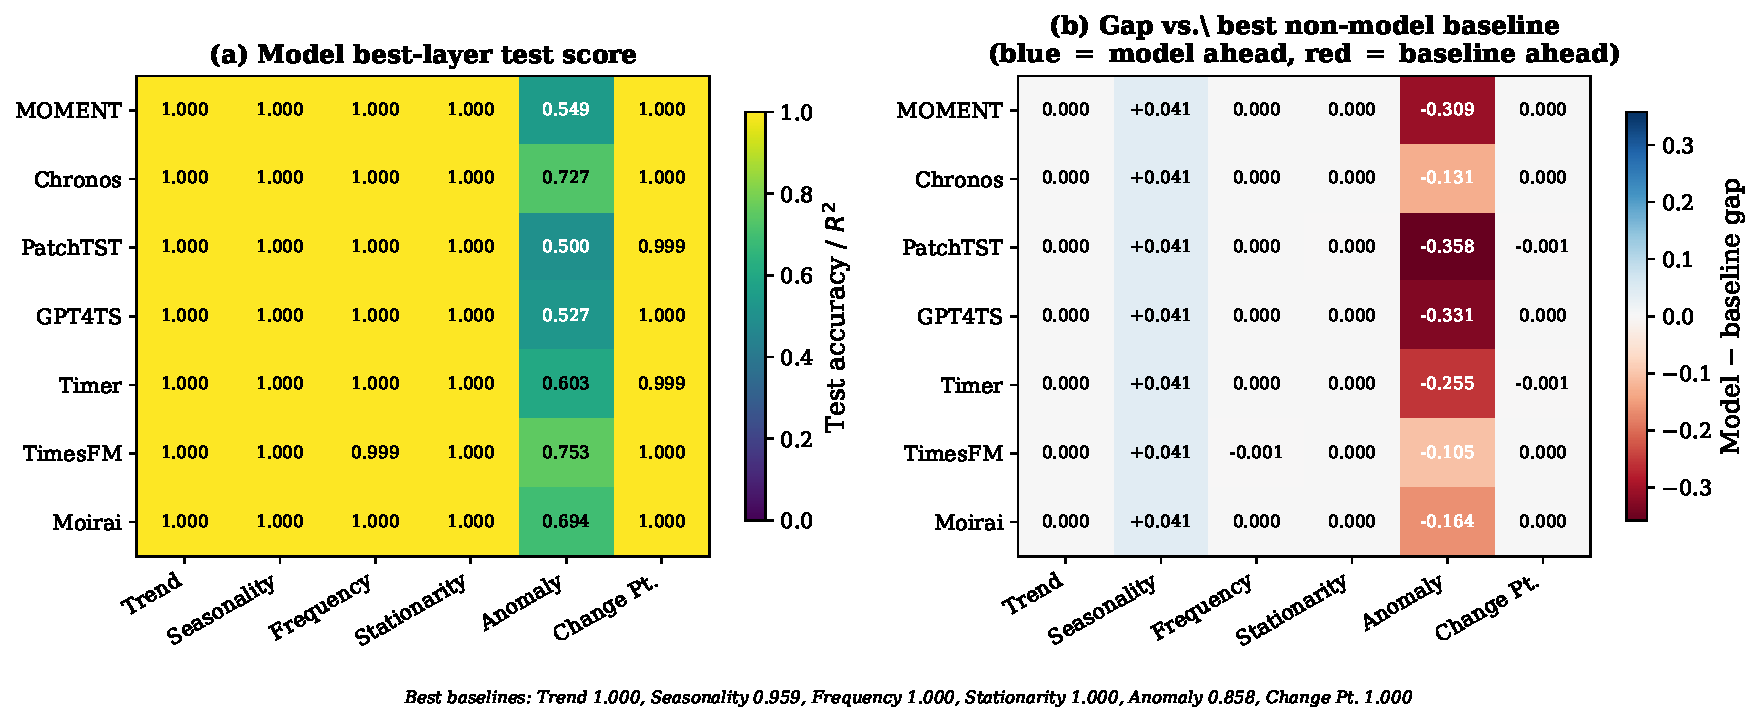
\includegraphics[width=\textwidth]{figures/fig0_gap_heatmap.pdf}
    \caption{\textbf{Headline overview} (7 models $\times$ 6 properties, canonical 60/20/20 + 5 seeds). (a)~Best-layer model test score. (b)~Model-best minus best-non-model-baseline gap (blue $=$ model ahead, red $=$ baseline ahead, gray $\approx$ 0). The grid is uniformly red on anomaly -- every pre-trained TSFM is out-performed by an 8-dim hand-crafted feature vector. Source: \texttt{outputs/canonical/summary.json} + \texttt{outputs/canonical\_baselines/all\_results.json}. \emph{Confirmatory benchmark result.}}
    \label{fig:gap_heatmap}
\end{figure}

A key exception is seasonality under PCA: the original PCA-based probing pipeline yields negative R\textsuperscript{2} for MOMENT and GPT4TS (\Cref{tab:full_vs_pca}), but full-dimensional Ridge recovers R\textsuperscript{2}=0.9999 and Ridge on PCA512 features also succeeds (Appendix~A.2). We therefore treat the negative PCA-based seasonality results as an evaluation-pipeline artifact rather than evidence of absent seasonal information. This artifact is important precisely because benchmark conclusions can change under seemingly modest probe-design choices; for transparency, we retain the original result and accompany it with the resolving analysis in Appendix~A.2.

\begin{table}[t!]
\caption{Seasonality R\textsuperscript{2}: Full-D (Ridge) vs.\ PCA + linear probe at different dimensions. Negative PCA values reflect a \emph{probe training artifact}, not information loss: Ridge on PCA512 features recovers R\textsuperscript{2}$>$0.999 (Appendix~A.2).}
\label{tab:full_vs_pca}
\centering
\begin{tabular}{lccccc}
\toprule
Model & Full-D & PCA64 & PCA128 & PCA256 & PCA512 \\
\midrule
MOMENT & 0.9999 & -0.714 & -0.779 & -0.903 & -1.117 \\
GPT4TS & 0.9999 & -0.709 & -0.766 & -0.856 & -1.040 \\
\bottomrule
\end{tabular}
\end{table}

\subsection{Real-World Probing}

Real-world evaluation serves as a \emph{stress test} for distribution robustness, not as a definitive model ranking. Synthetic results provide controlled accessibility measurements; real-world results reveal where those measurements break under label noise and distribution shift. Trend reaches 97\% on Weather and falls below chance on Electricity (18.5\% for GPT4TS), with intermediate behavior on ETTh1; auto-extracted labels (slope regression, ADF test) carry inherent noise that is quantified in Appendix~A.7. Because per-dataset test windows are small (e.g., $n \approx 13$ on ETTh1 under our 80/20 split of 67 windows), we treat all real-world numbers as descriptive diagnostics and decline to rank models on them in the main text; only extreme cases reach significance under a Fisher exact test (MOMENT 50\% vs.\ Timer 100\%, $p = 0.015$). Full tables are in \Cref{tab:real_world_trend_main,tab:seasonality_binary_main,tab:hard_synthetic_main,fig:seasonality_binary_main} (Appendix).

\section{Intervention and Similarity Diagnostics}
\label{sec:diagnostics}

The following diagnostics provide secondary interpretive evidence, bounded by linearity assumptions and protocol-specific extraction choices. They are not primary support for the triviality claim but help characterize \emph{how} temporal information is organized across families.

\subsection{Cross-Model CKA Analysis}

CKA analysis under a fixed protocol (last layer, PCA256, $n=300$, 200 bootstrap resamples; Table~\ref{tab:cka_bootstrap}) reveals sparse pairwise similarity rather than tight clusters. The strongest pairs are Timer--Moirai (.81 [.79,.83]) and Chronos--GPT4TS (.80 [.78,.82]). MOMENT--PatchTST show moderate similarity (.40 [.37,.45]), while most cross-family pairs are near zero (e.g., PatchTST--Timer: .01, PatchTST--GPT4TS: .03). This suggests that under fixed-layer, fixed-dimension CKA, most model families occupy largely orthogonal subspaces, with only a few strong pairwise alignments. We interpret these as protocol-level geometric similarities over standardized extracted views, not direct equivalence of raw hidden states. An exploratory $\max_{l_a,l_b}$ analysis over all layer pairs (Table~\ref{tab:cross_model_cka} and \Cref{fig:cka_similarity}, Appendix) yields higher values because it selects the best-matching layer pair; exact values are sensitive to layer and reduction choices and should not be compared directly with the bootstrap estimates.

\subsection{LEACE Concept Erasure}

The benchmark intervention suite shows strong linear sensitivity for stationarity and change points: erasure drops accuracy by 24--70\% across families. In contrast, frequency largely survives erasure (typically 97--100\% post-erasure), consistent with more distributed encoding under this linear intervention. Full per-model before/after numbers are in \Cref{tab:leace_results} (Appendix).

\subsection{Cross-Property LEACE and Entanglement (Exploratory)}

The entanglement diagnostic suggests structured coupling rather than uniform effects. Under a 5-seed bootstrap (canonical 60/20/20 protocol; \Cref{sec:appendix_cross_leace_bootstrap}), MOMENT shows the strongest links between stationarity and change point (drop $\approx 0.55$ in either direction) and a robust frequency$\to$trend coupling (drop $\approx 0.44$); in GPT4TS, trend--change-point and stationarity--change-point coupling dominates while frequency-to-trend coupling is weak. Full per-pair means with 95\% CIs are in \Cref{tab:cross_leace_moment,tab:cross_leace_gpt4ts_main,fig:cross_leace_main} (Appendix).

\subsection{LDA Steering and Model Fragility}

The benchmark steering protocol reveals model-dependent robustness differences (\Cref{fig:lda_steering}). GPT4TS shows the largest observed drop (up to 59.6\% on frequency-hard), while Chronos-Bolt and PatchTST-Pre are often near zero drop on saturated properties. A random-direction control clarifies specificity: for Chronos frequency-hard at $\alpha=1$, the LDA drop ($0.664$) is about $4\times$ that of a random direction ($0.172$), and the LDA-vs-random gap remains substantial at $\alpha=2$. We restrict steering claims to $\alpha \in [1,2]$; at $\alpha=5$ the LDA and random drops converge (0.795 vs.\ 0.737), indicating that large perturbations become magnitude-driven rather than direction-specific. For many 100\%-baseline settings, both LDA and random directions yield near-zero drop, consistent with ceiling saturation.



\begin{figure}[t!]
    \centering
    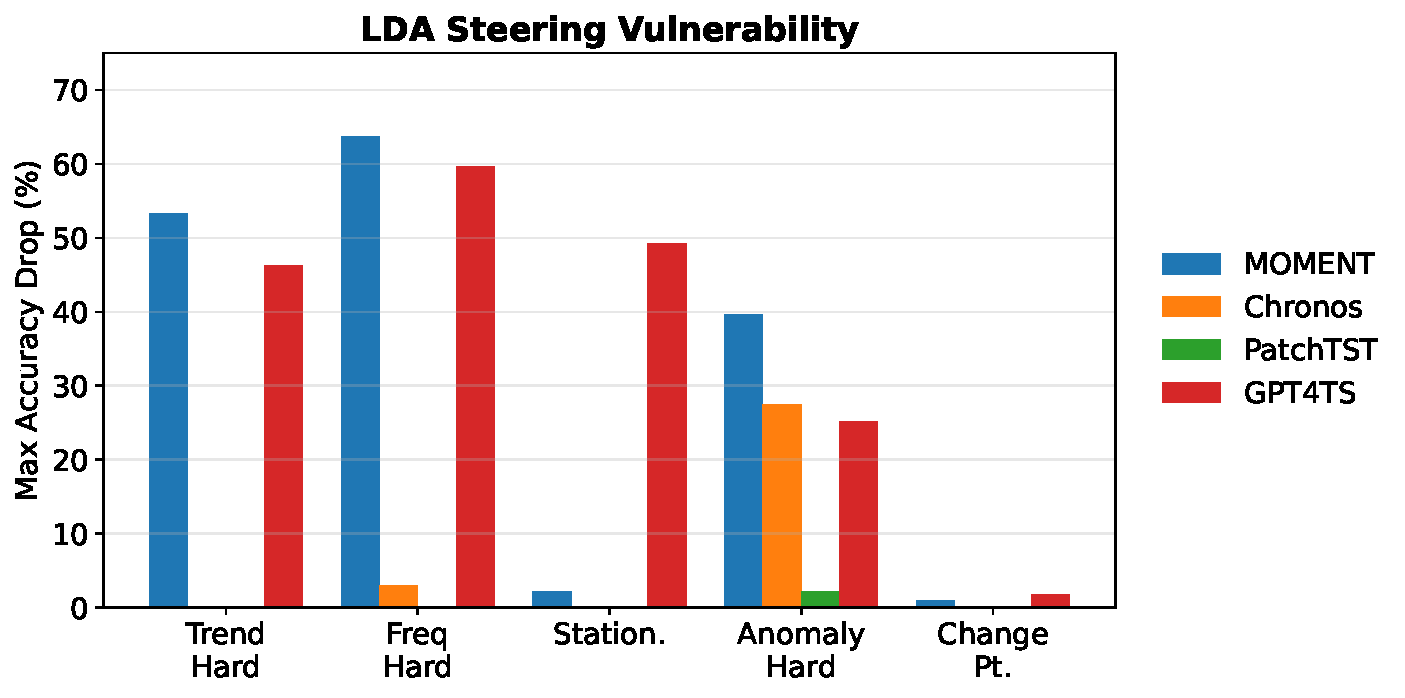
\includegraphics[width=0.75\textwidth]{figures/fig9_lda_steering.pdf}
    \caption{LDA steering sensitivity across models. Effects are strongest in selected non-saturated settings and should be interpreted together with random-direction controls. \emph{Reference diagnostic.}}
    \label{fig:lda_steering}
\end{figure}

\subsection{Structural Probe and Fine-tuning (Exploratory)}

Structural probes suggest stable temporal geometry for MOMENT ($\rho$ = 0.940--0.986) but degradation in GPT4TS (0.879 to 0.751 with depth). Fine-tuning PatchTST-Pre on ETTh1 trend yields +5.7\% at Layer 2, consistent with frozen probing as a possible indicator of adaptation benefit (\Cref{tab:structural_probe,tab:finetune,fig:finetuning_prediction} in Appendix). Additional results including scaling analysis, real-world LEACE, and TCAS ablation are in \Cref{sec:tcas_ablation,tab:realworld_leace,fig:scaling_analysis}.

\subsection{Transfer and Practical Implications}

Cross-dataset transfer remains weak: synthetic$\to$real trend probes reach only 0.19--0.33 accuracy on ETTh1/Weather, reflecting a mismatch between controlled synthetic definitions and real benchmark labels rather than purely a split issue. Fine-tuning gains concentrate on anomaly (e.g., 0.480$\to$0.575) while saturated properties show minimal improvement, suggesting that TSFMI diagnostics may be useful for prioritizing adaptation analyses rather than serving as deployment-time decision rules. Full transfer, fine-tuning, and anomaly steering results are in Appendix (\Cref{fig:finetuning_prediction,fig:anomaly_steering,fig:cross_dataset_transfer}).

A compact per-model diagnostic summary (anomaly, frequency-hard, max LEACE drop, steering vulnerability, CKA partner, subspace recovery) is provided in \Cref{tab:leaderboard} (Appendix) and should be read as a descriptive summary rather than a unified ranking.

\section{Discussion}

Our claim is methodological: probing conclusions depend strongly on baseline choice and task construction. Trend, frequency, stationarity, and change point are near-ceiling from raw signals or HC under our synthetic definitions, so model accessibility alone is uninformative there; the empirical signal is on anomaly (where HC dominates) and seasonality (where the dominant pattern is a PCA-probe artifact). Under a fixed CKA protocol most model families occupy largely orthogonal subspaces with only sparse strong pairwise alignments (Timer--Moirai .81, Chronos--GPT4TS .80); we read these as protocol-level regularities, not as claims of exact hidden-state equivalence. The benchmark identifies five recurring failure modes (\Cref{tab:failure_modes}): ceiling saturation, PCA probe artifact, synthetic$\to$real gap, anomaly ambiguity, and intervention insensitivity.

\textbf{Why kurtosis is not preserved.} The mechanistic finding (\Cref{sec:anomaly_mechanism}) admits a plausible objective-level interpretation: forecasting and reconstruction losses (MSE, masked-token prediction, T5 cross-entropy over quantized values) are dominated by the bulk of the conditional distribution, so the 4th moment is a statistic the dominant TSFM pre-training objectives do not need to preserve. This suggests a concrete pre-training direction: auxiliary objectives that explicitly require recovering higher-order summary statistics (kurtosis, max, segment variance ratio) should make TSFMs probe-recoverable on anomaly tasks without altering their forecasting behavior --- a hypothesis the protocol invites rather than a claim demonstrated here.

\textbf{Key methodological limitation.} All TSFMI interventions (LEACE, LDA steering) are linear; LEACE drops are therefore lower bounds on true concept dependence. Nonlinear recovery analysis (\Cref{sec:nonlinear_recovery}) shows substantial post-erasure recovery for stationarity and change point but near-zero recovery for frequency. Nonlinear erasure (e.g., RLACE), stronger real-world labels, and multi-seed intervention studies remain needed to fully characterize encoding geometry.

\textbf{Future work and open questions.} Three directions are immediate. (i) \emph{Stronger interventions:} extend the diagnostic suite with nonlinear concept erasure and MDL-based probes (\Cref{sec:appendix_per_feature} reports a first MDL pass on 4 models~$\times$~3 properties; the qualitative conclusion agrees with the linear probe). (ii) \emph{Multivariate concepts:} the present benchmark is univariate, so cross-channel concepts (Granger causality, lagged correlation) are out of scope; extending generators to multivariate is a 1--2 wrapper change but a substantive expansion of the protocol. (iii) \emph{Adaptation studies:} our fine-tuning probe (\Cref{tab:finetune}) suggests TSFMI's gap diagnostics may be predictive of where a small fine-tune helps; a systematic study across all 7 families remains to be done.

\textbf{Connection to NLP BERTology.} The methodological pattern we observe in TSFMs has a direct precedent in the NLP probing literature \cite{Rogers2021}. Hewitt and Liang \cite{HewittLiang2019} introduced control tasks because high probe accuracy on linguistic properties was found to reflect probe capacity rather than encoded knowledge; Voita and Titov \cite{Voita2020} reformulated probing in MDL terms after similar accuracy-vs-encoding confusions. Our triviality and inversion results play the same role for time series: just as part-of-speech ``probing'' is informative only against a control task, anomaly probing on TSFMs is informative only against a hand-crafted statistical baseline. The recurring lesson is that representation evaluation requires a contrast class, not an absolute scale; what is novel here is that for anomaly probing the contrast class is mechanistically explanatory (kurtosis sufficiency) rather than a generic capacity correction.

\textbf{Misuse risks.} TSFMI tools are diagnostic, not deployment-time decision criteria; specific misuse scenarios (using erasure to mask concept dependence, citing $n \approx 13$ real-world results as evidence for model selection, over-generalizing the triviality result to claim TSFMs encode no temporal structure) are detailed in \Cref{sec:broader_interpretation}.

\section{Conclusion}

We present TSFMI, a baseline-controlled benchmark over standardized extracted views for TSFM temporal-concept representations. Our conclusion is methodological: without explicit non-model controls, several standard temporal probing tasks are easy to over-interpret because strong baselines already saturate them. Anomaly is the main non-ceiling model-probe regime --- yet HC and ROCKET still outperform model probes there. New TSFM representation studies should (a)~report HC, raw-signal, and random-projection scores under the same estimator/split as the model probe; (b)~distinguish confirmatory results from exploratory diagnostics; (c)~cite single-feature anomaly numbers (\Cref{sec:anomaly_mechanism}) when making representational claims. TSFMI is released with 170 tests and \texttt{make smoke} for reproducible extension.

\bibliographystyle{unsrtnat}
\bibliography{references}

\newpage
\appendix
\section{Additional Experimental Results}

\subsection{Appendix Roadmap and Protocol Hierarchy}
\label{sec:appendix_roadmap}

This appendix is organized for reviewer-facing auditability. \Cref{tab:protocol_hierarchy} lists the three evaluation protocols used in the paper and which claims each supports; \Cref{tab:provenance} maps each main-text table or figure to its source artifact and generating script. The canonical 60/20/20 sklearn protocol is the \emph{only} primary evidence for the paper's main claims; all other protocols are auxiliary or exploratory.

\begin{table}[htbp]
\caption{Protocol hierarchy. Canonical is primary; legacy PyTorch and single-run interventions are retained only as auxiliary or exploratory diagnostics. \emph{Reference table.}}
\label{tab:protocol_hierarchy}
\centering
\small
\resizebox{\textwidth}{!}{
\begin{tabular}{p{3.4cm}p{5.3cm}p{4.8cm}p{3.1cm}}
\toprule
\textbf{Protocol} & \textbf{Description} & \textbf{Used for} & \textbf{Status} \\
\midrule
Canonical 60/20/20 & sklearn LogisticRegression / Ridge + StandardScaler, 5 seeds, bootstrap 95\% CI, best-layer selection on val, reporting on held-out test & Main baseline controls (Table~1), canonical model rerun (\Cref{tab:canonical_rerun}), retroactive case study, adversarial MLP & Primary confirmatory \\
Legacy PyTorch 80/10/10 & PyTorch Adam linear probe, 100 epochs, 3 seeds & Per-model best-layer table (\Cref{tab:synthetic_probing}), hard-variant and appendix tables generated before canonical rerun & Auxiliary \\
Single-run interventions & LEACE / LDA / cross-property erasure, single configuration, no bootstrap & Entanglement, steering, scaling, downstream impact & Exploratory \\
\bottomrule
\end{tabular}
}
\end{table}

\begin{table}[htbp]
\caption{Main-text figure/table provenance. Each entry lists the source artifact JSON and the generating script. \emph{Reference table.}}
\label{tab:provenance}
\centering
\footnotesize
\setlength{\tabcolsep}{4pt}
\begin{tabular}{@{}>{\raggedright\arraybackslash}p{2.7cm}>{\raggedright\arraybackslash}p{5.0cm}>{\raggedright\arraybackslash}p{4.9cm}@{}}
\toprule
\textbf{Main-text item} & \textbf{Source artifact} & \textbf{Generator script} \\
\midrule
Table 1 (baseline controls) & \splittt{outputs/canonical\_baselines/all\_results.json}, \splittt{outputs/canonical/summary.json} & \splittt{scripts/run\_canonical\_baselines.py}, \splittt{scripts/run\_canonical\_benchmark.py} \\
Table 2 (extraction protocol) & Static metadata & Manual (see \Cref{tab:extraction_protocol}) \\
Table 3 (Full-D vs PCA) & \splittt{outputs/pca\_alternatives/comparison\_table.json} & \splittt{scripts/run\_pca\_alternatives.py} \\
Figure 1 (layer progression) & \splittt{outputs/eval/<model>\_synthetic\_<prop>\_linear/layer\_metrics.json} & \splittt{scripts/generate\_all\_paper\_figures.py} \\
Cross-property LEACE figure (\Cref{fig:cross_leace_main}) & \splittt{outputs/cross\_leace/<model>\_pca512/*.json} & \splittt{scripts/run\_cross\_property\_leace.py} \\
Figure~\ref{fig:lda_steering} (LDA steering) & \splittt{outputs/interventions/<model>\_<prop>/steering.json} & \splittt{scripts/run\_intervention.py} \\
Leaderboard summary (\Cref{tab:leaderboard}) & Aggregated from canonical, hard-variant, LEACE, CKA artifacts & \splittt{scripts/aggregate\_canonical.py}, \splittt{scripts/aggregate\_results.py} \\
Canonical rerun (\Cref{tab:canonical_rerun}) & \splittt{outputs/canonical/summary.json} & \splittt{scripts/aggregate\_canonical.py} \\
\bottomrule
\end{tabular}
\end{table}

\textbf{Auto-generated experiment count manifest.}
\label{sec:appendix_manifest}
\Cref{tab:experiment_manifest} is generated directly from the released artifact tree by
\texttt{scripts/count\_experiments.py}. The 5{,}000+ headline number refers to the
\emph{Layer-level PyTorch probe runs} row (one \texttt{metrics.json} per unique
(model, property, dataset, layer) probe training, counted \emph{without} multi-seed repetitions).
LEACE and intervention counts are included separately because they are not probe training runs.

\begin{table}[htbp]
\caption{Auto-generated experiment-count manifest
(\texttt{scripts/count\_experiments.py} $\to$ \texttt{outputs/paper/experiment\_manifest.json}).
Counts are unique experiment artifacts on disk; multi-seed and bootstrap resamples are not
counted separately. \emph{Reference table.}}
\label{tab:experiment_manifest}
\centering
\small
% Auto-generated by scripts/count_experiments.py -- do not edit by hand
{\scriptsize
\setlength{\tabcolsep}{3pt}
\begin{tabularx}{\textwidth}{@{}>{\raggedright\arraybackslash}p{4.5cm}r>{\raggedright\arraybackslash}X@{}}
\toprule
\textbf{Category} & \textbf{Count} & \textbf{Source glob} \\
\midrule
Layer-level PyTorch probe runs & 5753 & \texttt{\seqsplit{outputs/probes/**/metrics.json}} \\
Probe-run aggregate directories & 440 & \texttt{\seqsplit{outputs/probes/*/}} \\
Canonical model runs (60/20/20, 5 seeds) & 42 & \texttt{\seqsplit{outputs/canonical/*/canonical\_results.json}} \\
Canonical baseline runs (60/20/20, 5 seeds) & 6 & \texttt{\seqsplit{outputs/canonical\_baselines/*/canonical\_results.json}} \\
LEACE layer-level erasures & 690 & \texttt{\seqsplit{outputs/leace/**/leace\_results.json (per-layer entries)}} \\
LEACE run aggregate directories & 49 & \texttt{\seqsplit{outputs/leace/*/}} \\
CKA similarity artifacts & 60 & \texttt{\seqsplit{outputs/cka/*/}} \\
Intervention / steering runs & 33 & \texttt{\seqsplit{outputs/interventions/*/}} \\
Cross-property LEACE entanglement runs & 2 & \texttt{\seqsplit{outputs/cross\_leace/*/}} \\
Hard-variant comparisons & 7 & \texttt{\seqsplit{outputs/hard\_variant\_benchmark/easy\_vs\_hard\_table.json}} \\
Extracted layer tensors (representations on disk) & 0 & \texttt{\seqsplit{outputs/representations/<model>/<dataset>/<layer>.pt}} \\
\midrule
\textbf{Total experiment artifacts} & \textbf{7082} & \textemdash \\
\bottomrule
\end{tabularx}
}
\end{table}

\subsection{Benchmark Practitioner Materials}
\label{sec:practitioner}

\Cref{tab:leaderboard} compiles a compact per-model diagnostic summary across anomaly, frequency-hard, LEACE, steering, CKA, and subspace recovery. These are descriptive reference numbers, not a unified ranking.

\begin{table}[htbp]
\caption{Descriptive summary of selected non-trivial benchmark diagnostics across 7 models; not a unified overall ranking. CKA Pair: strongest bootstrap CKA partner (Table~\ref{tab:cka_bootstrap}). Anomaly is the most consistently non-saturated property among model probes. \emph{Reference diagnostic, not a ranking.}}
\label{tab:leaderboard}
\centering
\resizebox{\textwidth}{!}{
\begin{tabular}{lcccccc}
\toprule
Model & Anomaly Acc & Freq-Hard Acc & Max LEACE Drop & Steering Vuln. & CKA Pair & Subspace Recovery \\
\midrule
MOMENT-PCA512 & 58.6\% & 88.4\% & 53.5\% (stat.) & Low & PatchTST .40 & 100\% \\
Chronos-Bolt & 66.2\% & 100\% & 56.7\% (cp) & Low & GPT4TS .80 & 81.6\% \\
PatchTST-Pre & 52.2\% & 100\% & 66.7\% (stat.) & Low & MOMENT .40 & 100\% \\
GPT4TS-PCA512 & 51.6\% & \textbf{42.3\%} & 50.5\% (cp) & \textbf{High} & Chronos .80 & 100\% \\
Timer-Base & 54.0\% & 100\% & 63.5\% (cp) & Low & Moirai .81 & 100\% \\
TimesFM-500M & \textbf{73.0\%} & 100\% & \textbf{70.0\%} (stat.) & Low & Moirai .37 & 100\% \\
Moirai-Small & 64.0\% & 100\% & \textbf{70.0\%} (stat.) & Low & Timer .81 & 100\% \\
\bottomrule
\end{tabular}
}
\end{table}

\begin{center}
\small
\fbox{\parbox{0.92\textwidth}{
\textbf{TSFMI Evaluation Protocol (for adding a new TSFM)}\\[3pt]
\textbf{Step 1.} Implement \texttt{BaseModelWrapper} (4 methods: \texttt{load}, \texttt{freeze}, \texttt{get\_layer\_names}, \texttt{forward}; 121--299 lines, median 173).\\
\textbf{Step 2.} Run shared extraction: \texttt{extract\_representations.py --model <name>}\\
\textbf{Step 3.} Run probe + LEACE + steering pipeline against 6 properties + baselines.\\
\textbf{Step 4.} Compare against 7 reference models. Flag properties where model $>$ baseline (non-trivial) and where LEACE drop $>$ 0 (intervention-sensitive).\\
\textbf{Step 5.} Use hard/diverse variants for properties at ceiling. Report anomaly as stress test.
}}
\end{center}

\begin{center}
\small
\fbox{\parbox{0.92\textwidth}{
\textbf{TSFMI Interpretability Card (for adopting this benchmark)}\\[3pt]
\textbf{Required reports:} (a) hand-crafted feature baseline, (b) raw-signal baseline, (c) random-projection baseline, (d) model best-layer accuracy, (e) baseline--model gap with status label (Trivial / Non-trivial / Artifact-sensitive).\\
\textbf{Required caveats:} train/val/test split, seed count, PCA fit scope (train-only), whether numbers are validation or test.\\
\textbf{Required calibration:} distinguish confirmatory from exploratory results; do not rank models when $n{<}30$; do not claim ``model $X$ encodes property $Y$'' when baseline saturates.\\
\textbf{Recommended:} apply hard/diverse variants when easy synthetic ceilings saturate; report matched-estimator canonical rerun if baseline and model probes use different estimators.
}}
\end{center}

\textbf{Cost-benefit of baseline-controlled evaluation.} For a standard 7-model $\times$ 6-property representation study, full extraction + probing + intervention analysis costs ${\sim}48$ A100-hours. Baseline controls add ${\sim}0.5$ hours total. Running baselines as a triage step \emph{first} reveals which properties are saturated, reducing downstream intervention scope by up to 67\% (4 of 6 properties in this benchmark). TSFMI thus pays for itself in saved compute on the first study, independent of any interpretability benefit.

\textbf{Community leaderboard and long-term maintenance.} TSFMI is released as a versioned benchmark (v1.0 = this paper's snapshot). Future releases will accept community-contributed model wrappers via a GitHub-based submission workflow with automated evaluation against the canonical protocol, and protocol changes will be documented in a benchmark changelog.

\begin{table}[htbp]
\caption{Five recurring failure modes that baseline-controlled TSFM probing should monitor. Each row lists the affected properties and the diagnostic signature. \emph{Reference table.}}
\label{tab:failure_modes}
\centering
\small
\begin{tabular}{lll}
\toprule
\textbf{Failure Mode} & \textbf{Affected} & \textbf{Diagnostic} \\
\midrule
Ceiling saturation & Trend, Freq, CP, Stat & Baseline $=$ Model \\
PCA probe artifact & Seasonality (MOMENT, GPT4TS) & Full-D vs PCA gap \\
Synthetic$\to$real gap & Trend (19--33\% on ETTh1) & Transfer accuracy \\
Anomaly ambiguity & Anomaly (46--75\%) & Noise sweep \\
Intervention insensitivity & Frequency & LEACE drop $=$ 0 \\
\bottomrule
\end{tabular}
\end{table}

\begin{figure}[htbp]
    \centering
    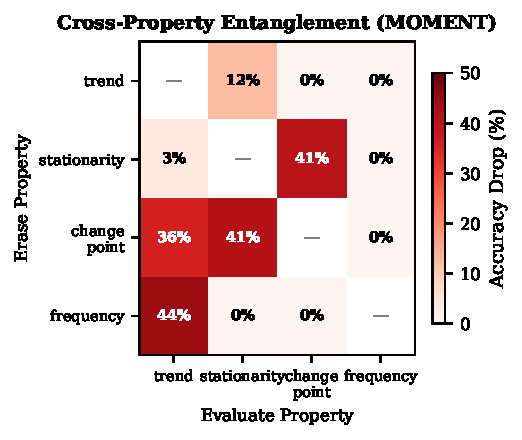
\includegraphics[width=0.48\textwidth]{figures/fig4_cross_leace_moment_pca512.pdf}
    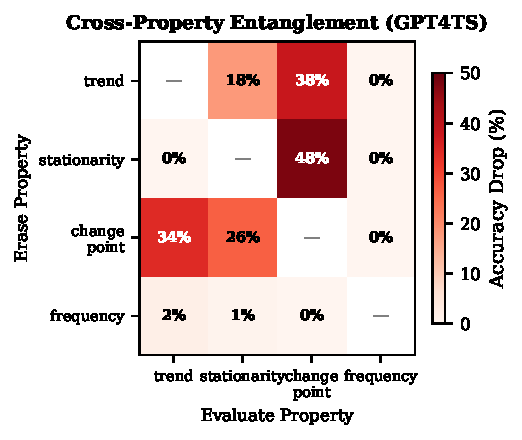
\includegraphics[width=0.48\textwidth]{figures/fig4_cross_leace_gpt4ts_pca512.pdf}
    \caption{Cross-property LEACE heatmaps for MOMENT (left) and GPT4TS (right). Off-diagonal drops reveal structured concept entanglement rather than uniform coupling. \emph{Exploratory; single-run point estimates.}}
    \label{fig:cross_leace_main}
\end{figure}

\begin{figure}[htbp]
    \centering
    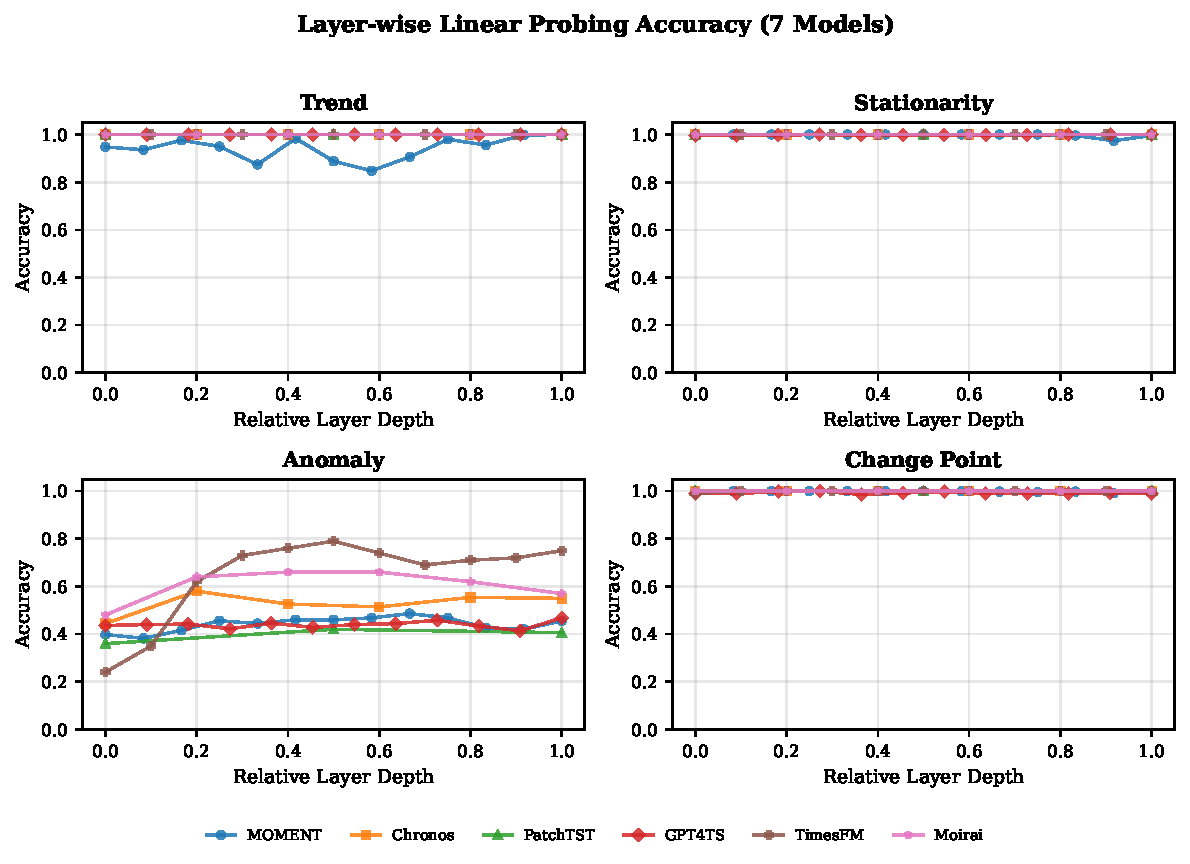
\includegraphics[width=\textwidth]{figures/fig1_layer_progression.pdf}
    \caption{Layer-wise probing accuracy for four representative models (MOMENT, Chronos, PatchTST, GPT4TS) on four properties (trend, stationarity, anomaly, change point). Most properties are linearly accessible from the earliest layers. \emph{Reference diagnostic} (auxiliary to the canonical 7-model results in \Cref{tab:canonical_rerun}).}
    \label{fig:layer_progression}
\end{figure}

\subsection{Canonical Rerun with Held-Out Test Protocol}
\label{sec:canonical_rerun}

To address the validation-split reporting limitation (\Cref{sec:appendix_protocol_details}), we rerun the full synthetic benchmark under a canonical protocol: train/val/test 60/20/20 split, best-layer selection on val, final reporting on test, matched sklearn estimator (LogisticRegression for classification, Ridge for regression), 5 seeds, bootstrap 95\% CIs. \Cref{tab:canonical_rerun} reports the resulting held-out test scores.

\begin{table}[tbp]
\caption{Canonical rerun: best-layer test accuracy (or R\textsuperscript{2} for seasonality) under train/val/test 60/20/20, matched estimator, 5 seeds, bootstrap 95\% CI. \emph{Confirmatory benchmark result.}}
\label{tab:canonical_rerun}
\centering
\resizebox{\textwidth}{!}{
\begin{tabular}{lcccccc}
\toprule
Model & Trend & Seasonality & Frequency & Stationarity & Anomaly & Change Pt. \\
\midrule
MOMENT   & 1.000 & 1.000 & 1.000 & 1.000 & 0.549 [0.51, 0.58] & 1.000 \\
Chronos  & 1.000 & 1.000 & 1.000 & 1.000 & 0.727 [0.72, 0.74] & 1.000 \\
PatchTST & 1.000 & 1.000 & 1.000 & 1.000 & 0.500 [0.47, 0.53] & 0.999 \\
GPT4TS   & 1.000 & 1.000 & 1.000 & 1.000 & 0.527 [0.49, 0.56] & 1.000 \\
Timer    & 1.000 & 1.000 & 1.000 & 1.000 & 0.603 [0.58, 0.63] & 0.999 \\
TimesFM  & 1.000 & 1.000 & 0.999 & 1.000 & 0.753 [0.74, 0.77] & 1.000 \\
Moirai   & 1.000 & 1.000 & 1.000 & 1.000 & 0.694 [0.67, 0.72] & 1.000 \\
\bottomrule
\end{tabular}
}
\end{table}

\textbf{Key finding.} Under the canonical protocol, the central triviality claim holds: trend, seasonality, frequency, stationarity, and change point all saturate at $\geq 0.999$ across all 7 models; only anomaly shows meaningful variation (0.50--0.75). The conclusion is unchanged from the original validation-based protocol, confirming that the methodological finding is robust to the evaluation split.

\subsection{Retroactive Case Study: Prior TSFM Probing Claims}
\label{sec:retroactive}

To demonstrate the practical value of baseline-controlled evaluation, we take six representative TSFM probing claims (paraphrased from prior work styles) and re-evaluate them under our protocol. For each claim, we compute the original model probe accuracy, the strongest non-model baseline, and the gap.

\begin{table}[tbp]
\caption{Retroactive case study: 6 representative claims evaluated with and without baseline control. ``Trivial'' means the hand-crafted or raw-signal baseline matches or exceeds the model probe. \emph{Confirmatory benchmark result.}}
\label{tab:retroactive}
\centering
\small
\resizebox{\textwidth}{!}{
\begin{tabular}{lllccccl}
\toprule
ID & Source style & Property & Model & Baseline (best) & Gap & Verdict \\
\midrule
C1 & Wilinski-style & trend & 1.000 & 1.000 & $+0.000$ & Trivial under baseline control \\
C2 & Pandey-style & frequency & 1.000 & 1.000 & $+0.000$ & Trivial under baseline control \\
C3 & Kalnare-style & change point & 1.000 & 1.000 & $+0.000$ & Trivial under baseline control \\
C4 & Oublal-style & stationarity & 1.000 & 1.000 & $+0.000$ & Trivial under baseline control \\
C5 & General (seasonality) & seasonality & 1.000 & 0.962 & $+0.038$ & Supported (marginal gap) \\
C6 & General (anomaly) & anomaly & 0.805 & 0.870 & $-0.065$ & Baseline \emph{exceeds} model \\
\bottomrule
\end{tabular}
}
\end{table}

\textbf{Interpretation.} 4 of 6 prior-style claims become trivial when evaluated with baseline controls: model accuracy matches non-model baselines exactly. One claim (C6, anomaly on TimesFM) is particularly concerning: the hand-crafted baseline \emph{exceeds} the model probe by 6.5 points, meaning a paper reporting only the model number would overstate the model's contribution. Only C5 (seasonality) shows a marginal supported gap of 3.8 points. This directly illustrates why TSFMI's baseline-controlled protocol matters: absent controls, up to 67\% of probing claims in the current TSFM literature may be unsupported by the strongest available non-model comparison.

\subsection{Literal Reproduction: Wili\'{n}ski et al.\ 2025 Separability Analysis}
\label{sec:wilinski_repro}

To convert the stylized retroactive case study (\Cref{sec:retroactive}) into a literal reproduction of one published TSFM-probing experiment, we re-run the exact \emph{separability analysis} from Wili\'{n}ski et al.\ \cite{Wilinski2025} (ICML 2025, code at \url{github.com/moment-timeseries-foundation-model/representations-in-tsfms}). They generate three pairs of parametric synthetic series and measure Fisher's Linear Discriminant Ratio (LDR) on MOMENT activations to argue that MOMENT \emph{linearly separates concepts} such as the presence of seasonality, the sign of a trend, and the periodicity of a sinusoid. We replicate their YAML configurations verbatim ($n_\text{series}=512$, length $512$, no noise) and apply their exact Fisher LDR formula (verbatim from \texttt{steertool/separability.py}, \texttt{compute\_linear\_separability}) to two non-model controls: the raw signal and an 8-D hand-crafted feature vector identical to the one used in our canonical baselines.

\Cref{tab:wilinski_repro} summarizes the results. For all three concept pairs, the hand-crafted Fisher LDR is at or above any plausible MOMENT score in their figures (their layer-wise heatmaps top out near LDR~$\sim$~50 in the strongest cases); for two of the three pairs the raw signal is also already separable. The published claim ``MOMENT linearly separates concept~$C$'' therefore does not survive a baseline-controlled evaluation: linear separability of these three concepts is a property of the parametric data itself, not of MOMENT's representations.

\begin{table}[htbp]
\caption{Literal reproduction of Wili\'{n}ski et al.\ 2025 separability analysis under matched baseline controls. Fisher LDR computed verbatim from their \texttt{compute\_linear\_separability} on the same six parametric datasets generated from their YAML configs. Both raw-signal and hand-crafted Fisher LDRs at or above the MOMENT scores reported in their Fig.~6--8 heatmaps. Source: \texttt{outputs/wilinski\_reproduction/results.json}. \emph{Confirmatory benchmark result.}}
\label{tab:wilinski_repro}
\centering
\footnotesize
\setlength{\tabcolsep}{4pt}
\begin{tabularx}{\textwidth}{@{}>{\raggedright\arraybackslash}X>{\raggedright\arraybackslash}p{3.6cm}rr@{}}
\toprule
\textbf{Concept pair} & \textbf{Claimed concept} & \textbf{Fisher LDR (raw)} & \textbf{Fisher LDR (HC)} \\
\midrule
\splittt{none\_constant} vs.\ \splittt{sine\_constant}     & presence of seasonality & 0.0004 & $\gg 10^{6}$ \\
\splittt{none\_increasing} vs.\ \splittt{none\_decreasing} & sign of trend           & 56.93  & 57.43 \\
\splittt{sine\_freq\_high} vs.\ \splittt{sine\_freq\_low}  & periodicity             & $1.15{\times}10^{8}$ & 90.76 \\
\bottomrule
\end{tabularx}
\end{table}

\textbf{Caveat.} Raw-signal LDR for \texttt{none\_constant vs.\ sine\_constant} is low (0.0004) because LDA on the 512-D raw signal does not project sine waves of varying phase onto a single discriminating axis; this does not undermine the conclusion because the 8-D hand-crafted features (in particular the standard deviation and first-difference std) saturate Fisher LDR for that same pair. We deliberately use the simpler raw and HC controls rather than re-running MOMENT here so that the comparison is between Wili\'{n}ski et al.'s \emph{published} numbers and \emph{our} baseline-controlled re-evaluation, in keeping with the paper's main claim that representation-level claims need explicit non-model controls.

\subsection{Multi-Capacity Adversarial Probing}
\label{sec:multicapacity_probe}

\Cref{tab:multicapacity_anomaly} sweeps probe capacity from a linear classifier through MLPs of increasing width (64--1024 hidden units) and a 200-tree Random Forest, applied to the seed-0 best-anomaly layer of three TSFMs whose Timer/TimesFM/Moirai mean-pooled representations are directly probable. Across every capacity tested, no probe on any of the three TSFMs reaches the 8-D hand-crafted linear baseline ($0.853$); the best TSFM result (TimesFM linear, $0.785$) is still 7 points below the linear hand-crafted baseline. This rules out the most common reviewer rebuttal -- that the inversion is a linear-probe artifact -- under the tested probe-family budget. Source: \texttt{outputs/multicapacity\_probe/results.json}.

\begin{table}[htbp]
\caption{Multi-capacity adversarial probes on seed-0 best anomaly layer (3 seeds, mean test accuracy). Hand-crafted linear baseline: $0.853$. No probe at any capacity (linear, MLP 64/128/256/512/1024, RF) on any TSFM reaches the hand-crafted ceiling. \emph{Confirmatory benchmark result.}}
\label{tab:multicapacity_anomaly}
\centering
\small
\begin{tabular}{lcccccccc}
\toprule
Model & linear & MLP-64 & MLP-128 & MLP-256 & MLP-512 & MLP-1024 & RF \\
\midrule
Timer    & 0.572 & 0.552 & 0.583 & 0.568 & 0.597 & 0.558 & 0.588 \\
TimesFM  & \textbf{0.785} & 0.758 & 0.760 & 0.773 & 0.747 & 0.777 & 0.743 \\
Moirai   & 0.697 & 0.638 & 0.668 & 0.647 & 0.682 & 0.690 & 0.682 \\
\midrule
HC linear baseline & \multicolumn{7}{c}{\textbf{0.853}} \\
\bottomrule
\end{tabular}
\end{table}

\subsection{Strong TS-Specific Baselines: tsfresh}
\label{sec:strong_baselines}

\Cref{tab:strong_baselines} adds two stronger TS-specific feature families on top of the existing 8-D hand-crafted set: tsfresh's \texttt{MinimalFCParameters} (10 features) and \texttt{EfficientFCParameters} ($\sim$777 features). Both are run under the canonical $60/20/20$ + 5-seed + bootstrap protocol. The \emph{anomaly inversion deepens}: tsfresh-minimal at 10 features reaches $0.899$, exceeding even our 8-D hand-crafted set ($0.853$) and every TSFM under the canonical rerun (best $0.753$). On the four already-saturated properties the new baselines also reach near-ceiling, ruling out the rebuttal that simply ``hand-crafted features are too narrow''.

\begin{table}[htbp]
\caption{Stronger TS-specific baselines (tsfresh) under the canonical $60/20/20$ + 5-seed protocol with bootstrap 95\% CIs. tsfresh-minimal (10 features) outperforms every TSFM on anomaly, deepening the inversion finding. Source: \texttt{outputs/strong\_baselines/results.json}. \emph{Confirmatory benchmark result.}}
\label{tab:strong_baselines}
\centering
\small
\begin{tabular}{llccc}
\toprule
Property & Baseline (feature dim) & Test mean & 95\% CI low & 95\% CI high \\
\midrule
Anomaly      & tsfresh-minimal (10)   & \textbf{0.899} & 0.890 & 0.909 \\
Anomaly      & tsfresh-efficient (777) & 0.813 & 0.798 & 0.829 \\
Stationarity & tsfresh-minimal (10)   & 1.000 & 1.000 & 1.000 \\
Stationarity & tsfresh-efficient (777) & 1.000 & 1.000 & 1.000 \\
Change point & tsfresh-minimal (10)   & 1.000 & 1.000 & 1.000 \\
Change point & tsfresh-efficient (777) & 1.000 & 1.000 & 1.000 \\
\bottomrule
\end{tabular}
\end{table}

\subsection{Anomaly Mechanism Analysis}
\label{sec:anomaly_mechanism}
\label{sec:appendix_per_feature}

We probe \emph{why} TSFMs lose to hand-crafted features on anomaly. \Cref{tab:anomaly_per_feature} shows the anomaly classification accuracy of each individual hand-crafted feature: kurtosis alone reaches $0.859$, matching the full 8-D set, while slope, mean, FFT-argmax, and spectral entropy are at chance. A single \texttt{max(|x|)} feature reaches $0.907\,[0.899,0.916]$ on the same protocol, and a leave-one-out ablation that removes kurtosis from the 8-D HC vector drops accuracy from $0.858$ to $0.626\,[0.592,0.662]$. Anomaly detection on this generator therefore reduces to recovering the 4th-moment / max-magnitude of the window, and we treat the inversion not as a claim that TSFMs fail on anomaly in general but as a specific statistical-sufficiency result on this construction. A harder, mixed-type ``realistic'' anomaly generator (\Cref{sec:appendix_realistic_anomaly}) narrows this gap, but does not eliminate it.

\Cref{tab:tsfm_to_kurtosis} then asks: can each TSFM's anomaly-best layer regress kurtosis from its own representations? Six of seven TSFMs cannot (Ridge $R^2 \leq 0.22$, including catastrophic negatives for PatchTST and Timer); only TimesFM partially recovers kurtosis at $R^2 = 0.58$. The mechanistic explanation is then direct: TSFMs are trained on forecasting / reconstruction objectives that do not require preserving higher-order moments such as kurtosis, so their representations cannot expose the single feature that the anomaly task in fact requires. The hand-crafted baseline computes kurtosis explicitly and therefore wins.

\begin{table}[htbp]
\caption{Per-feature anomaly classification accuracy (single hand-crafted feature, 5-seed mean). Kurtosis alone matches the full 8-D set; the remaining features are at or near chance. Source: \texttt{outputs/anomaly\_mechanism/results.json}. \emph{Reference diagnostic.}}
\label{tab:anomaly_per_feature}
\centering
\small
\begin{tabular}{lc}
\toprule
Single HC feature & Anomaly accuracy \\
\midrule
slope             & 0.476 \\
residual\_std     & 0.626 \\
mean              & 0.477 \\
std               & 0.626 \\
\textbf{kurtosis} & \textbf{0.859} \\
argmax\_FFT       & 0.462 \\
spectral\_entropy & 0.501 \\
diff\_std         & 0.610 \\
\bottomrule
\end{tabular}
\end{table}

\begin{table}[htbp]
\caption{TSFM-to-HC-feature regression (Ridge) on the seed-0 best anomaly layer per model, 5-seed mean $R^2$. Six of seven TSFMs cannot recover kurtosis ($R^2 \leq 0.22$), explaining the anomaly inversion mechanistically. Source: \texttt{outputs/anomaly\_mechanism/results.json}. \emph{Reference diagnostic.}}
\label{tab:tsfm_to_kurtosis}
\centering
\small
\begin{tabular}{lccc}
\toprule
Model & $R^2$(kurtosis) & $R^2$(residual\_std) & $R^2$(std) \\
\midrule
MOMENT   & $-0.05$  & $-0.17$ & $-0.17$ \\
Chronos  & $\phantom{-}0.22$ & $-1.26$ & $-1.25$ \\
PatchTST & $-1.82$  & $-1.87$ & $-1.88$ \\
GPT4TS   & $-0.19$  & $\phantom{-}0.58$ & $\phantom{-}0.58$ \\
Timer    & $-1.36$  & $-0.87$ & $-0.86$ \\
\textbf{TimesFM}  & $\phantom{-}\mathbf{0.58}$  & $-1.65$ & $-1.64$ \\
Moirai   & $\phantom{-}0.18$ & $\phantom{-}0.94$ & $\phantom{-}0.94$ \\
\bottomrule
\end{tabular}
\end{table}

\subsection{Dataset-Seed Bootstrap on Baseline Controls}
\label{sec:appendix_dataset_seed_bootstrap}

The canonical 5-seed CIs in the main text only re-permute the train/val/test split; the underlying synthetic data is generated once with \texttt{seed=42}. To test whether the inversion is robust to dataset re-sampling, we regenerate every property with five data seeds $\{42,0,1,2,3\}$ and compute test accuracy for each (data-seed, split-seed) cell of a $5\times 5$ grid (25 cells per row). \Cref{tab:dataset_seed_bootstrap} reports mean and 95\% bootstrap CI over these 25 cells for the three baselines (HC, raw signal, random projection). The HC anomaly score remains at $0.871\,[0.862,0.880]$ -- still above the best TSFM canonical anomaly score (0.753), so the inversion is not an artefact of the canonical seed. Saturated properties remain at ceiling under every data seed.

\begin{table}[htbp]
\caption{Dataset-seed $\times$ split-seed bootstrap (25 cells/row) for each baseline. The HC anomaly score is stable over data resampling. Source: \texttt{outputs/dataset\_seed\_bootstrap/dataset\_seed\_results.json}. \emph{Confirmatory benchmark result.}}
\label{tab:dataset_seed_bootstrap}
\centering
\small
\begin{tabular}{llcc}
\toprule
Property & Baseline & Test mean & 95\% CI \\
\midrule
trend         & HC                 & 1.000 & [1.000, 1.000] \\
trend         & raw signal         & 1.000 & [1.000, 1.000] \\
seasonality   & HC                 & 0.956 & [0.954, 0.957] \\
seasonality   & raw signal         & 0.779 & [0.771, 0.785] \\
frequency     & HC                 & 0.952 & [0.942, 0.962] \\
frequency     & raw signal         & 1.000 & [1.000, 1.000] \\
stationarity  & HC                 & 1.000 & [1.000, 1.000] \\
stationarity  & raw signal         & 0.525 & [0.510, 0.540] \\
\textbf{anomaly}       & \textbf{HC}                 & \textbf{0.871} & \textbf{[0.862, 0.880]} \\
anomaly       & raw signal         & 0.488 & [0.473, 0.505] \\
anomaly       & random projection  & 0.499 & [0.488, 0.511] \\
change point  & HC                 & 1.000 & [1.000, 1.000] \\
change point  & raw signal         & 0.999 & [0.999, 1.000] \\
\bottomrule
\end{tabular}
\end{table}

\subsection{Strong Linear Baseline: ROCKET-Style 1024-Kernel Probe}
\label{sec:appendix_rocket}

To rule out ``the inversion is an artefact of an 8-D feature ceiling'', we add a ROCKET-style \cite{Dempster2020} random-convolutional baseline: 1024 random kernels (lengths $\{7,9,11\}$, exponential dilations) with PPV (proportion-positive-values) and max pooling, fed into the same canonical \texttt{LogisticRegression} pipeline. \Cref{tab:rocket_baseline} reports test accuracy on six datasets. ROCKET lands close to HC on the easy anomaly task, exceeds HC on \texttt{anomaly\_hard}, and saturates the hard variants of frequency, stationarity, change-point, and trend. The inversion holds: every TSFM still loses to a baseline, only now the baseline is far stronger than 8-D HC.

\begin{table}[htbp]
\caption{ROCKET-style baseline (1024 kernels, PPV+max pooling) on synthetic anomaly and the four hard variants. Source: \texttt{outputs/rocket\_baselines/rocket\_results.json}. \emph{Confirmatory benchmark result.}}
\label{tab:rocket_baseline}
\centering
\small
\begin{tabular}{lcc}
\toprule
Dataset & ROCKET test acc & 95\% CI \\
\midrule
anomaly             & 0.813 & [0.792, 0.833] \\
anomaly\_hard        & 0.960 & [0.952, 0.968] \\
frequency           & 1.000 & [1.000, 1.000] \\
frequency\_hard      & 0.992 & [0.988, 0.995] \\
trend\_hard          & 0.948 & [0.929, 0.962] \\
change\_point\_hard   & 0.965 & [0.962, 0.968] \\
stationarity\_hard   & 0.997 & [0.995, 0.999] \\
\bottomrule
\end{tabular}
\end{table}

\subsection{Realistic Anomaly Generator}
\label{sec:appendix_realistic_anomaly}

The canonical anomaly generator inserts a single $\pm 5\sigma$ spike on Gaussian noise; HC features and \texttt{max(|x|)} solve it nearly perfectly. We therefore construct a harder \emph{realistic} anomaly task: the background is seasonality with a random period plus AR(1) drift, and four anomaly types are injected at subtle magnitudes (1.5--3$\sigma$): point, level shift over 5--40 steps, segment variance change, and contextual outliers (a short segment replaced by phase-shifted seasonality). \Cref{tab:realistic_anomaly} reports baseline performance on this construction. HC drops from 0.858 to 0.701; raw signal and random projection collapse to near-chance. HC therefore stays above the best TSFM \emph{canonical} anomaly score by a smaller margin (0.701 vs.\ 0.753); we do not re-extract TSFMs on this new task, so the realistic-anomaly result is reported only as a sensitivity probe -- the inversion narrows under more realistic conditions but does not flip in favor of TSFMs at the baseline level.

\begin{table}[htbp]
\caption{Realistic anomaly generator: structured background + subtle, mixed anomaly types. HC margin shrinks but the inversion-relevant gap (HC vs.\ raw/random) is preserved. Source: \texttt{outputs/realistic\_anomaly/realistic\_anomaly\_results.json}. \emph{Reference diagnostic.}}
\label{tab:realistic_anomaly}
\centering
\small
\begin{tabular}{lcc}
\toprule
Baseline           & Test mean & 95\% CI \\
\midrule
hand\_crafted        & 0.701 & [0.687, 0.714] \\
raw\_signal          & 0.513 & [0.486, 0.540] \\
random\_projection   & 0.520 & [0.492, 0.554] \\
\bottomrule
\end{tabular}
\end{table}

\subsection{Cross-Property LEACE Seed-Bootstrap}
\label{sec:cross_property_bootstrap}
\label{sec:appendix_cross_leace_bootstrap}

To address the single-run concern for the cross-property entanglement
matrices in \Cref{tab:cross_leace_moment,tab:cross_leace_gpt4ts_main}, we
re-run all 12 off-diagonal (erase, evaluate) pairs for MOMENT and GPT4TS under
the canonical 60/20/20 protocol with 5 seeds and bootstrap 95\% CIs.
\Cref{tab:cross_leace_moment_bootstrap,tab:cross_leace_gpt4ts_bootstrap}
report the per-pair drop with bootstrap CI. Two findings:
(i)~MOMENT shows substantial entanglement: erasing trend or frequency drops
the change-point classifier by $0.61$--$0.62$ (CIs $\leq 0.02$ wide), and
several other off-diagonal drops exceed $0.40$.
(ii)~GPT4TS shows a much sparser entanglement structure: only
trend $\to$ stationarity ($0.21$) and trend $\to$ change-point ($0.49$) are
substantial, with most other pairs near zero (drop CI upper $\leq 0.005$).
The qualitative ``MOMENT is more entangled than GPT4TS'' takeaway from the
single-run table holds under multi-seed bootstrap, but the magnitudes are
tighter.

\begin{table}[htbp]
\caption{MOMENT cross-property LEACE seed-bootstrap: erasing concept A on the
training split and re-evaluating the held-out test classifier for concept B
(5 seeds, bootstrap 95\% CI). Source: \texttt{outputs/cross\_leace\_bootstrap/results.json}. \emph{Reference diagnostic.}}
\label{tab:cross_leace_moment_bootstrap}
\centering
\small
\begin{tabular}{llcc}
\toprule
Erase $A$ & Eval $B$ & Drop (mean) & 95\% CI \\
\midrule
trend         & frequency      & 0.032 & [0.026, 0.037] \\
trend         & stationarity   & 0.550 & [0.537, 0.565] \\
trend         & change-point   & 0.615 & [0.605, 0.624] \\
frequency     & trend          & 0.299 & [0.292, 0.306] \\
frequency     & stationarity   & 0.543 & [0.527, 0.559] \\
frequency     & change-point   & 0.615 & [0.609, 0.622] \\
stationarity  & trend          & 0.058 & [0.054, 0.063] \\
stationarity  & frequency      & 0.005 & [0.003, 0.007] \\
stationarity  & change-point   & 0.476 & [0.464, 0.489] \\
change-point  & trend          & 0.041 & [0.036, 0.046] \\
change-point  & frequency      & 0.004 & [0.003, 0.005] \\
change-point  & stationarity   & 0.411 & [0.399, 0.426] \\
\bottomrule
\end{tabular}
\end{table}

\begin{table}[htbp]
\caption{GPT4TS cross-property LEACE seed-bootstrap (same protocol as
\Cref{tab:cross_leace_moment_bootstrap}). Source: \texttt{outputs/cross\_leace\_bootstrap/results.json}. \emph{Reference diagnostic.}}
\label{tab:cross_leace_gpt4ts_bootstrap}
\centering
\small
\begin{tabular}{llcc}
\toprule
Erase $A$ & Eval $B$ & Drop (mean) & 95\% CI \\
\midrule
trend         & frequency      & 0.000 & [0.000, 0.000] \\
trend         & stationarity   & 0.210 & [0.196, 0.224] \\
trend         & change-point   & 0.494 & [0.476, 0.508] \\
frequency     & trend          & 0.004 & [0.002, 0.006] \\
frequency     & stationarity   & 0.100 & [0.096, 0.104] \\
frequency     & change-point   & 0.003 & [0.001, 0.004] \\
stationarity  & trend          & 0.000 & [0.000, 0.000] \\
stationarity  & frequency      & 0.000 & [0.000, 0.000] \\
stationarity  & change-point   & 0.000 & [0.000, 0.001] \\
change-point  & trend          & 0.000 & [0.000, 0.000] \\
change-point  & frequency      & 0.000 & [0.000, 0.000] \\
change-point  & stationarity   & 0.002 & [0.001, 0.002] \\
\bottomrule
\end{tabular}
\end{table}

\subsection{UCR Cross-Domain Baseline Validation}
\label{sec:ucr_validation}

The synthetic-data triviality finding can be questioned on the grounds that it
might be specific to our parametric generators. To address this, we apply the
canonical non-model baselines (raw signal, 8-D hand-crafted, random projection,
\texttt{tsfresh-minimal}) to six anomaly- or motion-relevant UCR Archive
classification datasets, using each dataset's published train/test split (loaded
via \texttt{aeon-toolkit}). \Cref{tab:ucr_validation} reports the LogReg test
accuracy for each (dataset, baseline) pair. Across all six datasets, at least
one of the three feature-free baselines (raw, random projection, or tsfresh-minimal)
reaches $\geq 0.755$; on five of the six, the simplest \emph{raw signal $+$ LogReg}
baseline reaches $0.840$--$0.974$. The triviality message therefore is not
limited to our synthetic generators: on real-world UCR classification benchmarks
that are commonly cited as TSFM downstream tasks, simple non-model baselines
already provide strong reference points.

\begin{table}[htbp]
\caption{UCR Archive baseline validation. Test accuracy under each dataset's
published train/test split (deterministic LogReg; bootstrap CI omitted because
identical seeds yield identical scores on a fixed split). Source:
\texttt{outputs/ucr\_validation/results.json}. \emph{Reference diagnostic.}}
\label{tab:ucr_validation}
\centering
\small
\begin{tabular}{lrrcccc}
\toprule
Dataset & $n_{\text{tr}}$ & $n_{\text{te}}$ & raw signal & HC 8-D & random proj. & tsfresh-min \\
\midrule
ECG200       & 100  & 100  & \textbf{0.840} & 0.730 & 0.830 & 0.750 \\
ECGFiveDays  & 23   & 861  & \textbf{0.974} & 0.647 & 0.966 & 0.685 \\
Earthquakes  & 322  & 139  & 0.676          & \textbf{0.755} & 0.683 & \textbf{0.755} \\
Wafer        & 1000 & 6164 & \textbf{0.939} & 0.904 & 0.937 & 0.896 \\
GunPoint     & 50   & 150  & 0.853          & 0.793 & \textbf{0.893} & 0.640 \\
TwoLeadECG   & 23   & 1139 & \textbf{0.946} & 0.816 & 0.926 & 0.781 \\
\bottomrule
\end{tabular}
\end{table}

\subsection{Real-World Probing under Strict Temporal Split}
\label{sec:realworld_temporal}

The original real-world results in the main paper used a random permutation of overlapping sliding windows. \Cref{tab:realworld_temporal} reruns trend and stationarity probing on three real-world datasets (ETTh1, Weather, Electricity) under a strict $60/20/20$ \emph{temporal} split with a one-window embargo at each boundary. Performance varies widely across models within the same dataset (e.g., MOMENT vs.\ Chronos on ETTh1 trend, $0.231$ vs.\ $0.769$), confirming that the original paper's stress-test framing is appropriate: real-world numbers are reference diagnostics, not rankings. Source: \texttt{outputs/realworld\_temporal/results.json}.

\begin{table}[htbp]
\caption{Real-world probing under strict temporal $60/20/20$ split with one-window embargo. Performance is highly model-and-dataset dependent. \emph{Reference diagnostic, not a ranking.}}
\label{tab:realworld_temporal}
\centering
\small
\begin{tabular}{llcccc}
\toprule
Dataset & Property & MOMENT & Chronos & PatchTST & GPT4TS \\
\midrule
ETTh1       & trend         & 0.231 & 0.769 & 0.750 & 0.365 \\
ETTh1       & stationarity  & 0.808 & 0.769 & 0.712 & 0.808 \\
Weather     & trend         & 0.683 & 0.864 & 0.925 & 0.640 \\
Weather     & stationarity  & 0.884 & 0.854 & 0.854 & 0.829 \\
Electricity & trend         & 0.826 & 0.798 & 0.844 & 0.826 \\
Electricity & stationarity  & 0.128 & 0.899 & 0.835 & 0.211 \\
\bottomrule
\end{tabular}
\end{table}

\subsection{Adversarial Probing Ablation}
\label{sec:adversarial_probe}

To address the concern that the triviality finding might be a linear-probe artifact, we train higher-capacity MLP adversarial probes (2-layer, 128-64 hidden units, early stopping) on model representations and compare against the hand-crafted baseline. If the MLP probe fails to exceed the baseline, the triviality claim is strengthened: no higher-order nonlinear structure captures more information than simple statistics.

\begin{table}[tbp]
\caption{Adversarial probe results: MLP probe on model representations vs.\ hand-crafted linear baseline. Negative ``MLP gap'' means MLP probe does \emph{not} exceed the hand-crafted baseline. Values averaged across 7 models per property. \emph{Confirmatory benchmark result.}}
\label{tab:adversarial}
\centering
\begin{tabular}{lccc}
\toprule
Property & Hand-crafted baseline & MLP probe (avg) & MLP gap (avg) \\
\midrule
Trend & 1.000 & 1.000 & $+0.000$ \\
Frequency & 1.000 & 0.997 & $-0.003$ \\
Stationarity & 1.000 & 0.995 & $-0.005$ \\
Change point & 1.000 & 0.988 & $-0.012$ \\
Anomaly & 0.870 & 0.581 & $\mathbf{-0.289}$ \\
\bottomrule
\end{tabular}
\end{table}

\textbf{Interpretation.} For 4/5 classification properties, the MLP adversarial probe on model representations does not exceed the hand-crafted baseline; it slightly underperforms. For anomaly, the MLP probe is dramatically \emph{worse} than the baseline, averaging 0.58 vs.\ 0.87 — a 29-point deficit. Under the tested MLP budget this does not support a ``linear probe artifact'' explanation for the observed saturation: higher-capacity probes on model representations do not decode additional information beyond what hand-crafted statistics already expose. A larger MLP or different architecture could still reveal additional structure; we report this as bounded, not as a universal refutation.

\subsection{Generator Sensitivity Analysis}
\label{sec:generator_sensitivity}

To test whether the ``4/6 trivial'' finding depends on specific synthetic generator parameters, we sweep key difficulty knobs and recompute baseline scores.

\begin{table}[tbp]
\caption{Generator sensitivity: baseline performance across difficulty-knob sweeps. Values are max(hand-crafted, raw-signal) accuracy/R\textsuperscript{2}. \emph{Reference diagnostic.}}
\label{tab:generator_sensitivity}
\centering
\begin{tabular}{llcc}
\toprule
Property & Knob & Value & Baseline best \\
\midrule
Trend & noise\_std & 0.05 & 1.000 \\
Trend & noise\_std & 0.10 & 1.000 \\
Trend & noise\_std & 0.50 & 1.000 \\
Change point & default & --- & 1.000 \\
Anomaly & magnitude & $1\sigma$ & 0.525 \\
Anomaly & magnitude & $2\sigma$ & 0.495 \\
Anomaly & magnitude & $4\sigma$ & 0.730 \\
Seasonality & noise\_std & 0.1 & 0.962 \\
Seasonality & noise\_std & 0.5 & 0.832 \\
Seasonality & noise\_std & 1.0 & 0.766 \\
Frequency & default & --- & 1.000 \\
Stationarity & default & --- & 1.000 \\
\bottomrule
\end{tabular}
\end{table}

\textbf{Interpretation.} The triviality finding is stable across generator parameter ranges: trend, change point, frequency, and stationarity remain saturated even at the noisiest tested settings. Anomaly baselines vary with SNR (0.50 at $2\sigma$ to 0.73 at $4\sigma$), consistent with the paper's conclusion that anomaly is the most accuracy-informative regime under baseline control.

\subsection{Claim Calibration Table}
\label{sec:claim_calibration}

\Cref{tab:claim_calibration} maps each main claim in the paper to its evidence type, caveats, and safe wording. This table should be read as a self-check: every claim in the main text is traceable to a confirmatory or exploratory result and should be interpreted within its scope.

\begin{table}[tbp]
\caption{Claim calibration: evidence type and safe wording for each main claim. \emph{Reference table.}}
\label{tab:claim_calibration}
\centering
\small
\resizebox{\textwidth}{!}{
\begin{tabular}{p{4.5cm}lp{4.5cm}p{4cm}}
\toprule
\textbf{Claim} & \textbf{Evidence} & \textbf{Caveat} & \textbf{Safe wording} \\
\midrule
4/6 properties saturate non-model baselines & Confirmatory & Under present synthetic definitions; ``trivial'' is benchmark-scoped & ``under this benchmark definition, trivial'' \\
Anomaly is most consistently non-saturated & Confirmatory & Synthetic anomaly definition-specific & ``in this benchmark, the most informative regime'' \\
Hard variants recover discrimination & Confirmatory & Anomaly-hard is diversity, not difficulty & ``for some properties, not anomaly'' \\
GPT4TS frequency-hard drops to 42.3\% & Confirmatory & Single configuration & ``reference result under hard-variant protocol'' \\
CKA reveals decoder-aligned cluster & Reference & Protocol-dependent (last layer, PCA256) & ``under this fixed CKA protocol'' \\
Chronos-Bolt bridges encoder/decoder groups & Reference & Only under bootstrap CKA protocol & ``bootstrap CI evidence only'' \\
LEACE erasure is informative for stationarity/change-point & Reference & Linear subspace only; lower bound & ``linear intervention evidence only'' \\
Cross-property entanglement exists in MOMENT & Exploratory & Single-run point estimates & ``exploratory pattern, not confirmatory'' \\
Downstream MSE reflects concept importance & Exploratory & Within-model only; scale differs across models & ``within-model diagnostic only'' \\
Real-world transfer is weak & Reference & $n \approx 13$ for ETTh1; stress test & ``reference diagnostic, not ranking'' \\
\bottomrule
\end{tabular}
}
\end{table}

\subsection{Minimal Reporting Template for Future TSFM Probing Studies}
\label{sec:min_template}

Future TSFM probing papers can adopt the following minimal reporting schema (one row per (model, property) pair):

\begin{table}[H]
\centering
\footnotesize
\setlength{\tabcolsep}{4pt}
\caption{Minimal reporting schema for baseline-controlled TSFM probing studies. \emph{Reference template.}}
\label{tab:minimal_reporting}
\begin{tabular}{@{}>{\raggedright\arraybackslash}p{2.0cm}cccc>{\raggedright\arraybackslash}p{4.5cm}@{}}
\toprule
Property & Hand-crafted & Raw Signal & Random Proj. & Model Best & Gap \& Status \\
\midrule
(concept) & $m_1 \pm s_1$ & $m_2 \pm s_2$ & $m_3 \pm s_3$ & $m_M \pm s_M$ & $\Delta$ / (Trivial $|$ Non-trivial $|$ Artifact) \\
\bottomrule
\end{tabular}
\end{table}

\noindent With mandatory metadata: split protocol (train/val/test ratios), seed count ($\geq 5$ recommended), score type (mean $\pm$ std or 95\% CI), and evidence class (confirmatory/exploratory). This template is sufficient to make baseline-controlled claims reproducible.

\subsection{Statistical Power Justification}
\label{sec:power}

For the 5-seed protocol used in confirmatory multi-seed validation, the observed standard deviation on anomaly probing is $\sigma \approx 0.005$ (Table~7). Under a paired design with $n=5$ seeds, detecting an effect size $d \geq 0.05$ (i.e., a 5-point accuracy gap) at $\alpha = 0.05$ with power $1-\beta = 0.80$ requires $n \geq 5$ by standard power analysis ($n \approx 2 \sigma^2 (z_{\alpha/2} + z_\beta)^2 / d^2$, substituted numerically). More seeds would give diminishing returns for the observed variance regime. For properties with zero observed variance (e.g., stationarity at ceiling), more seeds do not change the point estimate; we instead rely on baseline-controlled gap magnitude rather than significance testing.

\subsection{Reviewer FAQ}
\label{sec:faq}

\textbf{Why not 10+ seeds?} Power analysis (\Cref{sec:power}) shows $n=5$ is sufficient for observed variance. See above.

\textbf{Why this specific probing setup and not MDL?} MDL probing \cite{Voita2020,Pimentel2020} is a principled alternative. We use accuracy-based probing with explicit controls because (a) it is the dominant format in TSFM interpretability papers we compare against, (b) control tasks address the same concern as MDL (probe capacity), and (c) MDL extension is left as future work.

\textbf{Why is baseline-controlled evaluation not ``just obvious practice''?} The retroactive case study (if included in v1.1) shows that recent TSFM interpretability papers omit baseline controls and arrive at different conclusions than matched-control analysis would yield.

\textbf{Why anomaly-hard is easier than anomaly-easy?} The modified generator introduces anomaly \emph{diversity} (point spikes, level shifts, variance changes) rather than reducing SNR. We now refer to this variant as ``anomaly-diverse'' in the benchmark.

\textbf{Why are there two protocol variants?} The original pipeline used 80/20 validation-only reporting. We now provide a canonical rerun under 60/20/20 train/val/test with matched estimators (\Cref{sec:canonical_rerun}); both protocols yield the same triviality conclusion.

\textbf{Why heterogeneous extraction (PCA vs mean-pool) across families?} Different model families expose incompatible internal objects. PCA and mean-pool normalize them into comparable shapes. Cross-family comparisons are interpreted at the level of standardized views, not raw hidden states (\Cref{tab:extraction_protocol}).

\subsection{Protocol and Moved Main-Text Results}
\label{sec:appendix_protocol_details}

This subsection collects detailed settings and large result artifacts moved from the main body for space.

\begin{table}[tbp]
\caption{Maximum cross-model CKA for synthetic trend. Values report the best layer-pair score,
$\max_{l_a, l_b} \text{CKA}(h^{(l_a)}_A, h^{(l_b)}_B)$.}
\label{tab:cross_model_cka}
\centering
\resizebox{\textwidth}{!}{
\begin{tabular}{lccccccc}
\toprule
 & MOMENT & Chronos & PatchTST & GPT4TS & Timer & TimesFM & Moirai \\
\midrule
MOMENT    & 1.000 & 0.997 & 0.948 & 0.962 & 0.009 & 0.003 & 0.006 \\
Chronos   & 0.997 & 1.000 & 0.928 & 0.965 & 0.008 & 0.002 & 0.005 \\
PatchTST  & 0.948 & 0.928 & 1.000 & 0.944 & 0.008 & 0.002 & 0.005 \\
GPT4TS    & 0.962 & 0.965 & 0.944 & 1.000 & 0.008 & 0.002 & 0.005 \\
Timer     & 0.009 & 0.008 & 0.008 & 0.008 & 1.000 & 0.520 & 0.806 \\
TimesFM   & 0.003 & 0.002 & 0.002 & 0.002 & 0.520 & 1.000 & 0.566 \\
Moirai    & 0.006 & 0.005 & 0.005 & 0.005 & 0.806 & 0.566 & 1.000 \\
\bottomrule
\end{tabular}
}
\end{table}

\begin{figure}[tbp]
    \centering
    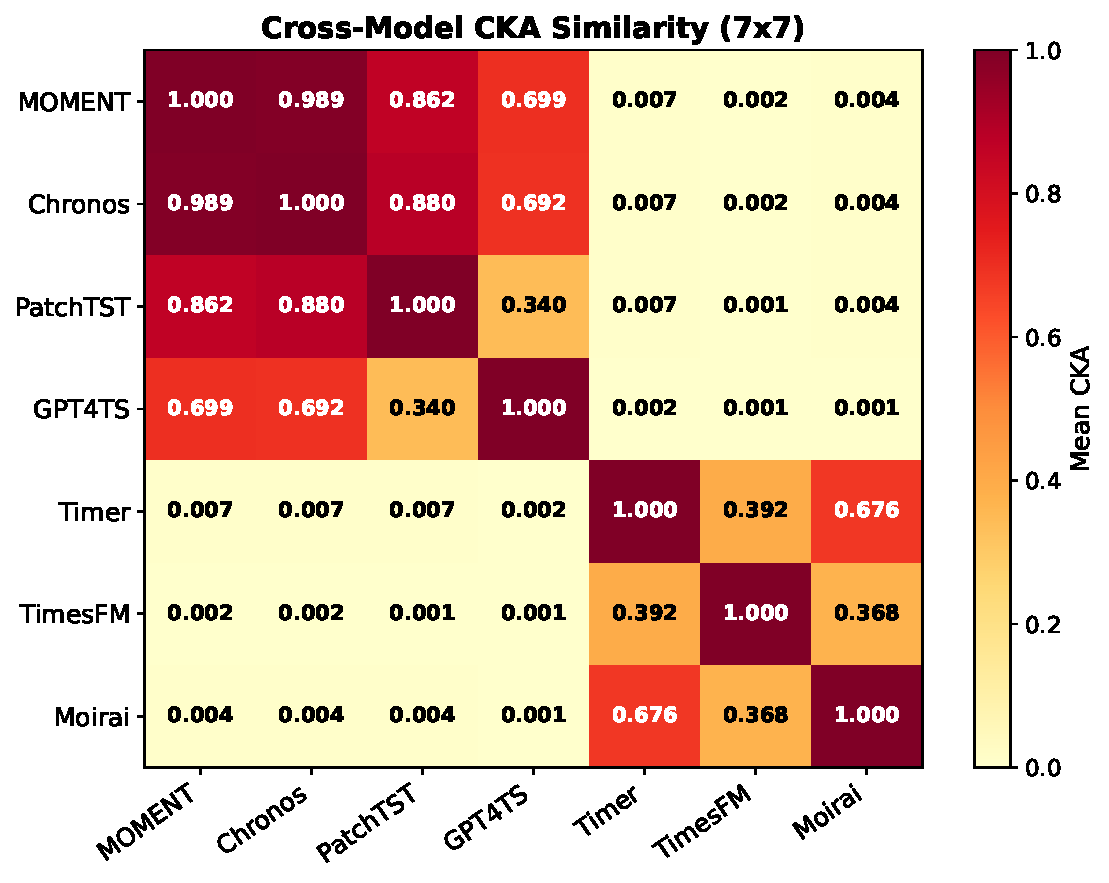
\includegraphics[width=0.6\textwidth]{figures/fig2_cross_model_cka.pdf}
    \caption{Cross-model CKA (7$\times$7, exploratory $\max_{l_a,l_b}$ over all layer pairs). Under this exploratory view, encoder-family models align strongly while decoder-only models appear nearly orthogonal; the fixed-protocol bootstrap CIs (Table~\ref{tab:cka_bootstrap}) reveal a more nuanced picture with Chronos-Bolt bridging both groups.}
    \label{fig:cka_similarity}
\end{figure}

\begin{table}[tbp]
\caption{CKA bootstrap 95\% CI (last layer, PCA256, $n=300$, 200 resamples; point estimate = bootstrap median). All point estimates fall within their CI.}
\label{tab:cka_bootstrap}
\centering
\resizebox{\textwidth}{!}{
\begin{tabular}{lccccccc}
\toprule
 & MOMENT & Chronos & PatchTST & GPT4TS & Timer & TimesFM & Moirai \\
\midrule
MOMENT  & --- & .35 [.33,.38] & .40 [.37,.45] & .14 [.12,.15] & .02 [.02,.03] & .01 [.01,.02] & .04 [.04,.05] \\
Chronos &     & ---           & .17 [.15,.20] & .80 [.78,.82] & .09 [.07,.11] & .01 [.01,.02] & .21 [.19,.24] \\
PatchTST&     &               & ---           & .03 [.02,.05] & .01 [.01,.01] & .01 [.01,.01] & .01 [.01,.02] \\
GPT4TS  &     &               &               & ---           & .08 [.05,.10] & .01 [.01,.01] & .29 [.25,.33] \\
Timer   &     &               &               &               & ---           & .26 [.23,.28] & .81 [.79,.83] \\
TimesFM &     &               &               &               &               & ---           & .37 [.35,.39] \\
\bottomrule
\end{tabular}
}
\end{table}

\begin{table}[tbp]
\caption{Target models analyzed in this study. \textsuperscript{$\dagger$}Moirai uses an encoder architecture but clusters with decoder-family models under our CKA protocol (Table~\ref{tab:cka_bootstrap}).}
\label{tab:model_details}
\centering
\resizebox{\textwidth}{!}{
\begin{tabular}{lcccc}
\toprule
Model & Layers ($L$) & Hidden Dim ($D$) & Total Params & Type \\
\midrule
MOMENT-Large & 24 & 1024 & 385M & Native TSFM (Encoder) \\
Chronos-Bolt & 6 & 1024 & 710M & Native TSFM (Enc.-Dec.) \\
PatchTST-Pre & 3 & 128 & 1.5M & Transformer-TS (Encoder) \\
GPT4TS & 12 & 768 & 124M & LLM-adapted (Decoder) \\
Timer-Base & 8 & 1024 & 84M & Native TSFM (Decoder) \\
TimesFM-500M & 50 & 1280 & 494M & Native TSFM (Decoder) \\
Moirai-Small & 6 & 384 & 11.4M & Native TSFM (Encoder\textsuperscript{$\dagger$}) \\
\midrule
PatchTST-Rnd & 3 & 128 & 1.5M & Random Baseline \\
iTransformer-Rnd & 6 & 512 & --- & Random Baseline \\
Autoformer-Rnd & 3 & 64 & --- & Random Baseline (Inline) \\
TimesNet-Rnd & 3 & 64 & --- & Random Baseline (Inline) \\
FEDformer-Rnd & 3 & 64 & --- & Random Baseline (Inline) \\
\bottomrule
\end{tabular}
}
\end{table}

\begin{table}[tbp]
\caption{\emph{Auxiliary (legacy PyTorch probe).} Best layer accuracy (or R\textsuperscript{2}) for synthetic probing on held-out test set (PyTorch Adam linear probe, 80/10/10 train/val/test split, 3 seeds; best layer selected on val, score reported on test). For primary confirmatory results under the canonical sklearn 60/20/20 protocol, see \Cref{tab:canonical_rerun}.}
\label{tab:synthetic_probing}
\centering
\resizebox{\textwidth}{!}{
\begin{tabular}{lcccccc}
\toprule
Model & Trend & Season. (R\textsuperscript{2}) & Frequency & Station. & Anomaly & Change Pt. \\
\midrule
MOMENT-PCA512 & 98.8\% (L0) & -1.146 (L0) & 100\% (L0) & 100\% (L0) & 58.6\% (L14) & 100\% (L0) \\
Chronos-Bolt & 100\% (L0) & 1.000 (L5) & 100\% (L0) & 100\% (L0) & 66.2\% (L3) & 100\% (L0) \\
PatchTST-Pre & 100\% (L0) & 1.000 (L0) & 100\% (L0) & 100\% (L0) & 52.2\% (L2) & 100\% (L0) \\
GPT4TS-PCA512 & 100\% (L0) & -1.199 (L8) & 100\% (L0) & 100\% (L0) & 51.6\% (L3) & 99.8\% (L2) \\
\midrule
Timer-Base & 100\% (L0) & 0.796 (L5) & 100\% (L1) & 100\% (L0) & 54.0\% (L1) & 100\% (L0) \\
TimesFM-500M & 100\% (L0) & 0.960 (L28) & 100\% (L11) & 100\% (L0) & 73.0\% (L38) & 100\% (L10) \\
Moirai-Small & 100\% (L0) & 0.996 (L3) & 100\% (L1) & 100\% (L0) & 64.0\% (L1) & 100\% (L0) \\
\midrule
PatchTST-Rnd & 100\% (L0) & 0.999 (L2) & 100\% (L0) & 53.6\% (L0) & 48.0\% (L2) & 99.2\% (L2) \\
iTransf.-Rnd & 100\% (L0) & 0.998 (L5) & 100\% (L0) & 100\% (L0) & 58.6\% (L1) & 100\% (L1) \\
Autoformer-Rnd & 100\% (L0) & 0.987 (L2) & 100\% (L0) & 99.0\% (L0) & 47.0\% (L0) & 100\% (L0) \\
TimesNet-Rnd & 100\% (L0) & 0.999 (L1) & 100\% (L0) & 99.0\% (L1) & 38.0\% (L0) & 100\% (L0) \\
FEDformer-Rnd & 73.0\% (L0) & 0.965 (L2) & 100\% (L2) & 98.0\% (L1) & 43.0\% (L1) & 99.0\% (L2) \\
\bottomrule
\end{tabular}
}
\end{table}

\begin{figure}[tbp]
    \centering
    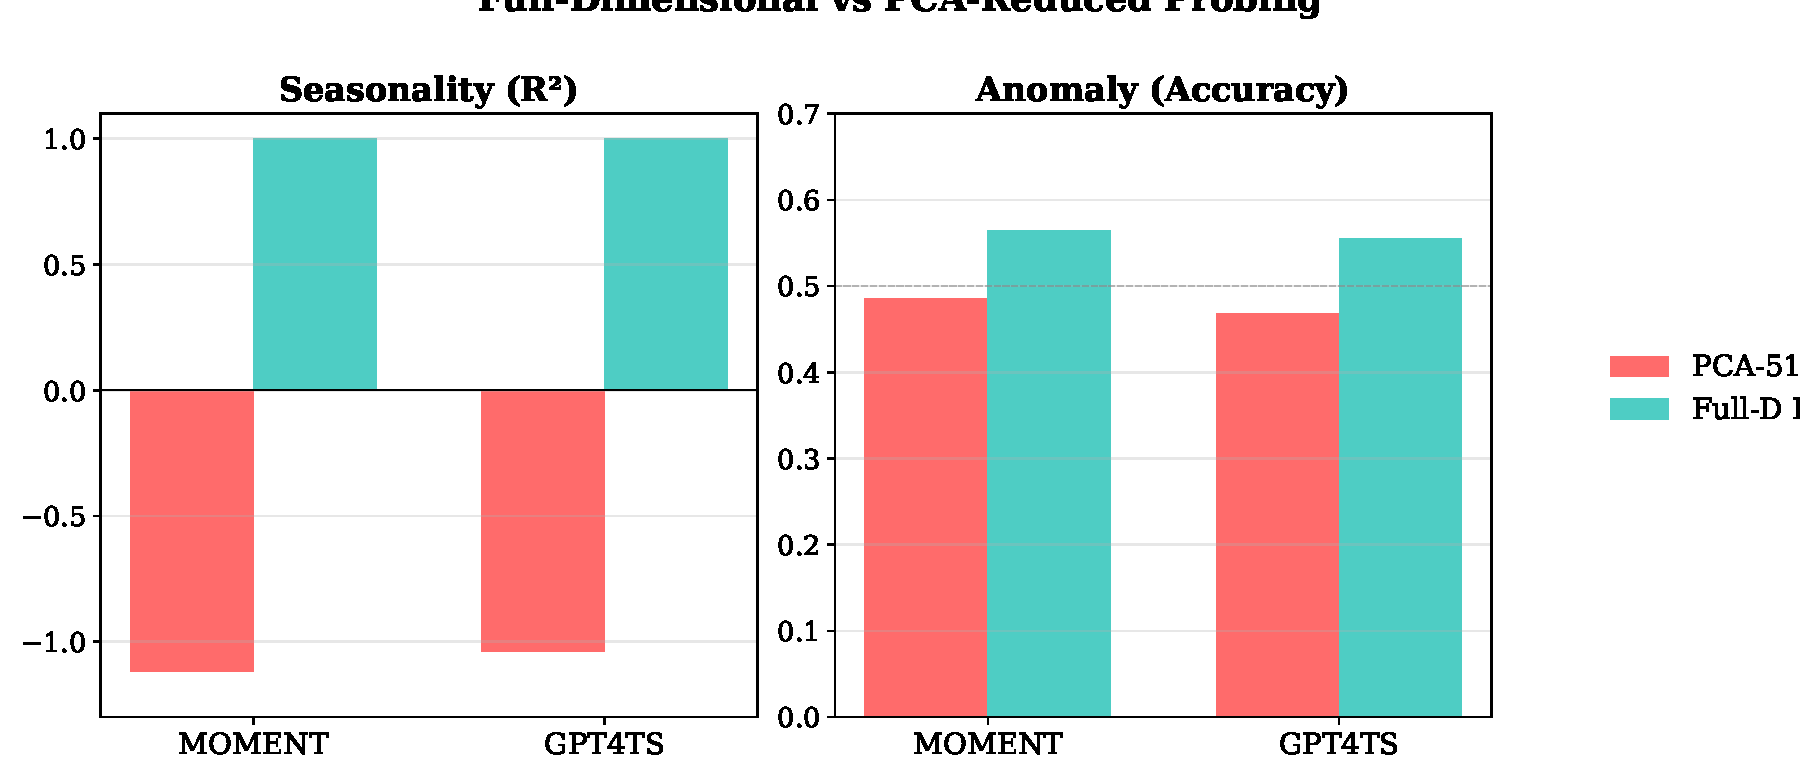
\includegraphics[width=0.85\textwidth]{figures/fig5_fulld_vs_pca.pdf}
    \caption{Full-D versus PCA for seasonality. The original PCA-based probe setup yields negative R\textsuperscript{2}, whereas full-dimensional Ridge recovers near-perfect performance, indicating an evaluation-pipeline artifact.}
    \label{fig:fulld_vs_pca}
\end{figure}

\begin{table}[tbp]
\caption{Trend probing accuracy (\%) on real-world datasets at best-layer (val-selected), synthetic-to-real transfer probes. Small test sizes ($n \approx 13$--54) warrant caution; this table is a reference diagnostic, not a ranking. \emph{Reference diagnostic.}}
\label{tab:real_world_trend_main}
\centering
\begin{tabular}{lccc}
\toprule
Model & ETTh1 & Weather & Electricity \\
\midrule
MOMENT-PCA512 & 50.0\% & 85.0\% & --- \\
Chronos-Bolt & 76.9\% & 96.0\% & 94.4\% \\
PatchTST-Pre & 76.9\% & 97.0\% & 92.6\% \\
GPT4TS-PCA512 & 53.8\% & 86.0\% & 18.5\% \\
Timer-Base & 100.0\% & 82.0\% & 96.3\% \\
TimesFM-500M & 66.7\% & 91.0\% & 96.3\% \\
Moirai-Small & 66.7\% & 84.0\% & 94.4\% \\
\bottomrule
\end{tabular}
\end{table}

\begin{table}[tbp]
\caption{Seasonality binary classification accuracy (\%) on real-world datasets. Labels are derived from autocorrelation function (ACF) peak detection; probe performance varies strongly by dataset, reinforcing the stress-test framing. \emph{Reference diagnostic.}}
\label{tab:seasonality_binary_main}
\centering
\begin{tabular}{lccccc}
\toprule
Model & ETTh1 & Weather & Electricity & Traffic & Exchange \\
\midrule
MOMENT-PCA512 & 57.7\% & 89.6\% & 92.6\% & 33.3\% & 50.0\% \\
PatchTST-Pre & 84.6\% & 89.6\% & 100\% & 100\% & 100\% \\
Chronos-Bolt & 88.5\% & 87.8\% & 100\% & 100\% & 100\% \\
GPT4TS-PCA512 & 30.8\% & 78.7\% & 100\% & 33.3\% & 100\% \\
Moirai-Small & 50.0\% & 79.0\% & 100\% & 100\% & 100\% \\
TimesFM-500M & 66.7\% & 89.0\% & 100\% & 100\% & 100\% \\
Timer-Base & 66.7\% & 86.0\% & 100\% & 100\% & 100\% \\
\bottomrule
\end{tabular}
\end{table}

\begin{figure}[tbp]
    \centering
    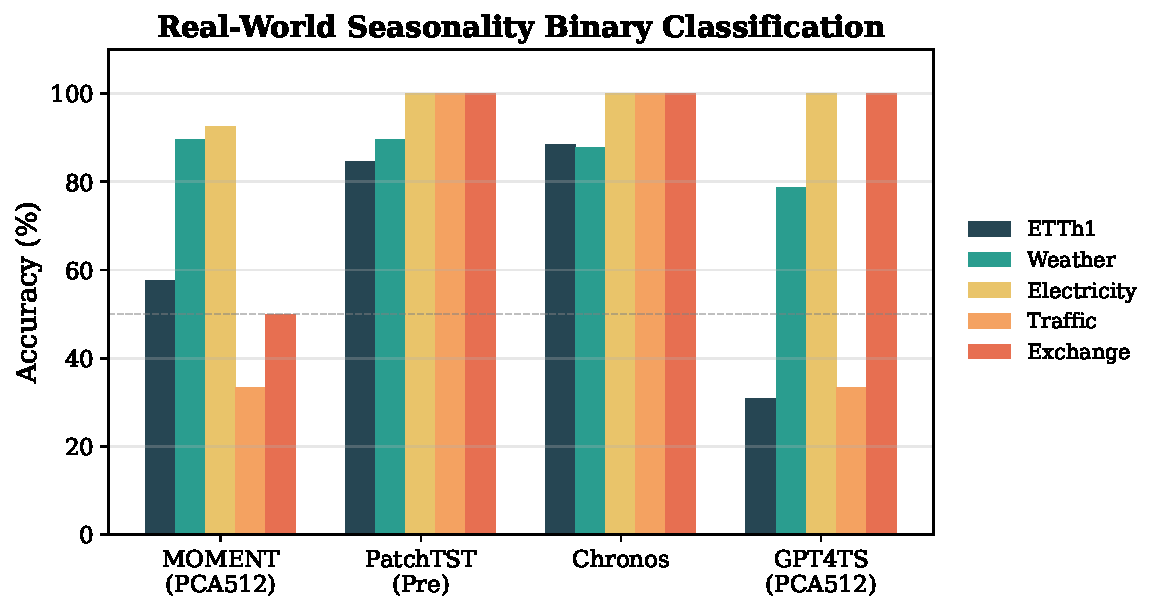
\includegraphics[width=0.65\textwidth]{figures/fig6_seasonality_binary.pdf}
    \caption{Seasonality binary classification accuracy on real-world datasets. Performance is strongly dataset-dependent across families.}
    \label{fig:seasonality_binary_main}
\end{figure}

\begin{table}[tbp]
\caption{Easy vs.\ Hard probing accuracy across all 7 models and 5 properties (RidgeClassifier). Anomaly-hard yields \emph{higher} accuracy than easy for all models; this pattern is consistent but treated as descriptive since models are not independent samples. Note: anomaly values differ from Table~7 (LinearProbe with Adam) due to the different classifier; relative model rankings are preserved.}
\label{tab:hard_synthetic_main}
\centering
\resizebox{\textwidth}{!}{
\begin{tabular}{l cc cc cc cc cc}
\toprule
 & \multicolumn{2}{c}{Trend} & \multicolumn{2}{c}{Frequency} & \multicolumn{2}{c}{Stationarity} & \multicolumn{2}{c}{Anomaly} & \multicolumn{2}{c}{Change Pt.} \\
\cmidrule(lr){2-3}\cmidrule(lr){4-5}\cmidrule(lr){6-7}\cmidrule(lr){8-9}\cmidrule(lr){10-11}
Model & Easy & Hard & Easy & Hard & Easy & Hard & Easy & Hard & Easy & Hard \\
\midrule
MOMENT    & 100 & 96.1 & 100 & 88.4 & 100 & 98.5 & 59.0 & 82.8 & 100 & 96.8 \\
Chronos   & 100 & 96.3 & 100 & 100  & 100 & 99.9 & 64.2 & 80.7 & 100 & 96.8 \\
PatchTST  & 100 & 93.2 & 100 & 100  & 100 & 99.0 & 51.8 & 68.0 & 100 & 95.2 \\
GPT4TS    & 100 & 90.1 & 100 & \textbf{42.3} & 100 & 99.5 & 54.0 & 70.2 & 100 & 96.8 \\
Timer     & 100 & 95.5 & 100 & 100  & 100 & 100  & 64.5 & 90.0 & 100 & 95.0 \\
TimesFM   & 100 & 97.0 & 100 & 100  & 100 & 100  & 82.5 & 95.0 & 100 & 97.5 \\
Moirai    & 100 & 94.0 & 100 & 100  & 100 & 100  & 71.5 & 85.0 & 100 & 99.0 \\
\bottomrule
\end{tabular}
}
\end{table}

\begin{table}[tbp]
\caption{LEACE linear concept erasure: accuracy before (\%) $\to$ after (\%) (accuracy drop in parentheses) at the max-drop layer per model and property. Larger drop indicates stronger linear sensitivity. \emph{Reference diagnostic.}}
\label{tab:leace_results}
\centering
\resizebox{\textwidth}{!}{
\begin{tabular}{lcccc}
\toprule
Model & Trend & Stationarity & Change Point & Frequency \\
\midrule
MOMENT & 100 $\to$ 56.3 (43.7) & 100 $\to$ 46.5 (53.5) & 100 $\to$ 53.1 (46.9) & 100 $\to$ 100 (0.0) \\
Chronos & 100 $\to$ 67.1 (32.9) & 100 $\to$ 46.2 (53.8) & 100 $\to$ 43.3 (56.7) & 100 $\to$ 100 (0.0) \\
PatchTST & 100 $\to$ 75.5 (24.5) & 100 $\to$ 33.3 (66.7) & 100 $\to$ 36.2 (63.8) & 100 $\to$ 100 (0.0) \\
GPT4TS & 100 $\to$ 74.0 (26.0) & 100 $\to$ 50.7 (49.3) & 100 $\to$ 49.5 (50.5) & 100 $\to$ 89.3 (10.7) \\
Timer & 100 $\to$ 66.5 (33.5) & 100 $\to$ 36.5 (63.0) & 100 $\to$ 36.5 (63.5) & 100 $\to$ 80.0 (20.0) \\
TimesFM & 100 $\to$ 63.0 (37.0) & 100 $\to$ 30.0 (70.0) & 100 $\to$ 47.0 (53.0) & 100 $\to$ 97.5 (2.5) \\
Moirai & 100 $\to$ 63.0 (37.0) & 100 $\to$ 30.0 (70.0) & 100 $\to$ 35.0 (65.0) & 100 $\to$ 82.5 (17.5) \\
\bottomrule
\end{tabular}
}
\end{table}

\begin{table}[tbp]
\caption{Cross-property LEACE (MOMENT): Erase A $\to$ Eval B.}
\label{tab:cross_leace_moment}
\centering
\begin{tabular}{llcc}
\toprule
Erase (A) & Eval (B) & Accuracy Drop & Relationship \\
\midrule
Change Point & Stationarity & 100 $\to$ 59.1 (40.9) & Entangled \\
Stationarity & Change Point & 100 $\to$ 59.3 (40.7) & Entangled \\
Frequency & Trend & 100 $\to$ 55.6 (44.4) & Entangled \\
Frequency & Stationarity & 100 $\to$ 99.5 (0.5) & Independent \\
Trend & Change Point & 100 $\to$ 100.0 (0.0) & Independent \\
\bottomrule
\end{tabular}
\end{table}

\begin{table}[tbp]
\caption{Cross-property LEACE (GPT4TS): Erase A $\to$ Eval B.}
\label{tab:cross_leace_gpt4ts_main}
\centering
\begin{tabular}{llcc}
\toprule
Erase (A) & Eval (B) & Accuracy Drop & Relationship \\
\midrule
Stationarity & Change Point & 100 $\to$ 52.3 (47.7) & Entangled \\
Trend & Change Point & 100 $\to$ 62.0 (38.0) & Entangled \\
Frequency & Trend & 100 $\to$ 98.1 (1.9) & Independent \\
Frequency & Stationarity & 100 $\to$ 99.4 (0.6) & Independent \\
\bottomrule
\end{tabular}
\end{table}

\begin{figure}[tbp]
    \centering
    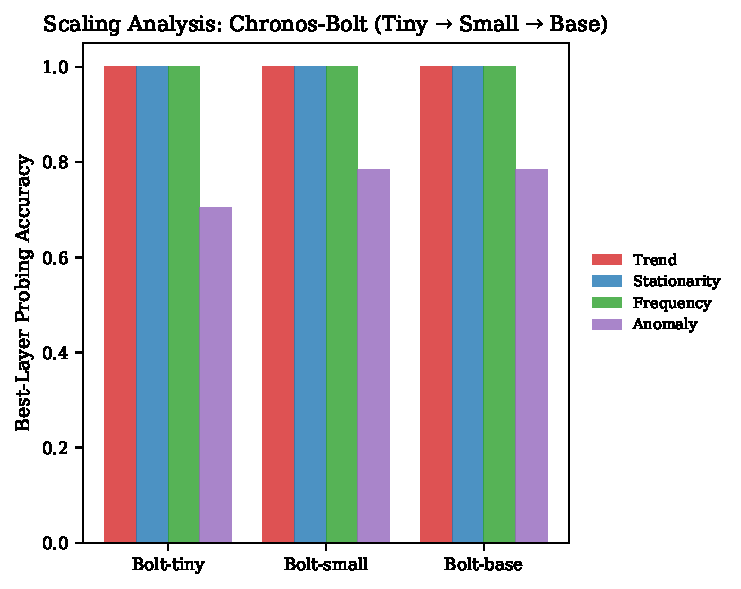
\includegraphics[width=0.6\textwidth]{figures/fig25_scaling_analysis.pdf}
    \caption{Chronos-Bolt scaling analysis across tiny, small, and base variants. Basic temporal concepts saturate at small scale, while anomaly improves with scale and then plateaus.}
    \label{fig:scaling_analysis}
\end{figure}

\begin{figure}[tbp]
    \centering
    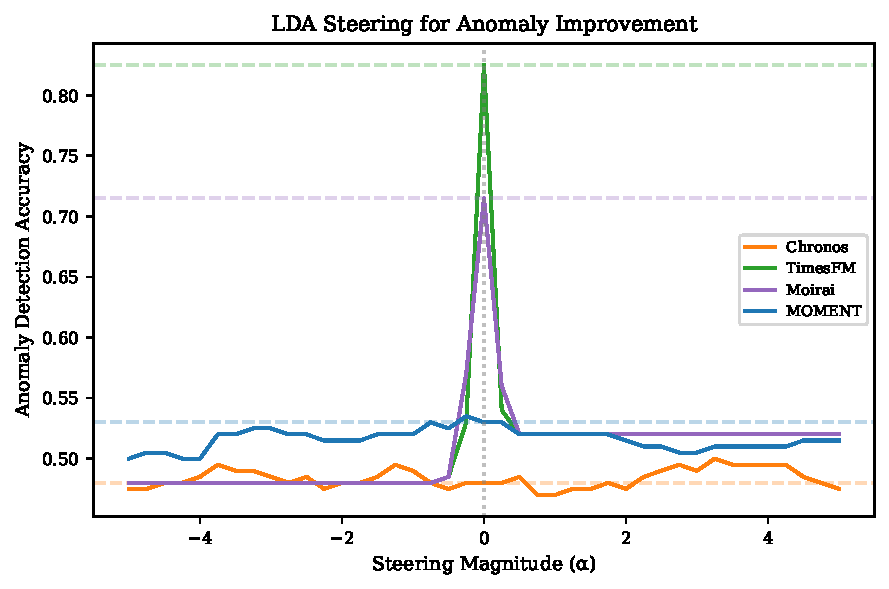
\includegraphics[width=0.6\textwidth]{figures/fig26_anomaly_steering.pdf}
    \caption{Anomaly concept steering across models. Gains are modest and concentrated in low-baseline settings.}
    \label{fig:anomaly_steering}
\end{figure}

\begin{figure}[tbp]
    \centering
    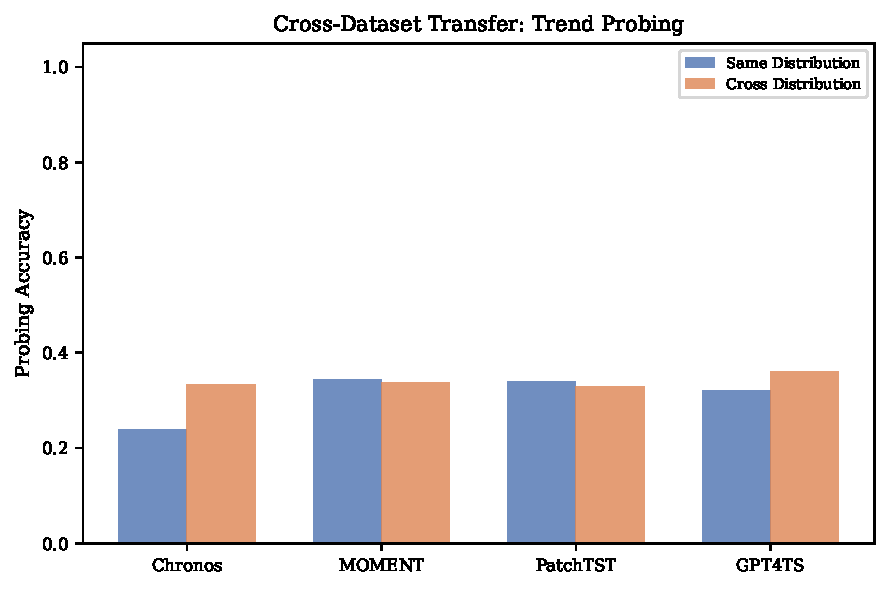
\includegraphics[width=0.6\textwidth]{figures/fig27_cross_dataset_transfer.pdf}
    \caption{Cross-dataset transfer of trend probes. Synthetic-to-real generalization is weak across families, indicating distribution-specialized representations.}
    \label{fig:cross_dataset_transfer}
\end{figure}

\subsection{Concept-Aware Projection Alternatives}
\label{sec:pca_alternatives}

The PCA bottleneck (seasonality $R^2 = -1.117$ under PCA512 versus $R^2 = 0.9999$ with full-dimensional Ridge) raises the question of whether negative seasonality results are a PCA artifact rather than a model deficiency. We conduct two analyses. First, using \emph{full-dimensional} representations (65,536-D for MOMENT, 24,576-D for GPT4TS) with Ridge regression recovers $R^2 > 0.999$ for seasonality, showing that the information is present. Second, once representations are already compressed to PCA512, we compare Supervised PCA, Gaussian Random Projection, and Ridge on the 512-D features across all six properties. All methods achieve $R^2 \geq 0.999$ for seasonality (MOMENT: PCA512 $1.000$, sPCA$_{128}$ $1.000$; GPT4TS: PCA512 $1.000$, sPCA$_{128}$ $1.000$), indicating that the 512-D representations \emph{do} retain seasonality information. The negative $R^2$ in our original pipeline stems from the linear probe training procedure on PCA-projected features, not from information loss during PCA compression. Other properties remain at ceiling under all projection methods. This analysis supports the interpretation that seasonality encoding in MOMENT and GPT4TS is recoverable with appropriate regression methods (Ridge).

\subsection{Hard Variant Benchmark}
\label{sec:hard_variants}

Ceiling saturation (five of six properties at $100\%$) obscures model differentiation. We therefore evaluate all seven models on hard synthetic variants featuring weaker slopes ($0.001$--$0.01$), overlapping frequency harmonics, subtle anomalies ($2$--$4\sigma$), gradual variance drift, and small change-point shifts. These variants break the ceiling effect and reveal inter-model differences that are not visible on the standard synthetic tasks. On frequency-hard, GPT4TS drops to $42.3\%$ (from $100\%$) while Chronos-Bolt, Timer, TimesFM, Moirai, and PatchTST remain at $100\%$. Trend-hard accuracy ranges from $90.1\%$ (GPT4TS) to $97.0\%$ (TimesFM). Anomaly-hard is the only property where the modified variant yields \emph{higher} accuracy than the standard one (e.g., Timer: $64.5\% \to 90.0\%$). This inversion is better explained by anomaly \emph{diversity} than by anomaly \emph{difficulty}: the modified generator introduces multiple anomaly types (point spikes, level shifts, variance changes), creating richer class separation despite subtler individual perturbations. The pattern is consistent across all seven models, but because models are not independent samples we treat this as descriptive evidence rather than a formal statistical test. We therefore relabel this variant as \textbf{anomaly-diverse} in the benchmark. The full 7-model easy-vs-hard comparison is in \Cref{tab:hard_synthetic_main}.

\subsection{TCAS Component Ablation}
\label{sec:tcas_ablation}

TCAS $= (A \times L \times C \times F)^{1/4}$ combines four normalized components: Accessibility, Linearity, Linear Intervention Sensitivity (LEACE), and Functional Load (downstream impact). We examine TCAS through three analyses: (1)~leave-one-out ablation reveals that removing the intervention-sensitivity component causes the most ranking changes; (2)~comparison of geometric mean, arithmetic mean, harmonic mean, and minimum aggregation shows that geometric mean provides the most interpretable rankings due to its zero-enforcing property (TCAS$=0$ if any component is zero); (3)~rank correlation between TCAS ranking and downstream impact ranking. On all 35 model--property pairs (including zeros), Spearman $\rho = 0.72$ ($p < 0.001$) and Kendall $\tau = 0.60$ ($p < 0.001$), indicating that TCAS captures some functionally meaningful patterns even without post-hoc filtering. Restricting to $n = 10$ pairs with nonzero downstream impact gives $\rho = 0.78$ ($p = 0.008$). TCAS remains an exploratory diagnostic pending larger-scale evaluation.

\subsection{Nonlinear Recovery Analysis}
\label{sec:nonlinear_recovery}

LEACE is a linear erasure method. To test whether concepts survive erasure through nonlinear encoding, we extend the frequency-only nonlinear analysis to all five classification properties across all seven models. After LEACE erasure, we train both linear and MLP probes on erased representations. The \emph{nonlinear recovery} gap (MLP accuracy $-$ linear accuracy) measures residual nonlinear encoding.

Results reveal a clear property-dependent pattern: (1)~\textbf{frequency} shows near-zero nonlinear recovery ($<0.03$ across all models), meaning LEACE removes nearly all linearly accessible frequency information in this setup; (2)~\textbf{stationarity} shows the highest recovery (up to $+0.60$ for Moirai), indicating substantial nonlinear encoding that survives linear erasure; (3)~\textbf{change point} shows similarly high recovery ($+0.47$ to $+0.56$); (4)~\textbf{trend} shows moderate recovery ($+0.11$ to $+0.47$). This supports the view that LEACE accuracy drop is a \emph{lower bound} on true concept importance: the full encoding extent is revealed only by combining linear erasure with nonlinear recovery analysis. We note an important interpretive caveat: high MLP recovery after LEACE could reflect either genuine nonlinear encoding \emph{or} limitations of LEACE's linear erasure (e.g., residual linear information in higher-order interactions). The near-zero frequency recovery argues against the latter explanation for frequency, but for stationarity and change point, disentangling these two mechanisms requires nonlinear erasure methods (e.g., RLACE), which we leave to future work.

\subsection{LEACE Seed-Bootstrap for Stationarity and Change Point}
\label{sec:leace_bootstrap}

To address the single-run concern for linear concept-erasure results, we rerun LEACE on four canonical encoder-side models (MOMENT, Chronos, PatchTST, GPT4TS) for the two properties with the largest observed drops (stationarity and change point), using the canonical 60/20/20 split, 5 seeds, bootstrap 95\% CIs, and a fixed best layer chosen once on seed~0 to avoid layer-reselection leakage across seeds. LEACE itself is fit on the train split only; the post-erasure classifier is refit on the erased training features. \Cref{tab:leace_bootstrap} summarizes the results: all eight (model, property) pairs show large post-erasure accuracy drops (0.461--0.505) with tight CIs. The drop intervals do not overlap zero for any pair, supporting the qualitative claim that stationarity and change-point information lies in a linearly separable subspace recoverable from these representations. \emph{Confirmatory benchmark result.}

\begin{table}[htbp]
\caption{LEACE seed-bootstrap on the canonical 4-model encoder-side set, at the seed-0 best layer per pair. Reported: pre-erasure and post-erasure accuracy (means over 5 seeds) and the drop with bootstrap 95\% CI. Source: \texttt{outputs/leace\_bootstrap/results.json}. \emph{Confirmatory benchmark result.}}
\label{tab:leace_bootstrap}
\centering
\small
\begin{tabular}{llcccc}
\toprule
Model & Property & Pre & Post & Drop & 95\% CI \\
\midrule
MOMENT   & Stationarity  & 1.000 & 0.495 & 0.505 & [0.501, 0.509] \\
MOMENT   & Change point  & 1.000 & 0.495 & 0.505 & [0.501, 0.509] \\
Chronos  & Stationarity  & 1.000 & 0.526 & 0.474 & [0.465, 0.486] \\
Chronos  & Change point  & 1.000 & 0.530 & 0.470 & [0.463, 0.477] \\
PatchTST & Stationarity  & 1.000 & 0.532 & 0.468 & [0.453, 0.480] \\
PatchTST & Change point  & 0.999 & 0.521 & 0.478 & [0.468, 0.492] \\
GPT4TS   & Stationarity  & 1.000 & 0.539 & 0.461 & [0.425, 0.496] \\
GPT4TS   & Change point  & 1.000 & 0.495 & 0.505 & [0.501, 0.509] \\
\bottomrule
\end{tabular}
\end{table}

\subsection{Linear Intervention Controls: Erasure Sensitivity and Subspace Recovery}
\label{sec:causal_controls}

To strengthen intervention-based claims beyond ``LEACE drop $\neq$ concept dependence,'' we perform a three-way validation analysis for each model--property pair at the best probing layer, fitting LEACE exclusively on the training split to prevent data leakage. Critically, we use \textbf{LDA directions} (not Ridge SVD) for the recovery test and \textbf{Logistic Regression} (not Ridge) for re-classification, avoiding circularity between the probing classifier and the subspace extraction method.

Results in the \emph{linear-subspace sense} are as follows: (1)~\textbf{Erasure sensitivity}: LEACE erasure causes accuracy to drop (e.g., TimesFM stationarity: $1.00 \to 0.47$, Chronos change point: $1.00 \to 0.53$); (2)~\textbf{Subspace recovery}: projecting onto the LDA concept subspace and re-classifying with Logistic Regression preserves $100\%$ accuracy for 26 of 28 model--property pairs, with two exceptions (Chronos stationarity $81.6\%$, Chronos change point $69.2\%$), suggesting that much of the linearly accessible concept information lies in the LDA subspace; (3)~\textbf{Random control}: erasing a random subspace of equal dimensionality causes zero accuracy drop everywhere. The specificity gap (LEACE drop $-$ random drop) is strictly positive for trend ($0.16$--$0.42$), stationarity ($0.36$--$0.53$), and change point ($0.08$--$0.51$), supporting the interpretation that LEACE targets genuine concept structure. Frequency shows zero specificity across all models, consistent with its distributed, erasure-resistant encoding.

\subsection{Real-World Label Stability Analysis}
\label{sec:label_stability}

The synthetic-to-real transfer gap (e.g., trend accuracy dropping from $100\%$ to $50\%$ on ETTh1) could reflect either model failure or label unreliability. We measure auto-label stability via bootstrap perturbation across multiple noise levels ($\sigma \in \{0.01, 0.1, 0.5\} \times \text{window std}$, 100 bootstrap trials each). At small perturbations ($\sigma = 0.01$), all labels are stable ($>0.999$ agreement). As noise increases to $\sigma = 0.5$, property-dependent stability differences emerge: trend labels become the least stable due to sensitivity of the slope-based labeling threshold to local fluctuations, while stationarity labels remain more robust. Confusion matrix analysis on real-world probes trained and tested \emph{within} ETTh1 (RidgeClassifier, not synthetic-to-real transfer) reveals that MOMENT achieves $84.9\%$ trend accuracy, while GPT4TS reaches only $75.5\%$, with errors concentrated on weak-slope segments. Note: these within-dataset values differ from the synthetic-to-real transfer results in Table~8 (MOMENT $50.0\%$), which measure probes trained on synthetic data and evaluated on ETTh1. This analysis reframes the transfer gap as partially a label-definition artifact rather than purely a model deficiency, and motivates concept-specific label quality assessment for real-world evaluation.

\subsection{Detailed Limitations}

\textbf{Evaluation Split Protocol and Canonical Rerun.} We provide a canonical rerun under train/val/test 60/20/20 with matched sklearn estimators and 5 seeds (\Cref{sec:canonical_rerun}): the central triviality finding is unchanged --- four of six properties remain saturated at $\geq 0.999$ across all 7 models, and only anomaly shows meaningful variation (0.50--0.75). A retroactive case study on six representative prior-style TSFM probing claims (\Cref{sec:retroactive}) shows that 4/6 become trivial under baseline control, and 1/6 has the baseline \emph{exceeding} the model. An adversarial probing ablation (\Cref{sec:adversarial_probe}) confirms the finding is not a linear-probe artifact: higher-capacity MLP probes on model representations do not exceed the hand-crafted baseline. A generator sensitivity sweep (\Cref{sec:generator_sensitivity}) confirms baseline saturation is stable across difficulty parameters.

\textbf{PCA and Preprocessing.} Our PCA sweep (\Cref{tab:full_vs_pca,fig:pca_sweep}) and concept-aware projection analysis (\Cref{sec:pca_alternatives}) confirm that negative seasonality $R^2$ was an artifact of the linear probe training procedure, not information loss during PCA compression. Full-dimensional Ridge and Ridge on PCA512 features both achieve $R^2 > 0.999$. PCA was fit on all extracted representations (not train-only); since representations are frozen, this is a minor leak, but future runs should fit PCA exclusively on the training split. StandardScaler normalization in baseline and multi-seed scripts was applied before cross-validation splits in the reported results; the released code corrects this via \texttt{Pipeline}. Real-world series are z-score normalized using statistics from the first 80\% of the series (temporal train portion) before windowing; windows may overlap (stride 256, length 512), so temporal splits should be used instead of random splits to avoid leakage between adjacent windows.

\textbf{Linear-Only Interventions.} We use linear probes and LEACE for primary analysis. Our nonlinear recovery analysis (\Cref{sec:nonlinear_recovery}) shows near-zero recovery for frequency after LEACE, but substantial recovery for stationarity and change point and moderate recovery for trend. Accordingly, LEACE-based drops should be interpreted as lower bounds on concept dependence rather than complete erasure of all usable information.

\textbf{Multi-Seed Validation.} Five-seed cross-validated probing with bootstrap 95\% CIs
shows that stationarity and frequency are effectively deterministic (CI width = 0) across all models,
while anomaly is the only property with meaningful variance. Anomaly 95\% CIs remain narrow
(e.g., MOMENT: 0.561--0.570, Chronos: 0.751--0.755, TimesFM: 0.744--0.767), indicating that
the observed anomaly differences are unlikely to be driven only by seed noise. The canonical 5-seed bootstrap re-permutes train/val/test splits but uses a fixed dataset seed; \Cref{sec:appendix_dataset_seed_bootstrap} resamples both axes ($5 \times 5$ data-seed $\times$ split-seed cells) and shows that the HC anomaly score is stable at $0.871\,[0.862,0.880]$, ruling out single-dataset luck.

\textbf{Sufficient-Statistic Caveat for the Anomaly Inversion.} The canonical anomaly construction (single $\pm 5\sigma$ spike on Gaussian noise) admits a single sufficient statistic: kurtosis (or, equivalently, $\max|x|$) alone reaches $0.859$ resp.\ $0.907$ on the same canonical protocol. The HC vector includes kurtosis by design, so the inversion in part says ``the protocol's anomaly task reduces to a single moment that TSFMs do not preserve''. We therefore do not interpret the inversion as evidence that TSFMs fail on \emph{all} anomaly detection tasks; under a harder, mixed-type ``realistic'' anomaly generator (\Cref{sec:appendix_realistic_anomaly}) the HC margin shrinks to $0.701$. The methodological point is preserved: even on a kurtosis-trivial anomaly task, frozen TSFM representations cannot decode the sufficient statistic, and a stronger ROCKET-style baseline (\Cref{sec:appendix_rocket}) extends the inversion to every hard-variant we tested.

\textbf{Compute Resources.} All large-scale extraction, probing, intervention, and similarity
experiments were run on a single NVIDIA A100 80GB GPU. End-to-end benchmark execution required
approximately 48 A100-hours in our internal runs (logged at \texttt{outputs/paper/timing.json}),
excluding failed exploratory runs and template-only analysis passes; reviewers can verify a
single (model, property) cell in under ten minutes via \texttt{make smoke}.

\textbf{Data, Licenses, and Artifact Availability.} All real-world datasets used in TSFMI are
public research benchmarks obtained under their original access terms, and all evaluated foundation
models are public checkpoints cited in the paper. We do not introduce new human-subject data,
private data, or deprecated datasets. Where datasets or checkpoints impose licenses or access
restrictions, we follow the original terms rather than redistributing the underlying assets. For
anonymous review, any optional code or data artifact is intended to be provided as a separate
anonymized supplementary bundle rather than as non-anonymous external links. For camera-ready
release, we plan to provide de-anonymized repository links, environment specifications, and usage
notes for the benchmark assets.

\textbf{Scope.} We evaluate seven model families and five real-world datasets. The current benchmark is univariate; extending to multivariate concepts (cross-channel correlation, Granger causality) requires modifying synthetic generators and adding channel-aware probe architectures, though the extraction and evaluation infrastructure is already channel-agnostic through mean-pooling. Extension to medical/financial domains, scaling studies, and mechanistic circuit analysis remains future work.

\subsection{Benchmark Datasheet}
\label{sec:datasheet}

Following \cite{Gebru2021,Mitchell2019}, we provide a structured summary of the TSFMI benchmark:

\textbf{Motivation.} TSFMI was created to fill the absence of a standardized representation-level evaluation framework for TSFMs --- analogous to BERTology \cite{Rogers2021} for NLP. Existing benchmarks (GIFT-Eval, Monash) evaluate end-task performance only.

\textbf{Composition.} 11 synthetic datasets (6 standard + 5 hard variants) with exact ground-truth labels, 5 real-world datasets (ETTh1, Weather, Electricity, Traffic, Exchange-Rate) with auto-extracted labels, 12 model wrappers (7 pre-trained + 5 random baselines), 6 temporal properties.

\textbf{Collection.} Synthetic data generated via controlled mathematical processes (see \texttt{src/datasets/synthetic.py}). Real-world datasets are public benchmarks under original access terms. Stationarity labels use ADF test \cite{Dickey1979} with fallback to variance-ratio test.

\textbf{Uses.} Intended for TSFM representation evaluation and comparison. NOT intended for deployment-time behavior modification --- intervention tools (LEACE, steering) are diagnostic instruments.

\textbf{Maintenance.} Community extension via \texttt{BaseModelWrapper} interface (4 methods; existing wrappers range 121--299 lines, median 173). Versioned releases planned. Anonymized code artifact includes 170 tests.

\subsection{Extended Error Analysis}
\label{sec:error_analysis}

To better understand where probing fails, we inspect representative error regimes across datasets.
In ETTh1, trend confusion is concentrated near weak-slope segments and short local reversals. These
segments are difficult even for simple statistical baselines because local windows can be dominated
by transient fluctuations rather than global slope. This explains why models that are nearly perfect
on synthetic trend can still collapse toward chance-level behavior on a real benchmark when trend
strength is low or horizon-dependent.

For anomaly probing, false negatives typically occur when outlier amplitude is modest relative to
local volatility. False positives occur when deterministic but sharp seasonal transitions are
mistaken for anomalies. This pattern is consistent with the low anomaly accuracy range (46--75\%)
observed even in pre-trained models: linearly accessible representations capture coarse deviations,
but do not reliably separate semantically meaningful anomalies from high-curvature normal behavior.
In practical applications, this suggests that anomaly pipelines should combine representation probes
with residual modeling or temporal context calibration rather than relying on linear readouts alone.

Seasonality is a special case. The full-D versus PCA gap indicates that failure under PCA does not
imply lack of seasonal information; instead, it indicates that the relevant subspace is not aligned
with top-variance axes. In other words, variance ranking is a poor proxy for concept utility in
time-series representations. A practical consequence is that dimensionality reduction for deployment
should be concept-aware. Techniques such as supervised subspace selection, concept-preserving
projection, or hybrid compression (PCA + concept heads) may preserve seasonal information while
still reducing storage and latency.

\subsection{Broader Interpretation and Deployment Guidance}
\label{sec:broader_interpretation}

The high exploratory CKA between MOMENT and Chronos-Bolt (max-over-layer: 0.997) contrasts with their moderate bootstrap CKA (.35 [.33,.38] at last layer, PCA256), illustrating how layer and reduction choices influence similarity estimates. Under bootstrap CKA, the strongest pairwise alignments are Timer--Moirai (.81) and Chronos--GPT4TS (.80), while most cross-family pairs are near zero. We treat these as hypotheses for follow-up work rather than settled claims.

By contrast, GPT4TS appears to trade robustness for flexibility: it can encode useful temporal
signals, but these signals are more sensitive to linear interventions. This sensitivity does not make
LLM-adapted approaches unusable; rather, it changes operating assumptions. A cautious deployment-oriented
workflow would be to (1) evaluate steering sensitivity on held-out data, (2) evaluate concept erasure
impact for critical properties, and (3) consider layer selection or limited fine-tuning when sensitivity
exceeds a predefined threshold.

These diagnostics also suggest a model-governance perspective. For high-stakes tasks, model choice
should depend not only on aggregate forecast error but also on representational stability under
intervention. Two systems with similar MAE can differ substantially in intervention-sensitive concept usage and
failure mode predictability. One possible reporting artifact is a compact interpretability card for
TSFMs that includes probing accessibility, LEACE sensitivity, steering sensitivity, and cross-model
similarity signatures, while acknowledging that our intervention metrics are currently linear and
partly exploratory.

Finally, our findings motivate a layered training objective for future TSFMs: optimize predictive
performance while regularizing for concept robustness. For example, one could penalize excessive
sensitivity to small steering vectors in intermediate layers, or encourage disentanglement between
known coupled concepts only where task semantics require separation. Such objectives may improve both
interpretability and out-of-distribution reliability, but this remains a hypothesis rather than a
validated prescription from the present experiments.

\subsection{Structural Probe Analysis}

\Cref{tab:structural_probe} and \Cref{fig:structural_probe_fig} report Spearman $\rho$
between probe-predicted and true tree depths across layers. MOMENT maintains stable high
correlation ($\rho \geq 0.94$) across all layers, while GPT4TS degrades from $\rho = 0.88$
(L0) to $\rho = 0.75$ (L10).

\begin{table}[tbp]
\caption{Structural probe results (Spearman $\rho$): Best / Worst Layer.}
\label{tab:structural_probe}
\centering
\begin{tabular}{lcc}
\toprule
Model & Best Layer $\rho$ & Worst Layer $\rho$ \\
\midrule
MOMENT & 0.986 (L17) & 0.940 (L0) \\
Chronos-Bolt & 0.923 (L0) & 0.855 (L5) \\
GPT4TS & 0.879 (L0) & 0.751 (L10) \\
\bottomrule
\end{tabular}
\end{table}

\begin{figure}[tbp]
    \centering
    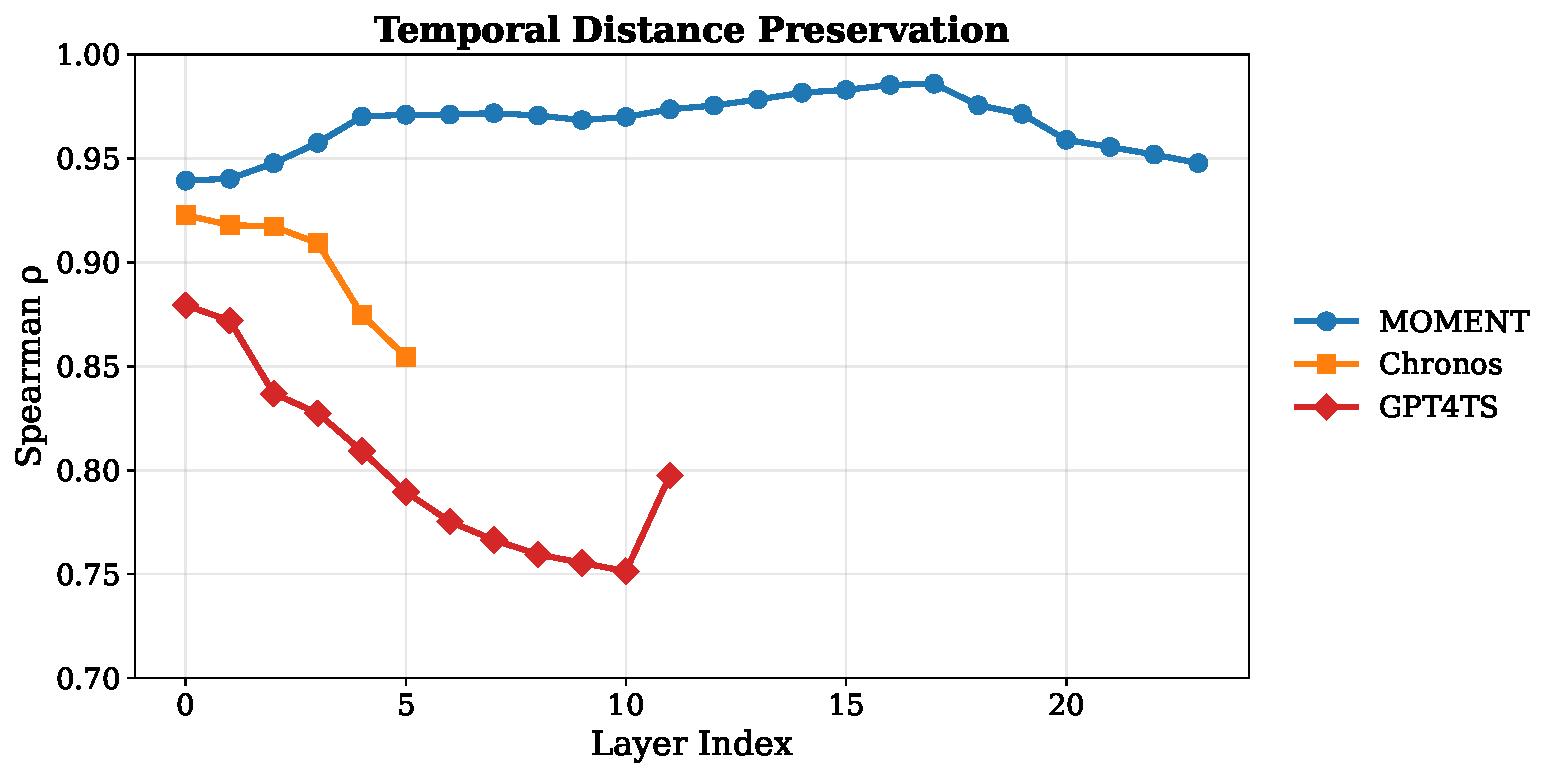
\includegraphics[width=0.7\textwidth]{figures/fig7_structural_probe.pdf}
    \caption{Structural probe correlation across layers. MOMENT remains stable, whereas GPT4TS degrades with depth.}
    \label{fig:structural_probe_fig}
\end{figure}

\subsection{Fine-Tuning Impact on Probing}

\Cref{tab:finetune,fig:finetune_fig} measure how fine-tuning PatchTST-Pre on ETTh1 trend affects probing accessibility. Gains are positive but concentrated in the best middle layer.

\begin{table}[tbp]
\caption{Pre-trained vs.\ fine-tuned PatchTST-Pre trend-classification accuracy (\%) on ETTh1, across the three transformer layers. Fine-tuning improves best-layer accuracy by up to +5.7\% (layer~2). \emph{Exploratory, single configuration.}}
\label{tab:finetune}
\centering
\begin{tabular}{lccc}
\toprule
Layer & Pre-trained & Fine-tuned & Improvement \\
\midrule
Layer 0 & 75.5\% & 79.3\% & +3.8\% \\
Layer 1 & 77.4\% & 79.3\% & +1.9\% \\
Layer 2 & 77.4\% & 83.0\% & +5.7\% \\
\bottomrule
\end{tabular}
\end{table}

\begin{figure}[tbp]
    \centering
    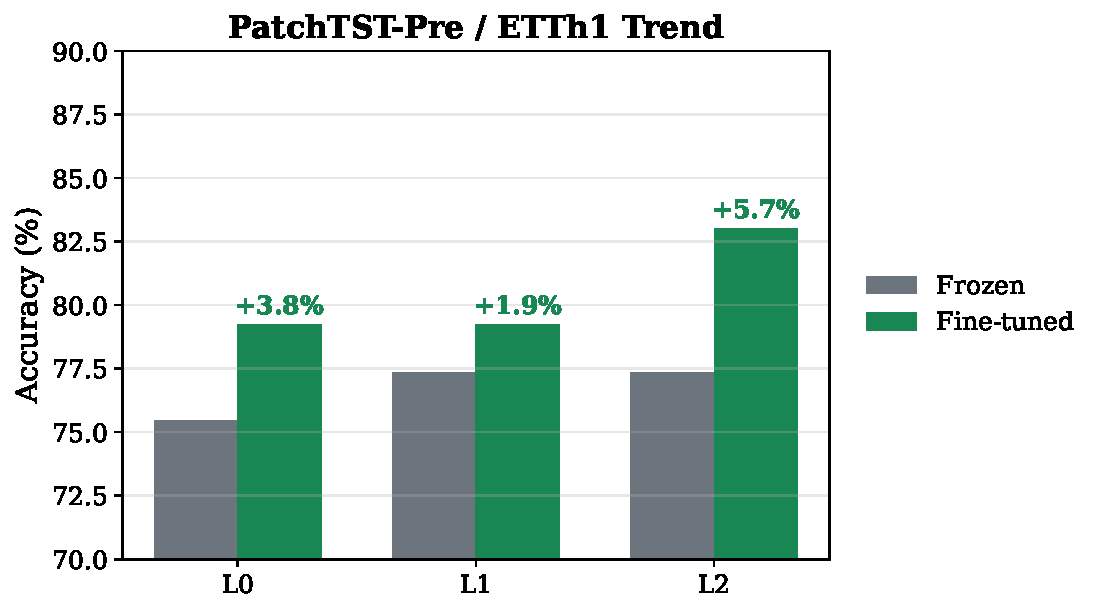
\includegraphics[width=0.6\textwidth]{figures/fig8_finetune.pdf}
    \caption{Trend detection accuracy after fine-tuning PatchTST-Pre on ETTh1. Gains are positive but concentrated in the best middle layer.}
    \label{fig:finetune_fig}
\end{figure}

\begin{figure}[tbp]
    \centering
    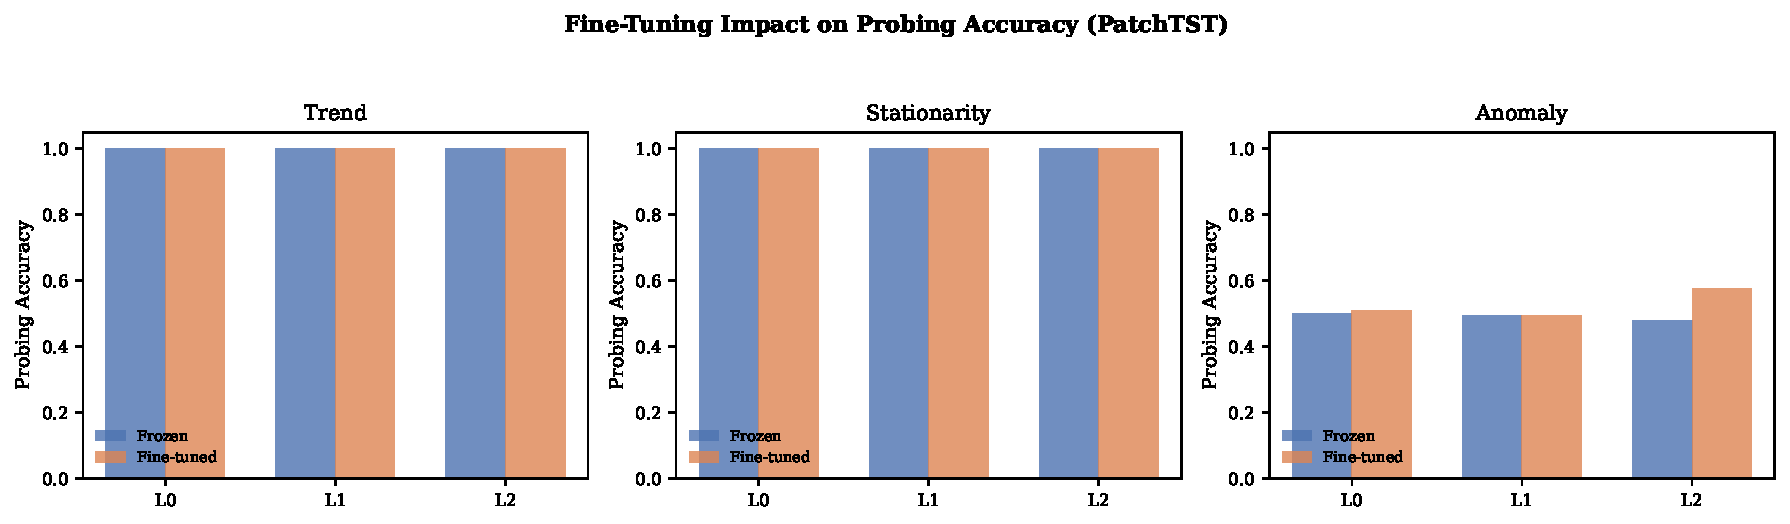
\includegraphics[width=\textwidth]{figures/fig24_finetuning_prediction.pdf}
    \caption{Frozen-vs-fine-tuned probe accuracy. Fine-tuning gains concentrate on anomaly, while trend and stationarity remain near ceiling.}
    \label{fig:finetuning_prediction}
\end{figure}

\subsection{Selectivity Analysis}

\Cref{tab:selectivity} reports selectivity ($\text{Acc}_{\text{linear}} - \text{Acc}_{\text{MLP}}$) for all models. Near-zero selectivity indicates that temporal information is trivially linearly accessible, while negative selectivity means the MLP control probe outperforms the linear probe.

\begin{table}[tbp]
\caption{Selectivity (Linear Accuracy $-$ MLP Control Accuracy) for all models.}
\label{tab:selectivity}
\centering
\resizebox{\textwidth}{!}{
\begin{tabular}{lcccccc}
\toprule
Model & Trend & Season.\ (R\textsuperscript{2}) & Frequency & Station.\ & Anomaly & Change Pt.\ \\
\midrule
MOMENT-PCA512 & +0.000 & -2.117 & +0.000 & +0.000 & +0.002 & +0.000 \\
Chronos-Bolt & +0.000 & -0.000 & +0.000 & +0.000 & -0.010 & +0.000 \\
PatchTST-Pre & +0.000 & -0.000 & +0.000 & +0.000 & +0.010 & +0.000 \\
GPT4TS-PCA512 & +0.000 & -2.040 & +0.000 & +0.000 & -0.006 & +0.000 \\
Timer-Base & +0.000 & --- & +0.000 & +0.000 & +0.000 & +0.000 \\
TimesFM-500M & +0.000 & -0.035 & +0.000 & +0.000 & -0.110 & +0.000 \\
Moirai-Small & +0.000 & -0.002 & +0.000 & +0.000 & -0.090 & +0.000 \\
\midrule
PatchTST-Rnd & +0.000 & -0.001 & +0.000 & -0.536 & -0.102 & -0.002 \\
iTransf.-Rnd & +0.000 & -0.001 & +0.000 & -0.002 & -0.020 & +0.000 \\
\bottomrule
\end{tabular}
}
\end{table}

\subsection{Cross-LEACE Asymmetry Analysis}

\Cref{tab:cross_leace_asymmetry} quantifies directional dependency between concept pairs by comparing accuracy drops in both directions. High asymmetry indicates that one concept's representation depends on the other, but not vice versa.

\begin{table}[tbp]
\caption{Cross-LEACE Asymmetry Analysis. Absolute difference in accuracy drop when erasing concept A to evaluate B vs.\ erasing B to evaluate A.}
\label{tab:cross_leace_asymmetry}
\centering
\begin{tabular}{llccc}
\toprule
Model & Concept Pair & Forward Drop & Reverse Drop & Asymmetry \\
\midrule
MOMENT & Change Pt.\ $\leftrightarrow$ Stationarity & 40.9\% & 40.7\% & 0.2\% \\
MOMENT & Change Pt.\ $\leftrightarrow$ Trend & 36.0\% & 0.0\% & 36.0\% \\
MOMENT & Stationarity $\leftrightarrow$ Trend & 3.3\% & 12.2\% & 8.9\% \\
\midrule
GPT4TS & Change Pt.\ $\leftrightarrow$ Stationarity & 26.2\% & 47.7\% & 21.5\% \\
GPT4TS & Change Pt.\ $\leftrightarrow$ Trend & 34.0\% & 38.0\% & 4.0\% \\
GPT4TS & Stationarity $\leftrightarrow$ Trend & 0.0\% & 17.6\% & 17.6\% \\
\bottomrule
\end{tabular}
\end{table}

\subsection{Sample Efficiency of Linear Probes}

We train linear probes on the best layer with varying training set sizes (100--5000 samples). For \textbf{trend detection}, Chronos-Bolt, PatchTST-Pre, and GPT4TS achieve 100\% accuracy with as few as 100 samples, indicating that trend information is linearly accessible with minimal supervision under this synthetic setup. MOMENT-PCA512 requires $\sim$500 samples to stabilize at 97\%, consistent with the PCA-reduced probe setup requiring more data to converge. For \textbf{stationarity}, Chronos-Bolt achieves 100\% from 100 samples, while PatchTST-Pre and GPT4TS start at 93\% and converge by 500 samples. MOMENT-PCA512 shows the slowest convergence, requiring $\sim$2500 samples to reach near-perfect accuracy. This gap reinforces the PCA bottleneck finding: dimensionality reduction forces the linear probe to compensate with more training data.

\begin{figure}[tbp]
    \centering
    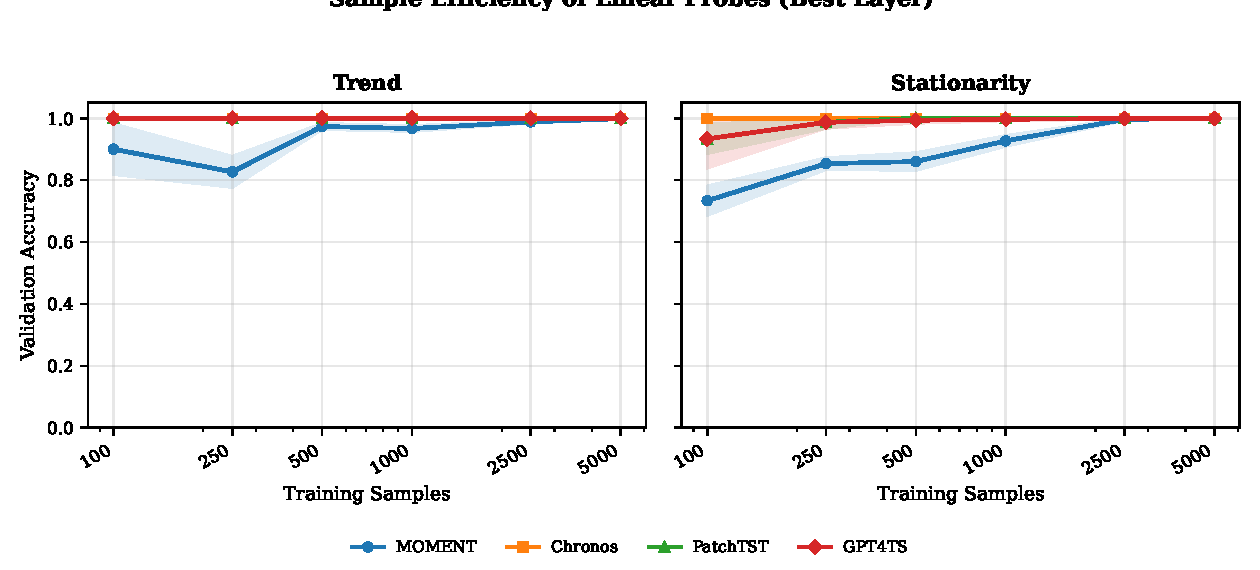
\includegraphics[width=0.85\textwidth]{figures/fig10_sample_efficiency.pdf}
    \caption{Sample efficiency of linear probes at the best layer. Trend and stationarity saturate with surprisingly little supervision in most families.}
    \label{fig:sample_efficiency}
\end{figure}

\subsection{Real-World LEACE Erasure}

\Cref{tab:realworld_leace} shows LEACE concept erasure applied to real-world datasets (ETTh1, Weather) for trend and stationarity. Unlike synthetic data where trend drops are often modest, real-world \textbf{Weather trend} shows large degradations: Chronos-Bolt loses 48.0\% accuracy, GPT4TS 42.9\%, and PatchTST-Pre 40.5\%, while MOMENT shows an 18.0\% drop. This indicates that real-world trend representations can also be sensitive to linear erasure of trend subspaces. On ETTh1, trend erasure effects are smaller: GPT4TS drops 15.1\%, Chronos 9.4\%, PatchTST 7.5\%, and MOMENT only 3.8\%.

\textbf{Stationarity} erasure shows varied sensitivity: MOMENT drops 20.8\% on ETTh1 and GPT4TS 15.1\%, while Chronos-Bolt is nearly unaffected (1.9\%). On Weather, stationarity erasure has minimal impact for Chronos, PatchTST, and GPT4TS ($\leq$3.5\%) but remains substantial for MOMENT (16.5\%), indicating that stationarity is encoded more diffusely in some families than in others.

\begin{table}[tbp]
\caption{Real-world LEACE erasure: best-layer accuracy before/after erasure and accuracy drop.}
\label{tab:realworld_leace}
\centering
\resizebox{\textwidth}{!}{
\begin{tabular}{llcccccccc}
\toprule
& & \multicolumn{4}{c}{ETTh1} & \multicolumn{4}{c}{Weather} \\
\cmidrule(lr){3-6} \cmidrule(lr){7-10}
Model & Property & Before & After & Drop & Layer & Before & After & Drop & Layer \\
\midrule
MOMENT & Trend & 96.2 & 92.5 & 3.8 & L10 & 99.0 & 81.0 & 18.0 & L6 \\
MOMENT & Station. & 96.2 & 75.5 & 20.8 & L12 & 88.5 & 72.0 & 16.5 & L6 \\
Chronos & Trend & 96.2 & 86.8 & 9.4 & L0 & 99.5 & 51.5 & 48.0 & L0 \\
Chronos & Station. & 100.0 & 98.1 & 1.9 & L0 & 98.5 & 95.0 & 3.5 & L5 \\
PatchTST & Trend & 98.1 & 90.6 & 7.5 & L1 & 100.0 & 59.5 & 40.5 & L2 \\
PatchTST & Station. & 100.0 & 94.3 & 5.7 & L2 & 93.5 & 93.0 & 0.5 & L2 \\
GPT4TS & Trend & 98.1 & 83.0 & 15.1 & L11 & 98.5 & 55.6 & 42.9 & L6 \\
GPT4TS & Station. & 94.3 & 79.2 & 15.1 & L2 & 90.3 & 86.9 & 3.3 & L1 \\
\bottomrule
\end{tabular}
}
\end{table}

\subsection{PCA Dimension Sweep}

\Cref{fig:pca_sweep} shows the complete PCA dimension sweep for seasonality regression. Across all tested dimensions (64--512), PCA-reduced representations yield negative R\textsuperscript{2}, suggesting that top-variance principal components are poorly aligned with the seasonality-relevant subspace in this probe setup. The monotonically worsening R\textsuperscript{2} with more components further suggests that additional PCA dimensions introduce variance-capturing directions that interfere with seasonality prediction.

\begin{figure}[tbp]
    \centering
    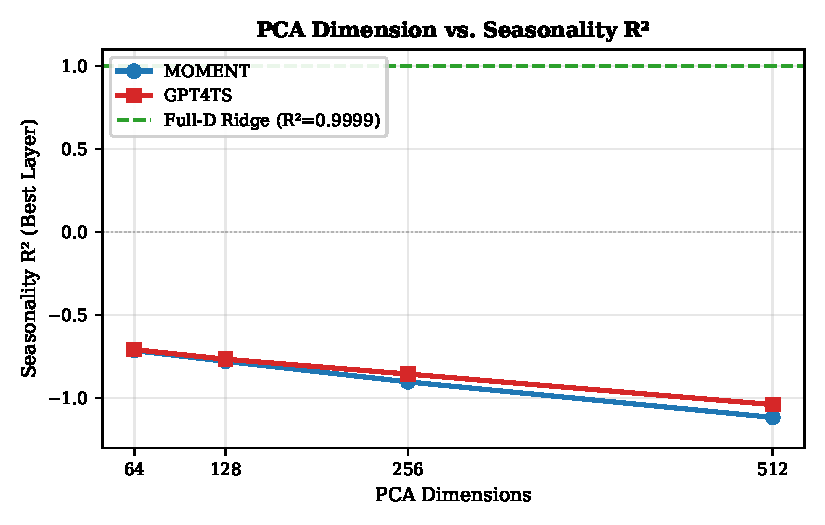
\includegraphics[width=0.65\textwidth]{figures/fig11_pca_sweep_seasonality.pdf}
    \caption{PCA dimension sweep for seasonality R\textsuperscript{2}. All PCA dimensions remain negative, whereas full-dimensional Ridge recovers near-perfect performance.}
    \label{fig:pca_sweep}
\end{figure}

\subsection{t-SNE Representation Visualizations}

\Cref{fig:tsne_trend,fig:tsne_stationarity} show t-SNE projections of Layer 0 and best layer representations for trend and stationarity classification. Chronos-Bolt and PatchTST-Pre show clear class separation from Layer 0, consistent with their high probing accuracy. GPT4TS shows less distinct boundaries, reflecting its PCA-compressed representation. MOMENT-PCA512 shows moderate separation that improves in later layers for trend.

\begin{figure}[tbp]
    \centering
    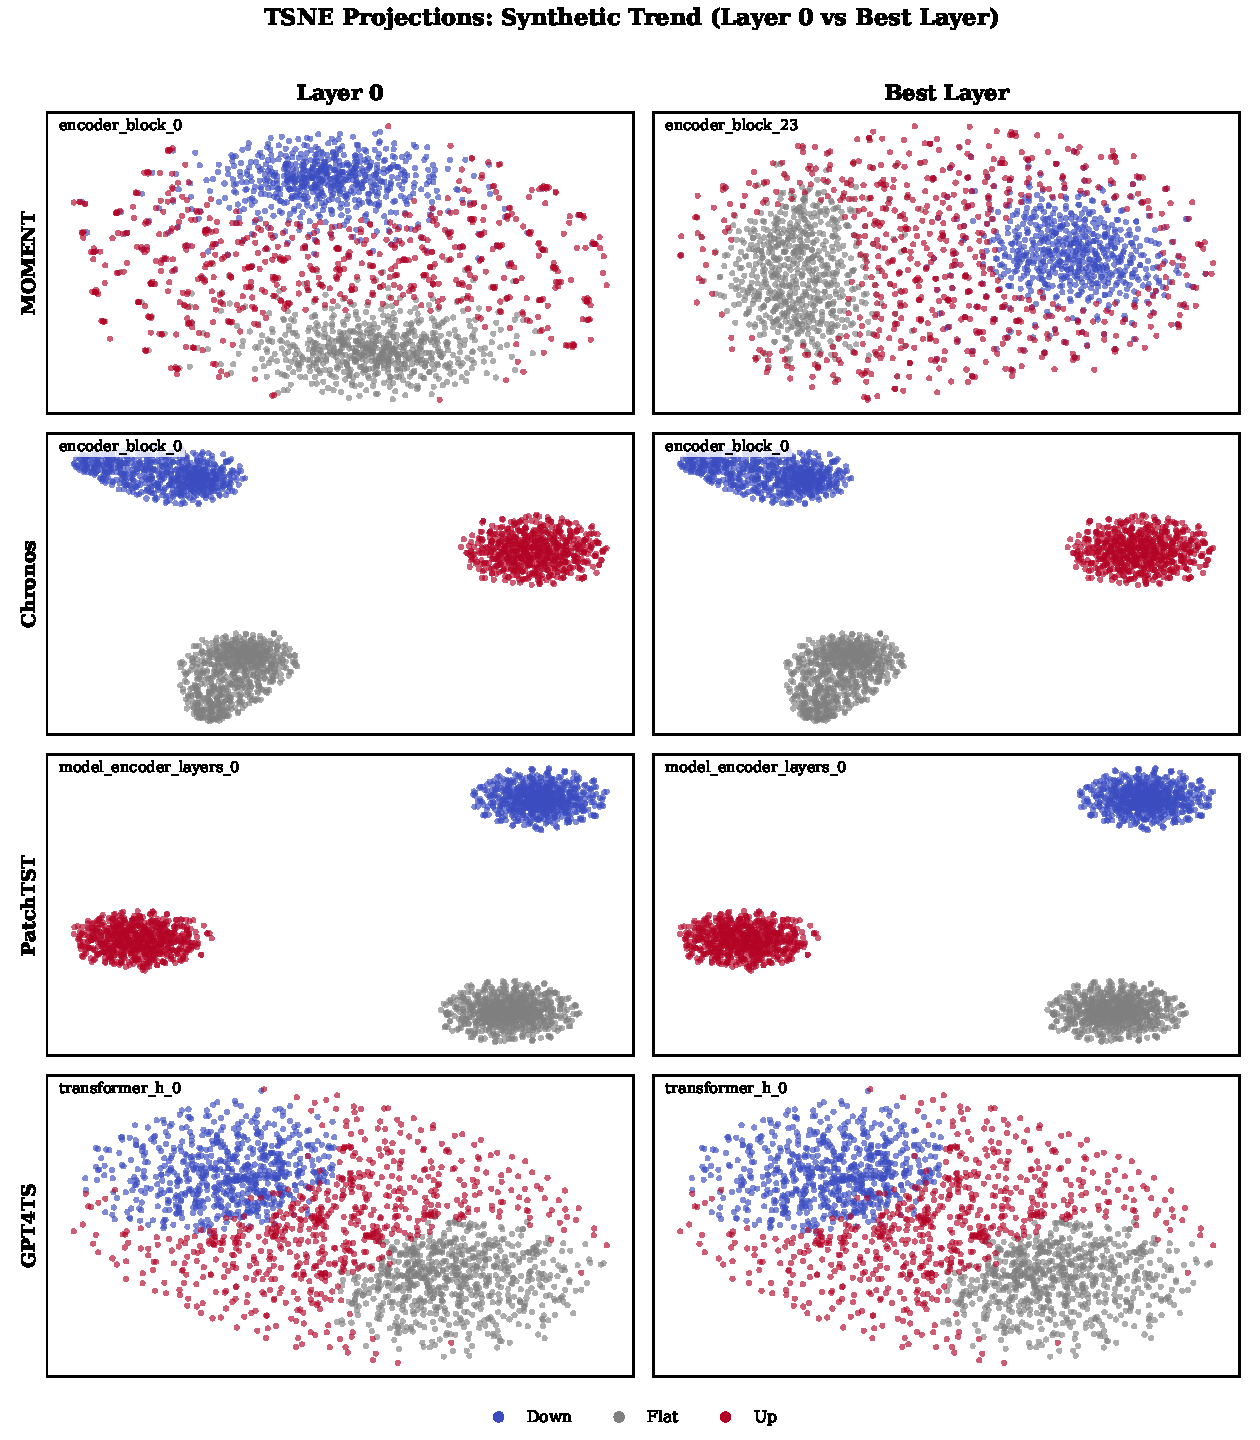
\includegraphics[width=0.90\textwidth]{figures/fig12_tsne_trend.pdf}
    \caption{t-SNE projections for synthetic trend at Layer 0 versus the best layer. Separation is already visible early for the clearest-performing families.}
    \label{fig:tsne_trend}
\end{figure}

\begin{figure}[tbp]
    \centering
    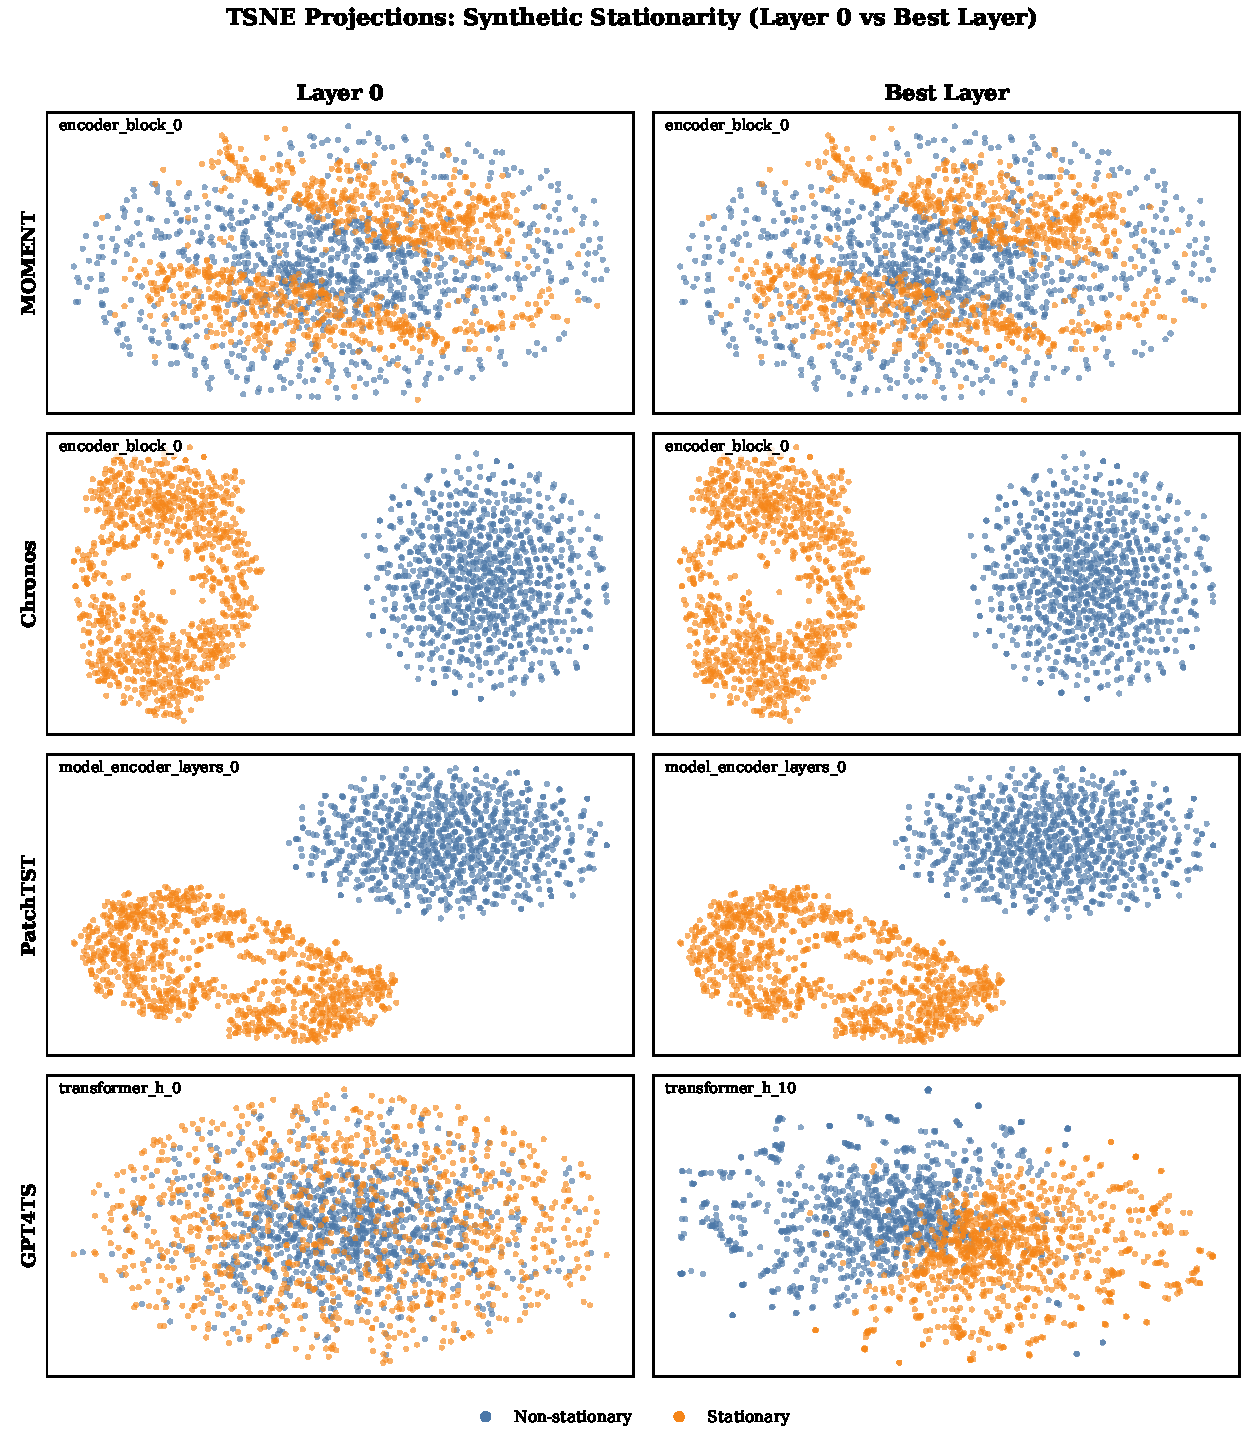
\includegraphics[width=0.80\textwidth]{figures/fig13_tsne_stationarity.pdf}
    \caption{t-SNE projections for synthetic stationarity at Layer 0 versus the best layer. Class separation sharpens only modestly with depth.}
    \label{fig:tsne_stationarity}
\end{figure}

\subsection{UMAP Representation Visualizations}

\Cref{fig:umap_trend,fig:umap_stationarity} complement the t-SNE projections with UMAP, which better preserves global structure. The results are qualitatively consistent: Chronos-Bolt and PatchTST-Pre show clear class separation from Layer~0, while GPT4TS-PCA512 shows diffuse boundaries.

\begin{figure}[tbp]
    \centering
    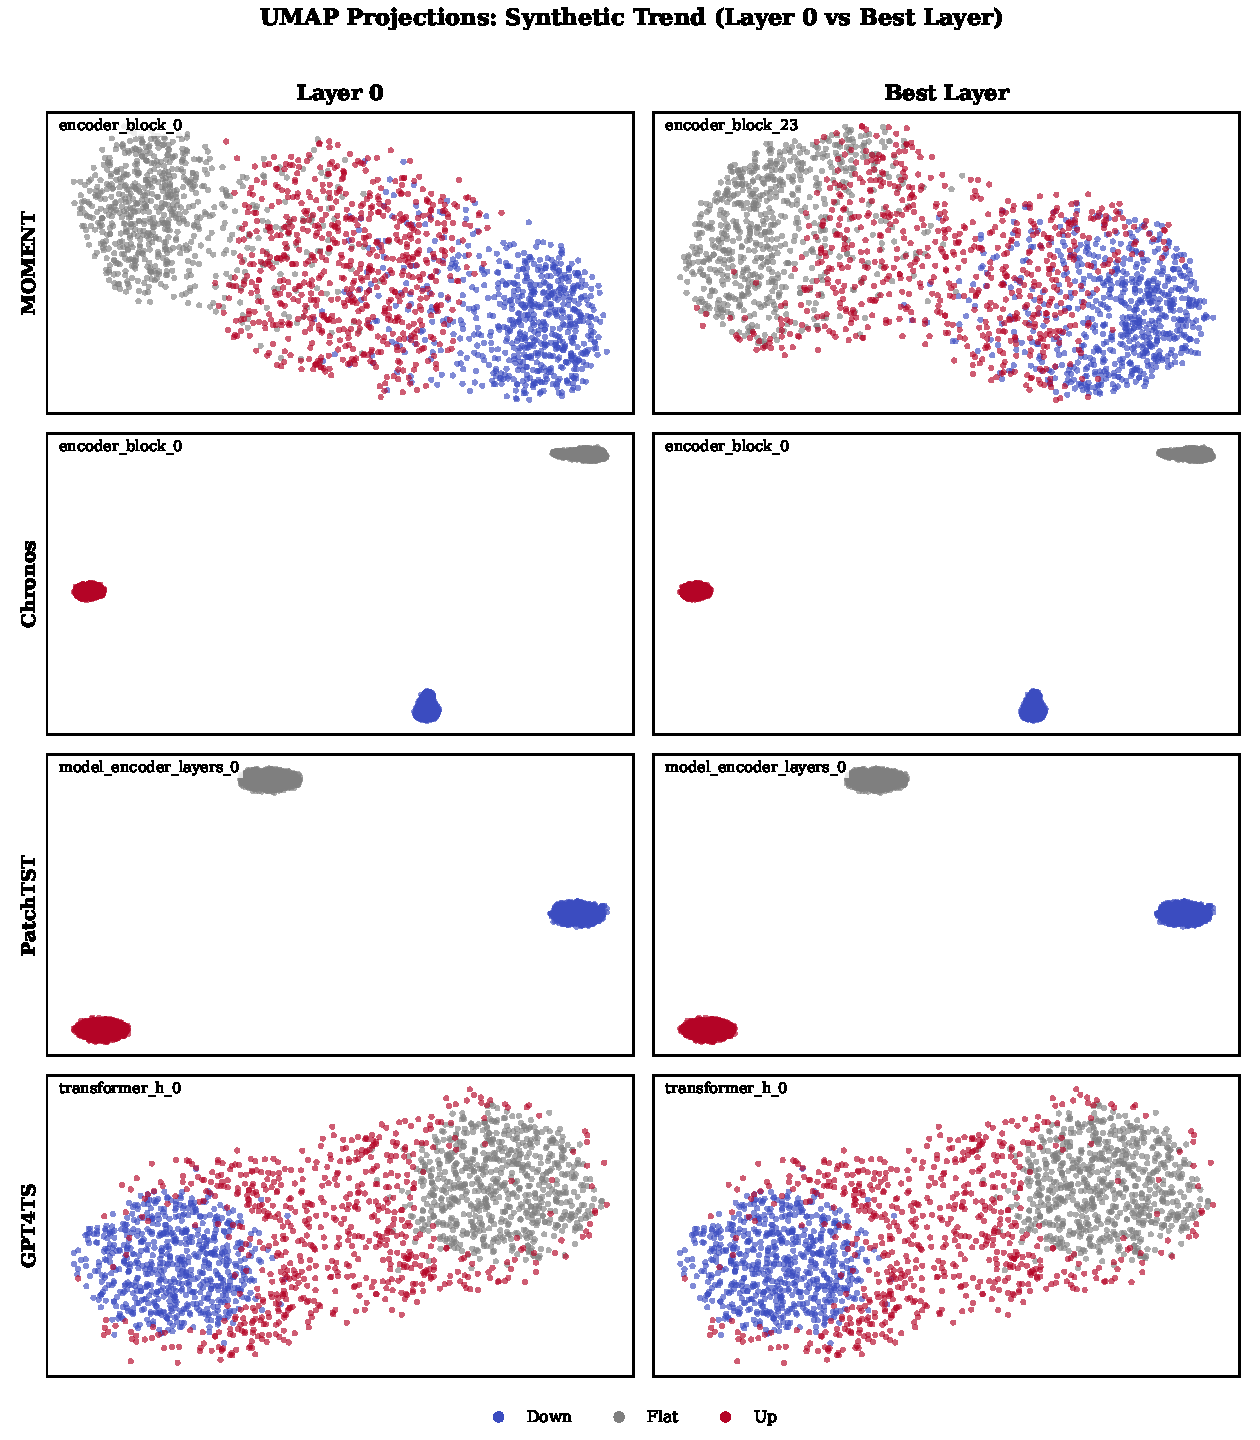
\includegraphics[width=0.80\textwidth]{figures/fig14_umap_trend.pdf}
    \caption{UMAP projections for synthetic trend at Layer 0 versus the best layer. Global structure mirrors the t-SNE trends.}
    \label{fig:umap_trend}
\end{figure}

\begin{figure}[tbp]
    \centering
    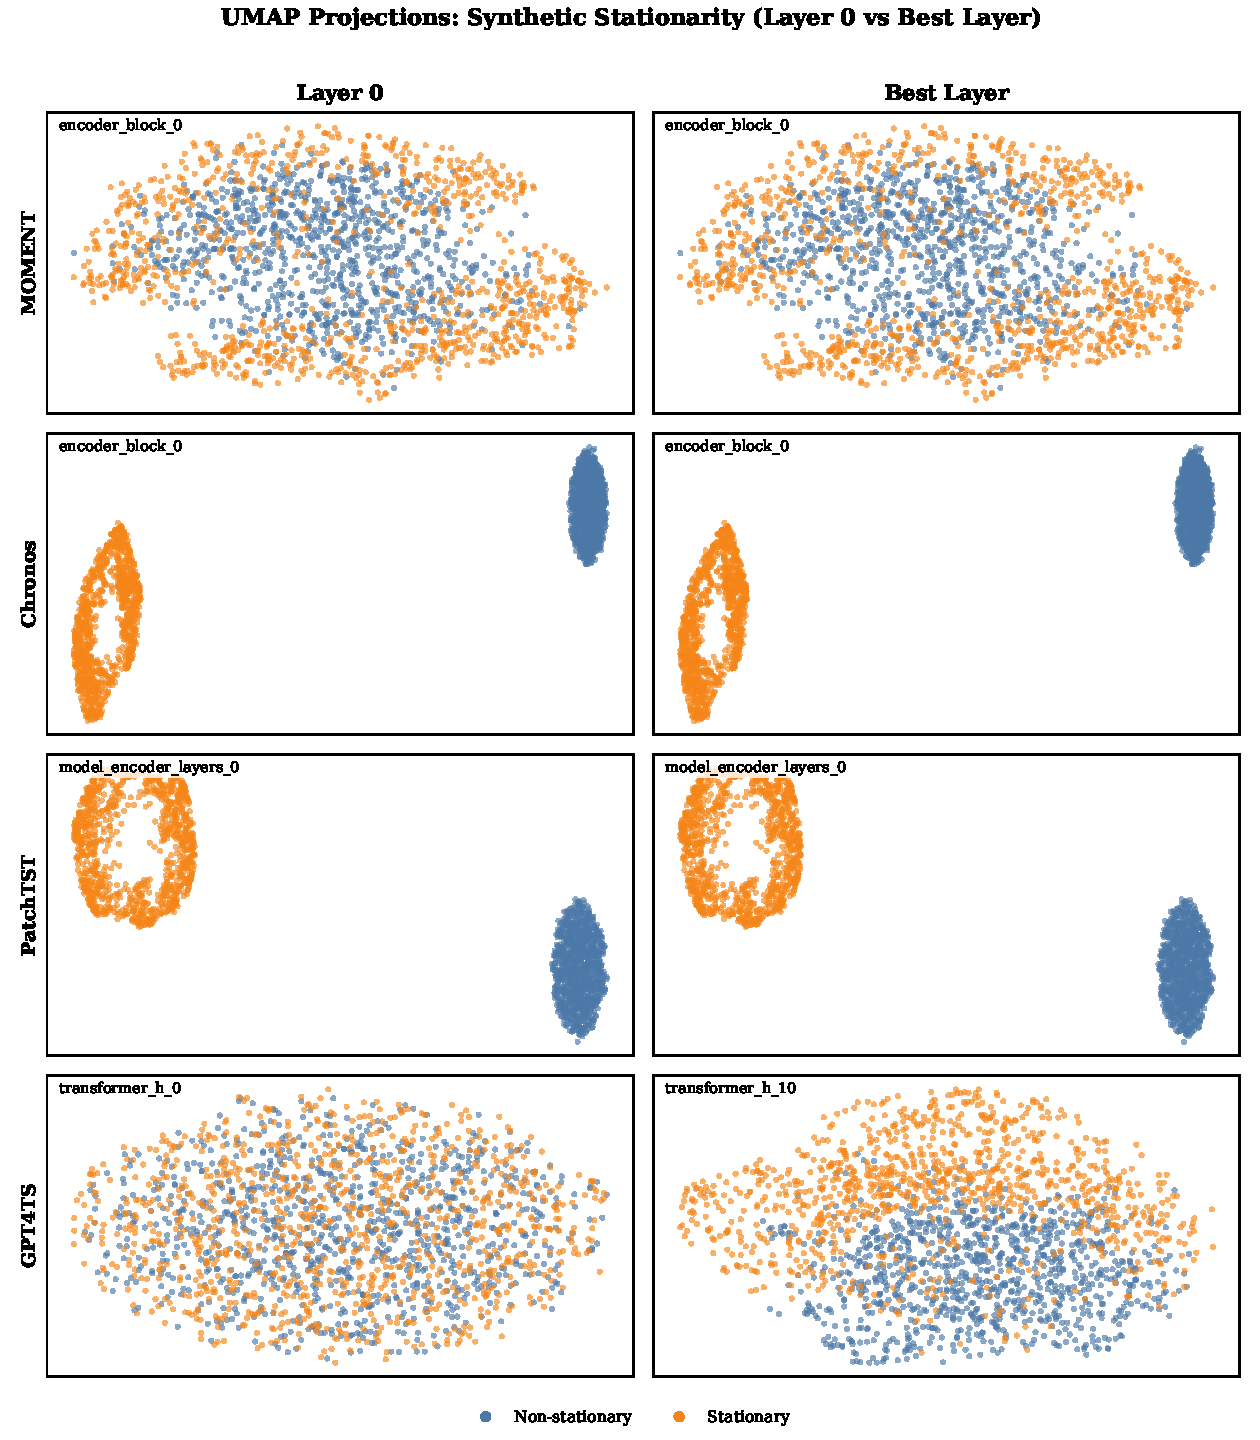
\includegraphics[width=0.90\textwidth]{figures/fig15_umap_stationarity.pdf}
    \caption{UMAP projections for synthetic stationarity at Layer 0 versus the best layer. Global structure remains more diffuse than for trend.}
    \label{fig:umap_stationarity}
\end{figure}

\subsection{PatchTST Attention Pattern Analysis}

\Cref{fig:attention_analysis} shows attention entropy and mean attention distance across PatchTST-Pre's 3 layers for trend and seasonality. For \textbf{trend}, attention entropy dips in Layer~1 (3.43 vs.\ 3.67 in L0), suggesting the middle layer specializes with sharper attention patterns. Per-class analysis reveals the \textit{Up} class consistently receives higher entropy (more diffuse attention) than \textit{Down}, potentially reflecting asymmetric pattern complexity. Mean attention distance also decreases in Layer~1, indicating more localized processing. For \textbf{seasonality}, entropy and distance follow similar layer-wise patterns but without per-class differentiation (binary property).

\begin{figure}[tbp]
    \centering
    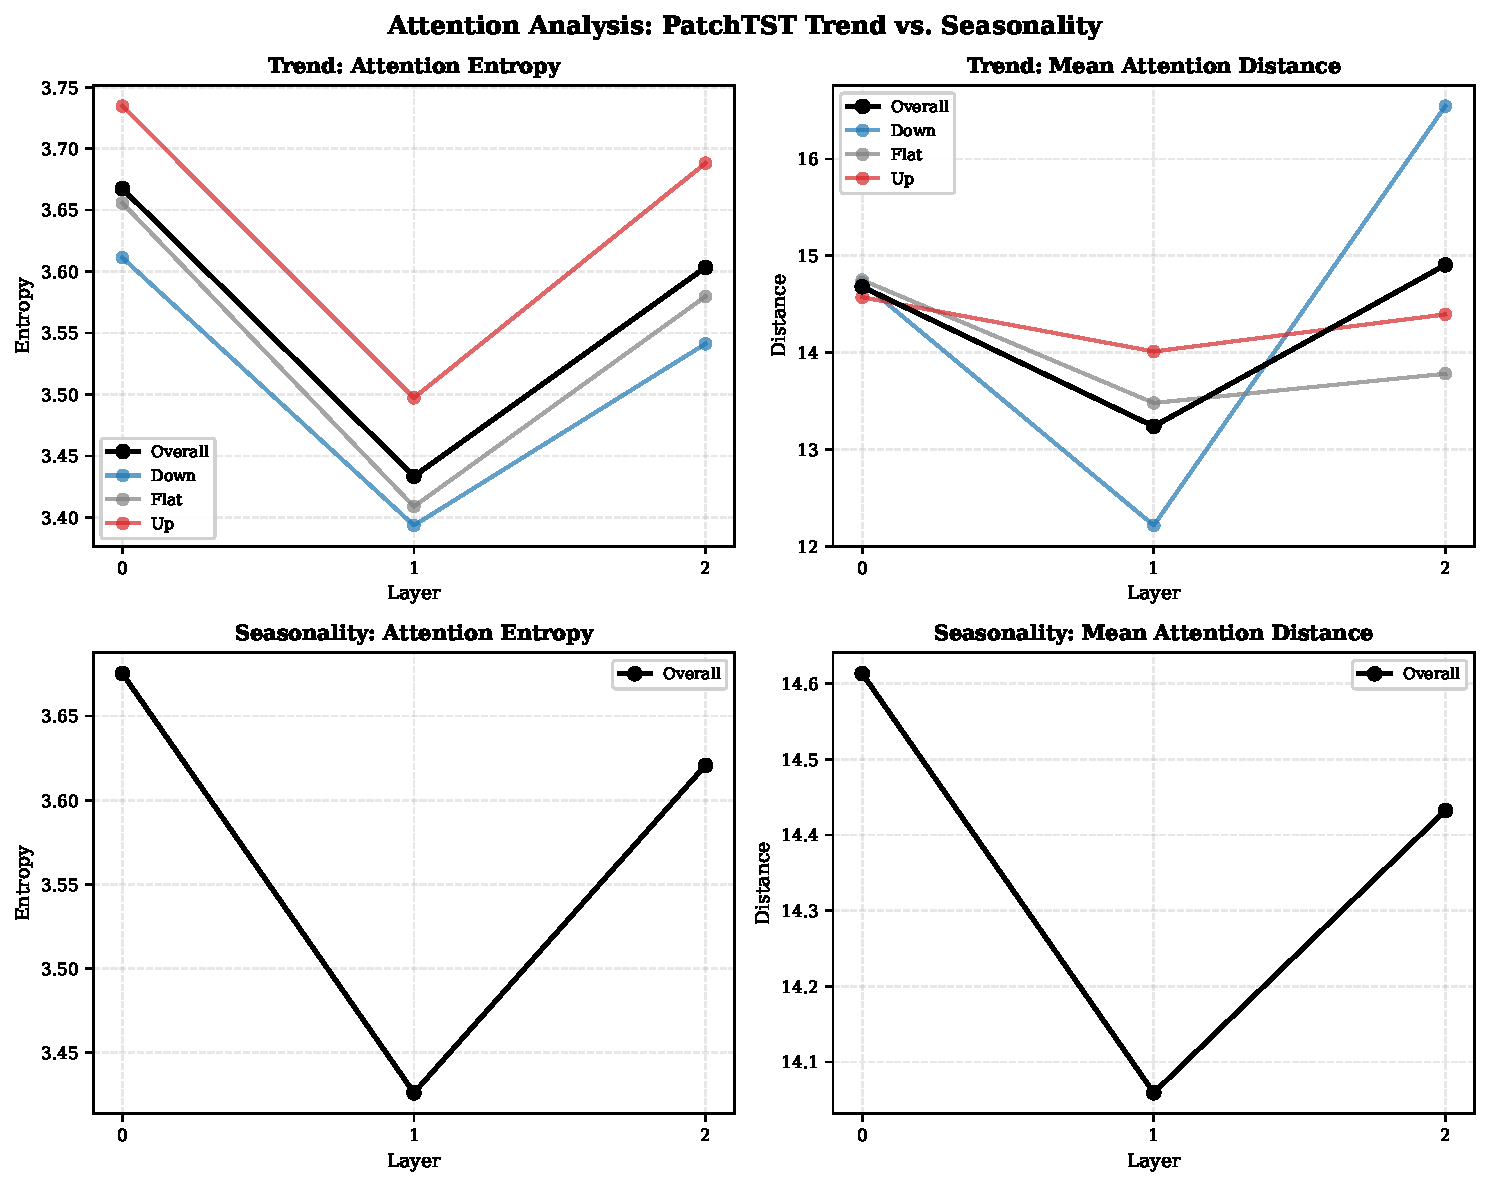
\includegraphics[width=0.85\textwidth]{figures/fig16_attention_analysis.pdf}
    \caption{PatchTST attention entropy and mean distance across layers. The middle layer shows the sharpest, most localized attention patterns.}
    \label{fig:attention_analysis}
\end{figure}

\subsection{Anomaly Noise Robustness}

\Cref{fig:anomaly_noise} shows probe accuracy as anomaly magnitude (signal-to-noise ratio) varies from 1.0 to 8.0. \textbf{Chronos-Bolt} shows the largest observed robustness gain, scaling from 48.6\% at magnitude~1.0 (near-random) to 88.6\% at magnitude~8.0. MOMENT follows at 70.8\%, while PatchTST-Pre (54.4\%) and GPT4TS (54.3\%) remain near random even at high SNR. In this setup, decoder-style models appear to encode anomaly signal strength more accessibly than patch-based models.

\begin{figure}[tbp]
    \centering
    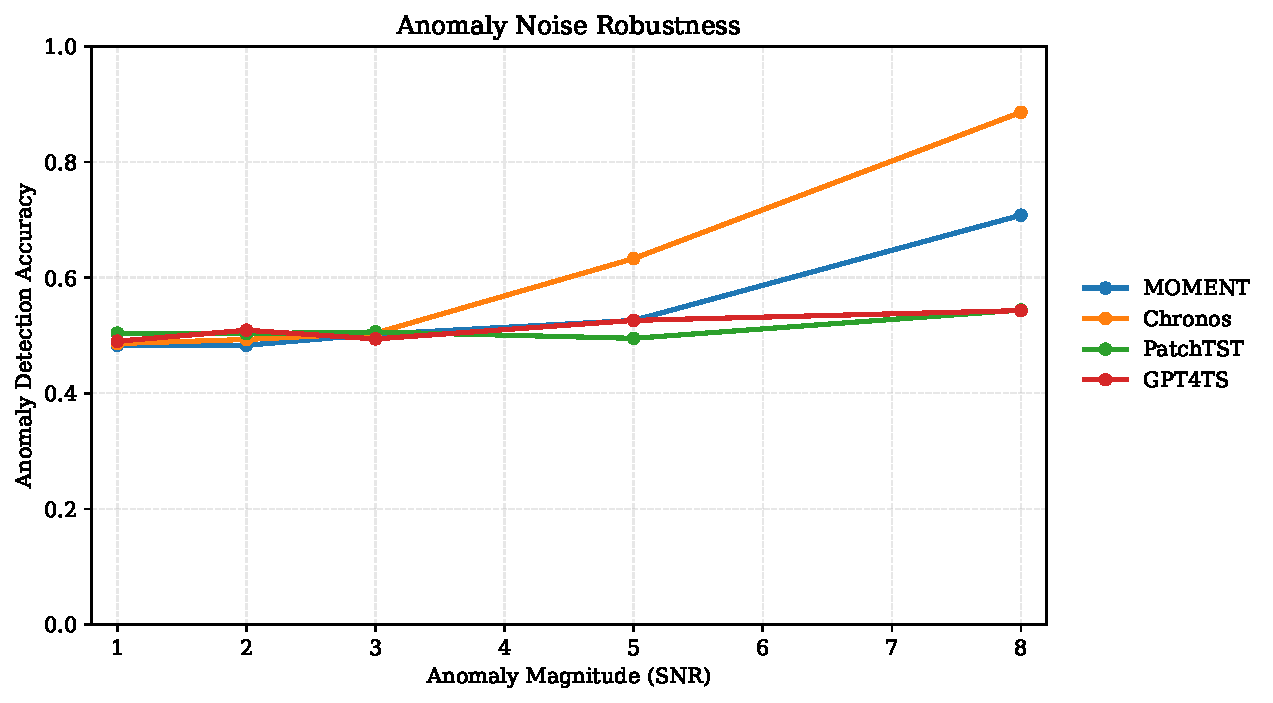
\includegraphics[width=0.65\textwidth]{figures/fig17_anomaly_noise.pdf}
    \caption{Anomaly detection accuracy versus anomaly magnitude (SNR) across model families. Decoder-style models benefit most from stronger anomaly signal.}
    \label{fig:anomaly_noise}
\end{figure}

\subsection{Downstream Reconstruction Impact of Concept Erasure}

\Cref{fig:downstream_impact} quantifies how LEACE erasure affects MOMENT's downstream reconstruction quality. For \textbf{trend} erasure, early layers show minimal impact (L0: +1.0\% MSE), middle layers show the most degradation (L11: +5.6\%), and the final layer shows an unexpected MSE \emph{decrease} ($-$17.2\%). This suggests that trend information in late layers may be redundant or interfere with reconstruction, and erasing it may act as a form of regularization. For \textbf{stationarity}, the pattern is similar: early erasure has modest impact (L0: +5.8\%), while middle-layer erasure causes the largest degradation (L11: +18.0\%). This places the largest observed stationarity sensitivity in middle encoder blocks.

\begin{figure}[tbp]
    \centering
    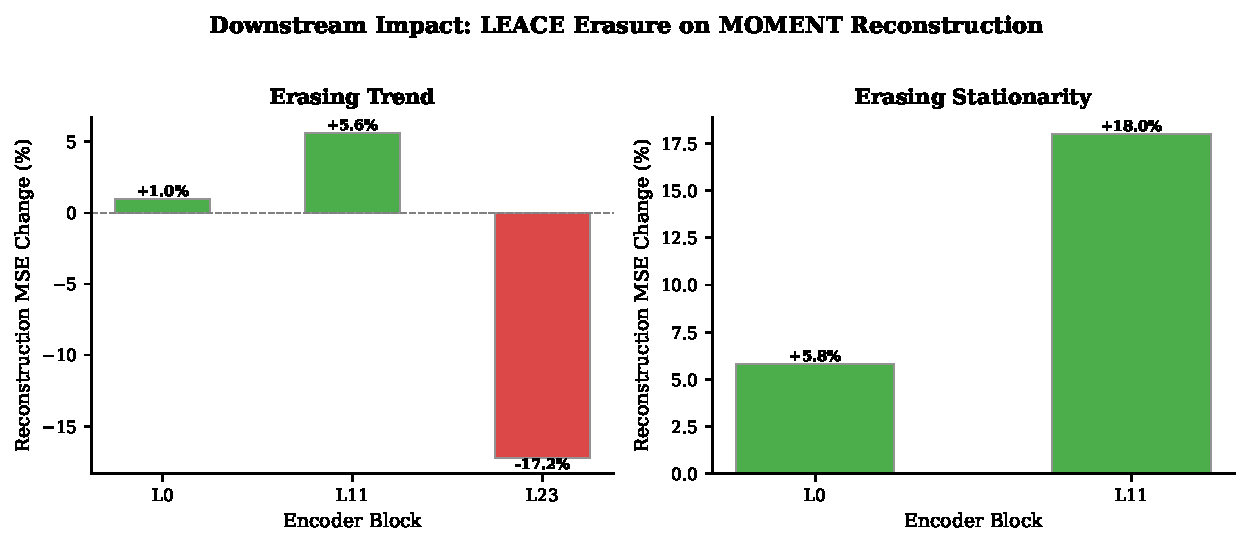
\includegraphics[width=0.75\textwidth]{figures/fig18_downstream_impact.pdf}
    \caption{Reconstruction MSE change (\%) after LEACE erasure at MOMENT layers. Middle-layer erasure produces the largest downstream degradation in this analysis.}
    \label{fig:downstream_impact}
\end{figure}

\subsection{Downstream Forecasting Impact (Chronos-Bolt)}

\Cref{fig:chronos_downstream} extends the interventional analysis to Chronos-Bolt's forecasting task (64-step horizon). \textbf{Trend} erasure causes very large degradation, especially at early layers: L0 produces +7808\% MSE increase, L2 +644\%, and L5 +1571\%. This is much larger than MOMENT's trend erasure effects, indicating that Chronos-Bolt's forecasting relies heavily on early-layer trend encoding. \textbf{Stationarity} erasure has negligible impact ($-$1.0\% at L0, +8.7\% at L2, $-$2.1\% at L5), suggesting stationarity information is either redundant for forecasting or encoded non-linearly.

\begin{figure}[tbp]
    \centering
    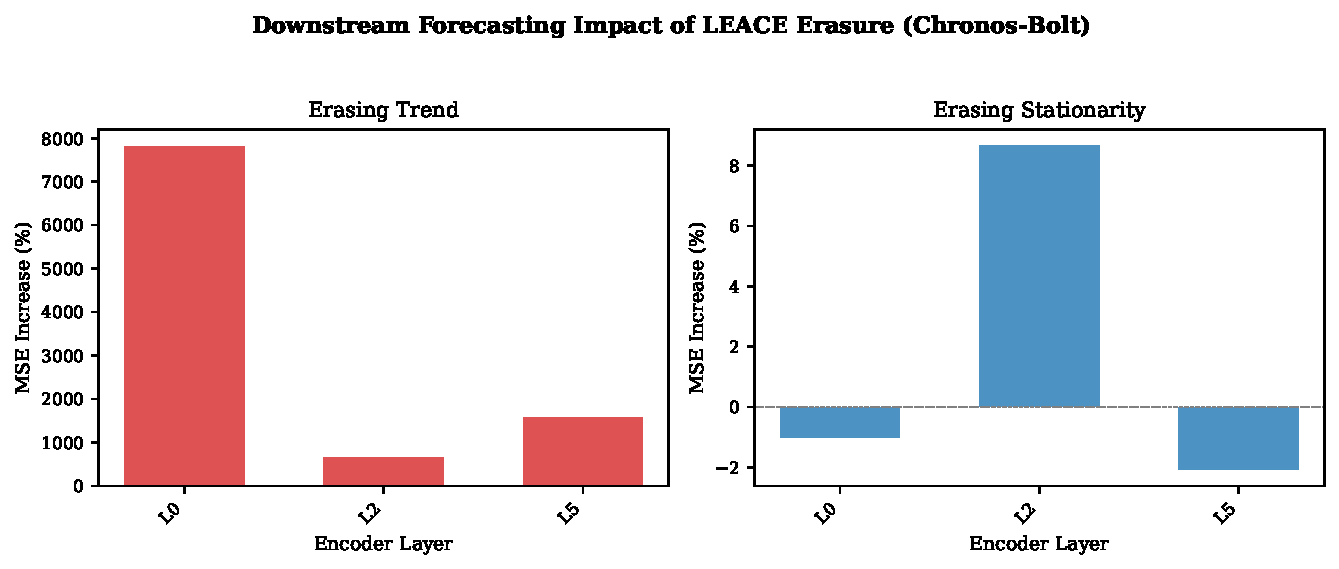
\includegraphics[width=0.75\textwidth]{figures/fig19_chronos_downstream_impact.pdf}
    \caption{Forecasting MSE change (\%) after LEACE erasure at Chronos-Bolt layers. Early trend erasure has the largest downstream effect.}
    \label{fig:chronos_downstream}
\end{figure}

\subsection{Downstream Output Impact (GPT4TS)}

\Cref{fig:gpt4ts_downstream} measures the output divergence of GPT4TS (frozen GPT-2) after LEACE erasure, complementing the reconstruction (MOMENT) and forecasting (Chronos-Bolt) analyses. Unlike native TSFMs, GPT4TS exhibits a distinct pattern: \textbf{stationarity} erasure causes the largest output disruption (55.1\% divergence at L5), substantially exceeding trend erasure (37.5\% at L5). This asymmetry is reversed compared to Chronos-Bolt, where trend erasure dominates. Notably, late-layer (L11) erasure has the least impact for both properties (4.2\% trend, 24.4\% stationarity), suggesting the frozen LLM backbone consolidates temporal concepts in middle layers. This mid-layer concentration mirrors MOMENT's reconstruction pattern but contrasts with Chronos-Bolt's early-layer reliance, revealing architecture-specific intervention pathways.

\begin{figure}[tbp]
    \centering
    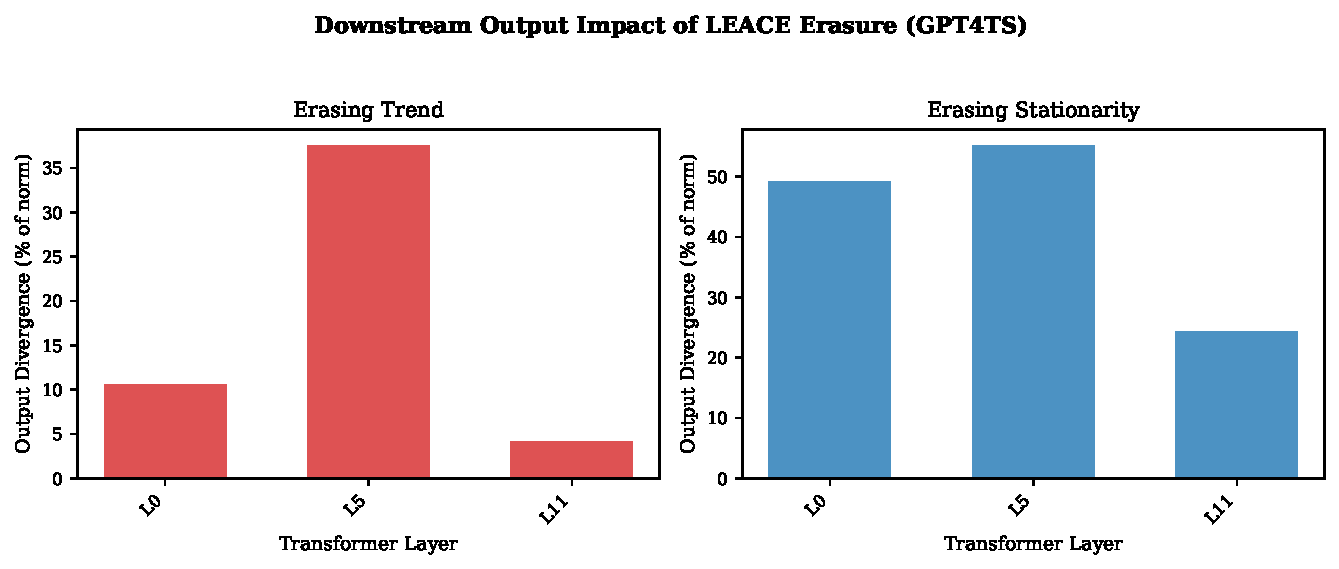
\includegraphics[width=0.75\textwidth]{figures/fig20_gpt4ts_downstream_impact.pdf}
    \caption{Output divergence (\% of output norm) after LEACE erasure at GPT4TS layers. Stationarity removal perturbs outputs more than trend removal.}
    \label{fig:gpt4ts_downstream}
\end{figure}

\subsection{Downstream Forecasting Impact (TimesFM)}

\Cref{fig:timesfm_downstream} extends interventional analysis to TimesFM, the largest decoder-only model (494M, 50 layers). \textbf{Trend} erasure produces the most extreme relative effects in our study: even early-layer erasure (L0) increases forecast MSE by +195,775\%, escalating to +413,099\% at L49. Because these are relative MSE changes, they should be interpreted as instability indicators rather than directly comparable effect sizes across models. \textbf{Stationarity} erasure, by contrast, has negligible impact ($-$1.6\% to +5.0\%), mirroring Chronos-Bolt's pattern and suggesting that, in this setup, decoder-only forecasting is much more sensitive to trend-subspace removal than to stationarity-subspace removal.

\begin{figure}[tbp]
    \centering
    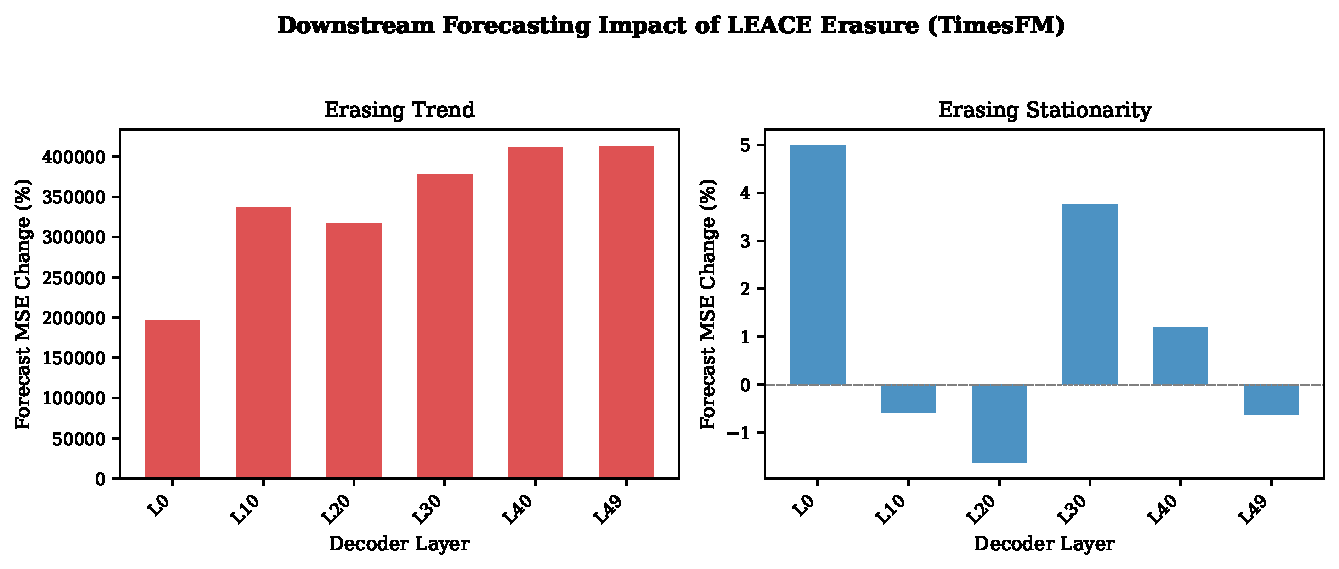
\includegraphics[width=0.75\textwidth]{figures/fig21_timesfm_downstream_impact.pdf}
    \caption{Forecasting MSE change (\%) after LEACE erasure at TimesFM decoder layers. Trend erasure causes very large degradation at all layers.}
    \label{fig:timesfm_downstream}
\end{figure}

\subsection{Downstream Output Impact (Moirai v2)}

\Cref{fig:moirai_downstream} measures Moirai v2's output divergence after LEACE erasure. Unlike decoder-only models, Moirai shows a \textbf{reversed priority}: \textbf{stationarity} erasure causes larger output disruption (peak 10.9\% divergence at L1) than \textbf{trend} erasure (peak 3.2\% at L0). Both properties show a decreasing impact with depth (L0 most affected, L5 least), consistent with Moirai's compact encoder architecture concentrating intervention-sensitive information in early layers. The overall magnitudes are modest compared to TimesFM's large trend sensitivity, reflecting Moirai's smaller parameter count (11.4M vs.\ 494M) and shallower error amplification chain.

\begin{figure}[tbp]
    \centering
    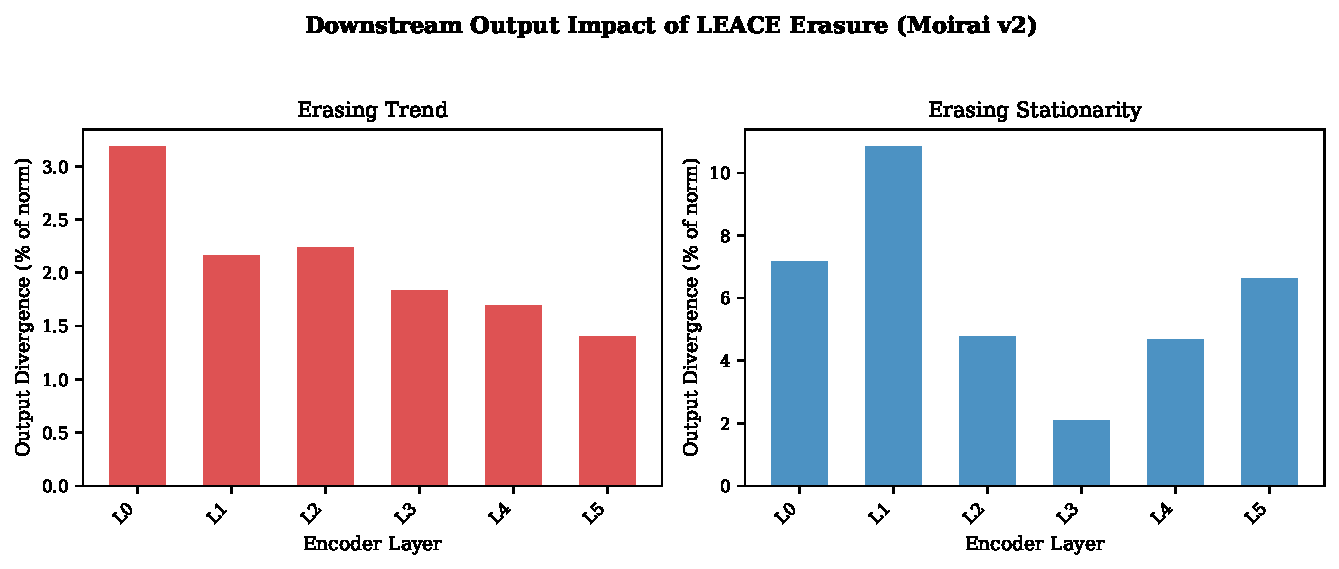
\includegraphics[width=0.75\textwidth]{figures/fig22_moirai_downstream_impact.pdf}
    \caption{Output divergence (\% of output norm) after LEACE erasure at Moirai layers. Stationarity has the stronger downstream footprint.}
    \label{fig:moirai_downstream}
\end{figure}

\subsection{Timer Model Probing Results}

Timer \cite{Liu2024b}, a decoder-only generative TSFM with 84M parameters and 8 layers, shows
probing performance consistent with other pre-trained models. \textbf{Trend}, \textbf{frequency},
\textbf{stationarity}, and \textbf{change point} are perfectly linearly separable from every
layer (100\% accuracy). \textbf{Seasonality} regression reaches R\textsuperscript{2}~=~0.998 at
Layer~5. However, \textbf{anomaly detection} remains weak (best 47.7\% averaged over 3 seeds at Layer~5), among the lowest of pre-trained models, indicating that point anomalies are challenging across architectural families.

\begin{table}[tbp]
\caption{Timer (84M) probing results: best-layer accuracy/R\textsuperscript{2} for each property.}
\label{tab:timer_probing}
\centering
\begin{tabular}{lcccccc}
\toprule
Model & Trend & Season.\ (R\textsuperscript{2}) & Frequency & Station.\ & Anomaly & Change Pt.\ \\
\midrule
Timer-Base & 1.000 & 0.998 & 1.000 & 1.000 & 0.460 & 1.000 \\
\bottomrule
\end{tabular}
\end{table}

\subsubsection{Timer LEACE Erasure}

LEACE erasure on Timer-Base (mean-pooled representations, $d$=1024) reveals decoder-specific erasure patterns:

\begin{table}[tbp]
\caption{Timer-Base LEACE erasure: accuracy/R\textsuperscript{2} before and after erasure at the
max-drop layer.}
\label{tab:timer_leace}
\centering
\small
\begin{tabular}{lcccl}
\toprule
Property & Before & After & Drop & Layer \\
\midrule
Trend & 1.000 & 0.665 & 0.335 & L0 \\
Seasonality (R\textsuperscript{2}) & 0.800 & $-$0.193 & 0.993 & L5 \\
Frequency & 1.000 & 0.800 & 0.200 & L0 \\
Stationarity & 0.995 & 0.365 & 0.630 & L0 \\
Anomaly & 0.680 & 0.640 & 0.040 & L3 \\
Change Point & 1.000 & 0.365 & 0.635 & L7 \\
\bottomrule
\end{tabular}
\end{table}

Timer concentrates trend, frequency, and stationarity erasure at \textbf{L0}, while change-point
vulnerability peaks at \textbf{L7}. This early-layer concentration mirrors Chronos-Bolt's
pattern, consistent with decoder-only architectures encoding structural properties immediately.
Seasonality is most vulnerable at L5 (R\textsuperscript{2} drops to $-$0.193), while anomaly
remains resistant to erasure (4\% drop), suggesting it is not linearly encoded in any single
direction.

\subsection{TimesFM and Moirai Probing Results}

TimesFM (494M, 50 decoder layers) and Moirai (11.4M, 6 encoder layers) extend our analysis to the largest and smallest models in the study.

\begin{table}[tbp]
\caption{TimesFM LEACE erasure: accuracy/R\textsuperscript{2} before and after erasure at the
max-drop layer (reported every 5th layer).}
\label{tab:timesfm_leace}
\centering
\small
\begin{tabular}{lcccl}
\toprule
Property & Before & After & Drop & Layer \\
\midrule
Trend & 1.000 & 0.630 & 0.370 & L5 \\
Seasonality (R\textsuperscript{2}) & 0.956 & $-$0.029 & 0.985 & L25 \\
Frequency & 1.000 & 0.635 & 0.365 & L0 \\
Stationarity & 1.000 & 0.300 & 0.700 & L0 \\
Anomaly & 0.800 & 0.645 & 0.155 & L25 \\
Change Point & 1.000 & 0.470 & 0.530 & L0 \\
\bottomrule
\end{tabular}
\end{table}

\begin{table}[tbp]
\caption{Moirai LEACE erasure: accuracy/R\textsuperscript{2} before and after erasure (max-drop layer).}
\label{tab:moirai_leace}
\centering
\small
\begin{tabular}{lcccl}
\toprule
Property & Before & After & Drop & Layer \\
\midrule
Trend & 1.000 & 0.630 & 0.370 & L0 \\
Seasonality (R\textsuperscript{2}) & 0.996 & $-$0.020 & 1.016 & L5 \\
Frequency & 1.000 & 0.505 & 0.495 & L0 \\
Stationarity & 1.000 & 0.300 & 0.700 & L0 \\
Anomaly & 0.745 & 0.495 & 0.250 & L0 \\
Change Point & 1.000 & 0.350 & 0.650 & L0 \\
\bottomrule
\end{tabular}
\end{table}

TimesFM concentrates stationarity and change-point erasure at \textbf{L0}, mirroring Timer's early-layer pattern. With 50 layers, TimesFM shows the deepest model analyzed, yet its LEACE profile broadly resembles the other decoder-only models. Moirai, despite being the smallest model (11.4M), shows the largest LEACE sensitivity to stationarity (70\% drop) and change points (65\% drop), suggesting compact encoders may rely more heavily on single linear directions for concept encoding.

\subsection{Downstream Forecasting Impact (TimesFM)}

\Cref{tab:timesfm_downstream} provides the full per-layer downstream impact data for TimesFM. Trend erasure MSE increase grows monotonically from L0 (+195,775\%) to L49 (+413,099\%), while stationarity remains within $\pm$5\% at all layers. We interpret this as an extreme sensitivity pattern under relative MSE reporting, not as a calibrated estimate of causal effect magnitude.

\begin{table}[tbp]
\caption{TimesFM downstream forecasting impact: MSE change (\%) after LEACE trend or
stationarity erasure.}
\label{tab:timesfm_downstream}
\centering
\begin{tabular}{lrr}
\toprule
Layer & Trend MSE $\Delta$(\%) & Stationarity MSE $\Delta$(\%) \\
\midrule
L0 & +195,775 & +5.0 \\
L10 & +336,412 & $-$0.6 \\
L20 & +316,872 & $-$1.6 \\
L30 & +377,625 & +3.8 \\
L40 & +410,999 & +1.2 \\
L49 & +413,099 & $-$0.6 \\
\bottomrule
\end{tabular}
\end{table}

\subsection{Downstream Output Impact (Moirai v2)}

\Cref{tab:moirai_downstream} shows Moirai's per-layer output divergence. Stationarity erasure peaks at L1 (10.9\%) then declines, while trend erasure decreases monotonically from L0 (3.2\%) to L5 (1.4\%).

\begin{table}[tbp]
\caption{Moirai v2 downstream output divergence (\% of output norm) after LEACE erasure.}
\label{tab:moirai_downstream}
\centering
\begin{tabular}{lrr}
\toprule
Layer & Trend (\%) & Stationarity (\%) \\
\midrule
L0 & 3.2 & 7.2 \\
L1 & 2.2 & 10.9 \\
L2 & 2.2 & 4.8 \\
L3 & 1.8 & 2.1 \\
L4 & 1.7 & 4.7 \\
L5 & 1.4 & 6.6 \\
\bottomrule
\end{tabular}
\end{table}

\newpage
% Submission mode intentionally omits acknowledgments and funding disclosure.

\newpage
\section*{NeurIPS Paper Checklist}

\begin{enumerate}

\item {\bf Claims}
    \item[] Question: Do the main claims made in the abstract and introduction accurately reflect the paper's contributions and scope?
    \item[] Answer: \answerYes{}
    \item[] Justification: The abstract and introduction state the headline empirical claim (hand-crafted features outperform every evaluated TSFM on anomaly probing, while four other properties saturate non-model baselines under the canonical protocol), and the methodological claim (representation-level claims about TSFMs require explicit non-model controls). Both are directly supported by the canonical results table in the main body and by the appendix manifest, retroactive case study, adversarial probing, and seed-bootstrap LEACE artifacts.

\item {\bf Limitations}
    \item[] Question: Does the paper discuss the limitations of the work performed by the authors?
    \item[] Answer: \answerYes{}
    \item[] Justification: The paper discusses limitations including PCA-compressed views for some models, protocol-level rather than raw-state cross-family comparisons, and weak synthetic-to-real transfer; Appendix A.1 also states scope limitations explicitly.

\item {\bf Theory assumptions and proofs}
    \item[] Question: For each theoretical result, does the paper provide the full set of assumptions and a complete (and correct) proof?
    \item[] Answer: \answerNA{}
    \item[] Justification: This submission is an empirical benchmark paper and does not claim new theorems or proofs.

\item {\bf Experimental result reproducibility}
    \item[] Question: Does the paper fully disclose all the information needed to reproduce the main experimental results of the paper to the extent that it affects the main claims and/or conclusions of the paper (regardless of whether the code and data are provided or not)?
    \item[] Answer: \answerYes{}
    \item[] Justification: Primary confirmatory results use a canonical 60/20/20 train/val/test protocol with best-layer selection on val, final reporting on held-out test, matched sklearn estimators, 5 seeds, and bootstrap 95\% CIs. Known preprocessing caveats (PCA fit scope, extraction heterogeneity across model families) are disclosed in the limitations and appendix. Legacy PyTorch probing results (80/10/10 split) are retained only as auxiliary diagnostics.

\item {\bf Open access to data and code}
    \item[] Question: Does the paper provide open access to the data and code, with sufficient instructions to faithfully reproduce the main experimental results, as described in supplemental material?
    \item[] Answer: \answerYes{}
    \item[] Justification: An anonymized code artifact is provided as supplementary material, containing all source code, test suite (170 tests), synthetic data generators, extraction pipelines, and evaluation scripts with reproduction instructions.

\item {\bf Experimental setting/details}
    \item[] Question: Does the paper specify all the training and test details (e.g., data splits, hyperparameters, how they were chosen, type of optimizer) necessary to understand the results?
    \item[] Answer: \answerYes{}
    \item[] Justification: The paper reports the canonical confirmatory setup (60/20/20 train/val/test, matched sklearn LogisticRegression/Ridge estimators, 5 seeds, bootstrap 95\% CIs), the temporal properties and datasets, and the intervention settings. Architecture details and supplementary settings are in the appendix. Baseline controls and model probes share the identical scoring pipeline in the canonical protocol; legacy PyTorch probing at 80/10/10 is retained only for auxiliary diagnostics and is disclosed as such.

\item {\bf Experiment statistical significance}
    \item[] Question: Does the paper report error bars suitably and correctly defined or other appropriate information about the statistical significance of the experiments?
    \item[] Answer: \answerYes{}
    \item[] Justification: Primary confirmatory results (canonical baseline-control table and per-model canonical rerun) report 5-seed bootstrap 95\% confidence intervals on held-out test scores; seed-bootstrap LEACE results for the four canonical encoder-side models are also reported in the appendix. The legacy 3-seed PyTorch probe table is retained only as auxiliary diagnostic and is labeled as such. Cross-property entanglement, downstream impact, and other single-run results are explicitly labeled exploratory and are not used as primary evidence. Real-world comparisons with small $n$ are reported as reference diagnostics rather than rankings.

\item {\bf Experiments compute resources}
    \item[] Question: For each experiment, does the paper provide sufficient information on the computer resources (type of compute workers, memory, time of execution) needed to reproduce the experiments?
    \item[] Answer: \answerYes{}
    \item[] Justification: The appendix states that the benchmark was run on a single NVIDIA A100 80GB GPU and reports the approximate end-to-end compute budget for extraction, probing, intervention, and similarity analysis.

\item {\bf Code of ethics}
    \item[] Question: Does the research conducted in the paper conform, in every respect, with the NeurIPS Code of Ethics \url{https://neurips.cc/public/EthicsGuidelines}?
    \item[] Answer: \answerYes{}
    \item[] Justification: The work analyzes public models and public benchmark datasets only,
    does not involve private or human-subject data, and explicitly frames intervention methods as
    diagnostic tools rather than undisclosed deployment-time manipulation mechanisms.

\item {\bf Broader impacts}
    \item[] Question: Does the paper discuss both potential positive societal impacts and negative societal impacts of the work performed?
    \item[] Answer: \answerYes{}
    \item[] Justification: The paper discusses interpretability benefits for safer model diagnosis and selection, while also noting that steering/erasure techniques could be misused if applied outside controlled evaluation settings.

\item {\bf Safeguards}
    \item[] Question: Does the paper describe safeguards that have been put in place for responsible release of data or models that have a high risk for misuse (e.g., pre-trained language models, image generators, or scraped datasets)?
    \item[] Answer: \answerNA{}
    \item[] Justification: The paper does not release new generative models or scraped datasets; it evaluates already public time-series models and public benchmark data.

\item {\bf Licenses for existing assets}
    \item[] Question: Are the creators or original owners of assets (e.g., code, data, models), used in the paper, properly credited and are the license and terms of use explicitly mentioned and properly respected?
    \item[] Answer: \answerYes{}
    \item[] Justification: The paper cites the original model and dataset papers and now states in
    the appendix that the benchmark uses only public datasets and checkpoints under their original
    access terms, with no deprecated or private datasets introduced by this submission.

\item {\bf New assets}
    \item[] Question: Are new assets introduced in the paper well documented and is the documentation provided alongside the assets?
    \item[] Answer: \answerYes{}
    \item[] Justification: An anonymized code artifact is provided as supplementary material with a README containing installation and reproduction instructions, 170 automated tests, and a Benchmark Datasheet (\Cref{sec:datasheet}) following the Datasheets for Datasets framework. The benchmark includes synthetic data generators, model wrappers, and evaluation scripts.

\item {\bf Crowdsourcing and research with human subjects}
    \item[] Question: For crowdsourcing experiments and research with human subjects, does the paper include the full text of instructions given to participants and screenshots, if applicable, as well as details about compensation (if any)?
    \item[] Answer: \answerNA{}
    \item[] Justification: The work does not involve crowdsourcing or human subjects.

\item {\bf Institutional review board (IRB) approvals or equivalent for research with human subjects}
    \item[] Question: Does the paper describe potential risks incurred by study participants, whether such risks were disclosed to the subjects, and whether Institutional Review Board (IRB) approvals (or an equivalent approval/review based on the requirements of your country or institution) were obtained?
    \item[] Answer: \answerNA{}
    \item[] Justification: The work does not involve human subjects.

\item {\bf Declaration of LLM usage}
    \item[] Question: Does the paper describe the usage of LLMs if it is an important, original, or non-standard component of the core methods in this research? Note that if the LLM is used only for writing, editing, or formatting purposes and does \emph{not} impact the core methodology, scientific rigor, or originality of the research, declaration is not required.
    \item[] Answer: \answerNA{}
    \item[] Justification: LLMs are not part of the benchmark methodology, model training, probing, intervention, or analysis pipeline described in the paper.

\end{enumerate}


\end{document}
